\providecommand{\toplevelprefix}{../..}  %
\documentclass[../../book-main.tex]{subfiles}

\begin{document}

\chapter{Inference with Low-Dimensional Distributions}
\label{ch:conditional-inference}

\begin{quote}

\hfill    ``{\em Mathematics is the art of giving the same name to different things}.''

$~$ \hfill --- Henri Poincar\'e 
\end{quote}
\vspace{5mm}


In the previous chapters of this book, we have studied how to effectively and efficiently learn a representation for a variable $\x$ in the world with a distribution $p(\x)$ that has a low-dimensional support in a high-dimensional space.  So far, we have mainly developed the methodology for learning representation and autoencoding in a general, distribution or task-agnostic fashion. With such a learned representation, one can already use it to perform some generic and basic tasks such as classification (if the encoding is supervised with the class) and generation of random samples that have the same distribution as the given data (say natural images or natural languages). 

More generally, however, the universality and scalability of the theoretical and computational framework presented in this book has enabled us to learn the distribution of a variety of important real-world high-dimensional data such as natural languages, human poses, natural images, videos, and even 3D scenes. Once the intrinsically rich and low-dimensional structures of these real data can be learned and represented correctly, they start to enable a broad family of powerful, often seemingly miraculous, tasks. Hence, from here onwards, we will start to show how to connect and tailor the general methods presented in previous chapters to learn useful representations for specific structured data distributions and for many popular tasks in modern practice of machine intelligence. 

\section{Bayesian Inference and Constrained Optimization}
\paragraph{Leveraging Low-dimensionality for Stable and Robust Inference.}
Generally speaking, a good representation or autoencoding should enable us to utilize the learned low-dimensional distribution of the data $\x$ and its representation $\z$ for various subsequent classification, estimation, and generation tasks under different conditions. As we have alluded to earlier in Chapter \ref{ch:intro} Section \ref{sec:intro-low-dimensionality}, the importance of the {\em low-dimensionality} of the distribution is the key for us to conduct stable and robust inference related to the data $\x$, as illustrated by the few simple examples in Figure \ref{fig:low-dim-properties}, from incomplete, noisy, and even corrupted observations. As it turns out, the very same concept carries over to real-world high-dimensional data whose distributions have a low-dimensional support, such as natural images and languages. 

Despite a dazzling variety of applications in the practice of machine learning with data such as languages, images, videos and many other modalities, almost all practical applications can be viewed as a special case of the following inference problem: given an observation $\y$ that depends on $\x$, say
\begin{equation}
    \y = h(\x) + \boldsymbol{w},
\end{equation}
where $h(\cdot)$ represents measurements of a part of $\x$ or certain observed attributes and $\vw$ represents some measurement noise and even (sparse) corruptions, solve the ``inverse problem'' of obtaining a most likely estimate $\hat \x(\y)$ of $\x$ or generating a sample $\hat{\x}$ that is at least consistent with the observation $\y \approx h(\hat{\x})$. Figure \ref{fig:inference_roadmap} illustrates the general relationship between $\x$ and $\y$. 

\begin{figure}
  \centering 
  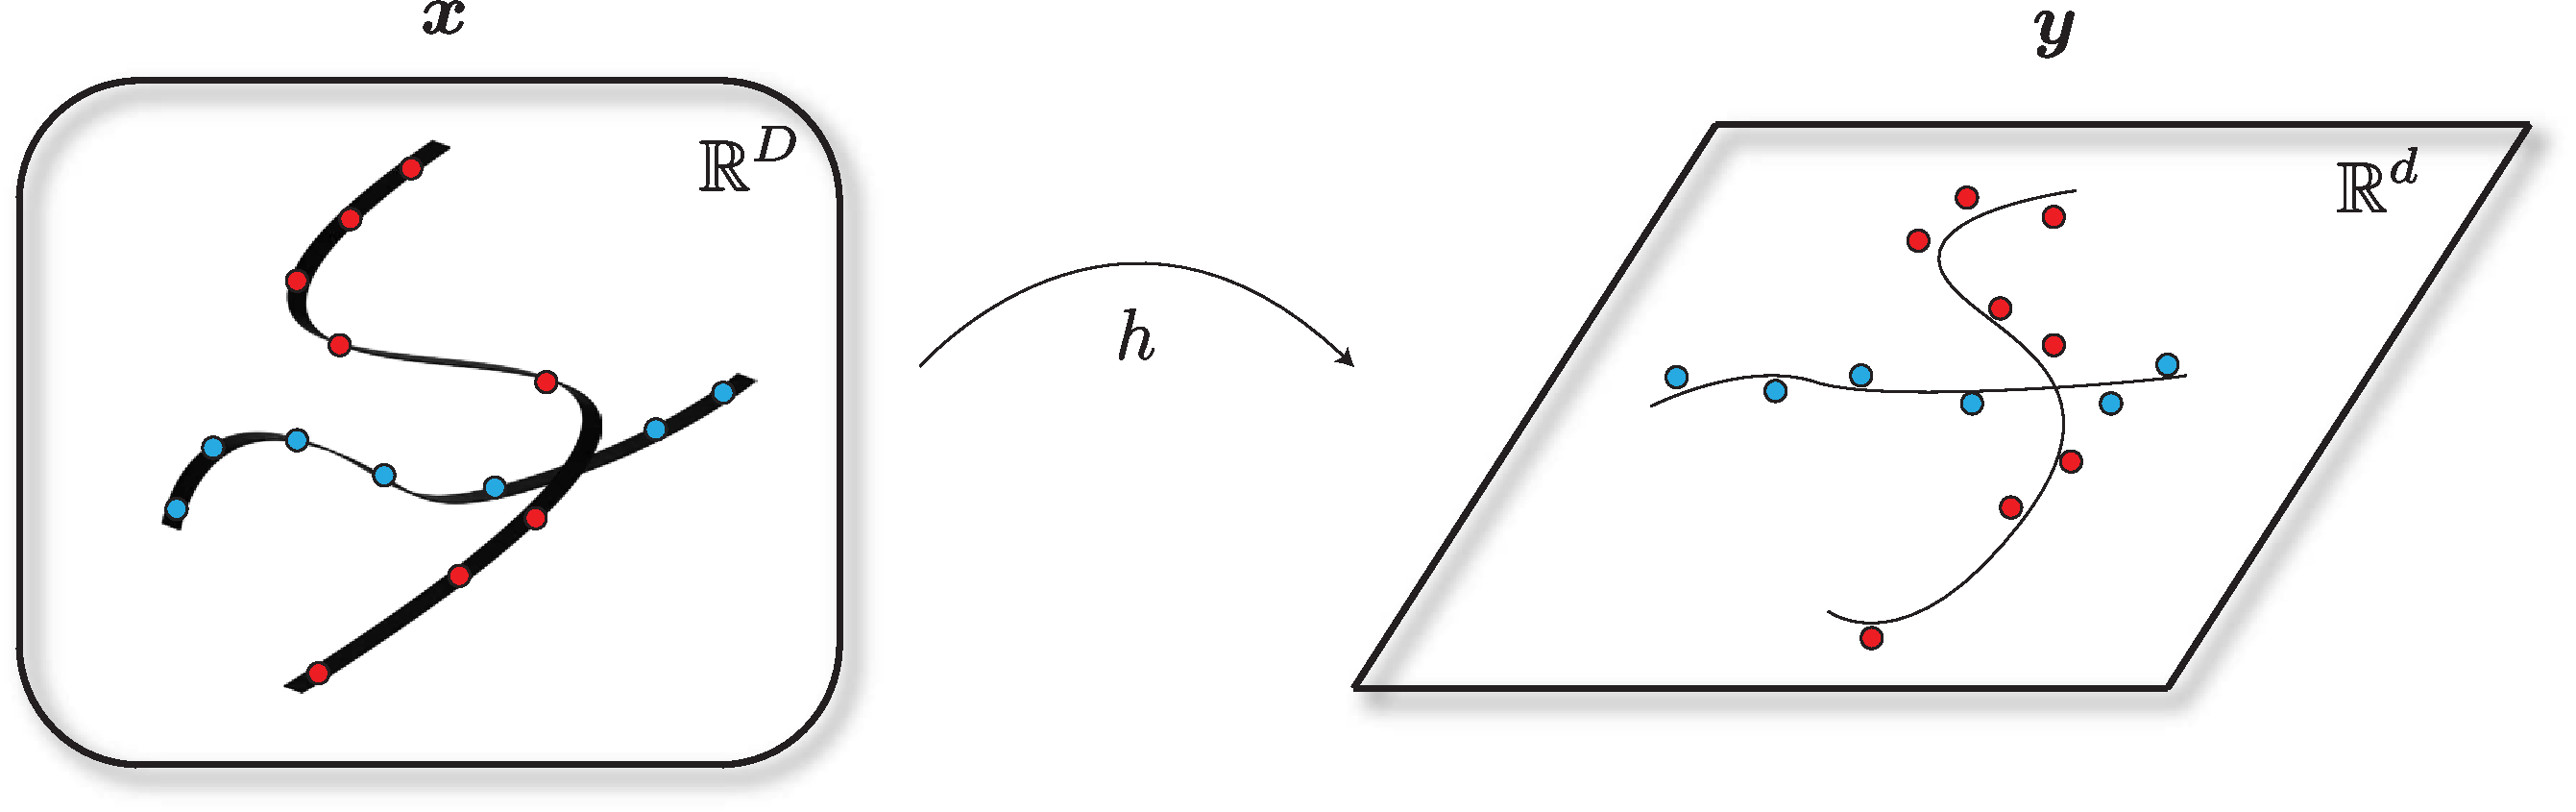
\includegraphics[width=0.9\textwidth]{\toplevelprefix/chapters/chapter6/figs/inference_roadmap.pdf}
  \caption{\small \textbf{Inference with low-dimensional distributions.} This is the generic picture for this chapter: we have a low-dimensional distribution for \(\vx \in \R^{D}\) (here depicted as a union of two \(2\)-dimensional manifolds in \(\R^{3}\)) and a measurement model \(\y = h(\vx) + \vw \in \R^{d}\). We want to infer various things about this model, including the conditional distribution of \(\vx\) given \(\vy\), or the conditional expectation \(\mathbb{E}[\vx \mid \y]\), given various information about the model and (potentially finite) samples of either \(\vx\) or \(\vy\).}
  \label{fig:inference_roadmap}
\end{figure}

\begin{example}[Image Completion and Text Prediction]
The popular natural image completion and natural language prediction are two typical tasks that require us to recover a full data $\x$ from its partial observations $\y$, with parts of $\x$ masked out and to be completed based on the rest. Figure \ref{fig:image-text-completion} shows some examples of such tasks. In fact, it is precisely these tasks which have inspired how to train modern large models for text generation (such as GPT) and image completion (such as the masked autoencoder) that we will study in greater details later.
    \begin{figure}
        \centering
        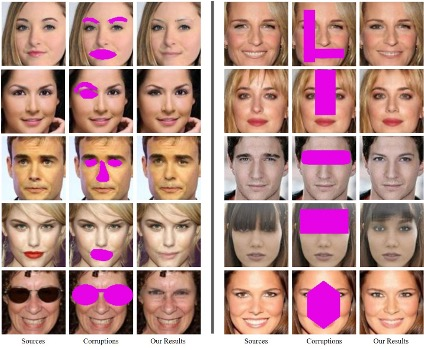
\includegraphics[height=0.4\linewidth]{\toplevelprefix/chapters/chapter6/figs/image-completion.jpg} \hspace{10mm} 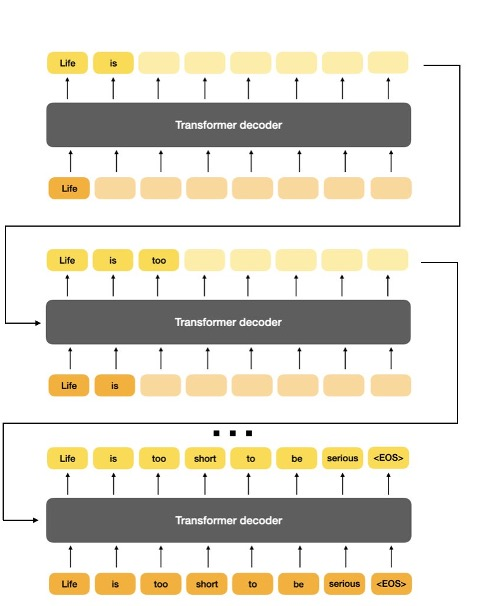
\includegraphics[height=0.45\linewidth]{\toplevelprefix/chapters/chapter6/figs/text-prediction.jpg}
        \caption{Left: image completion. Right: text prediction. In particular, text prediction is the inspiration for the popular Generative Pre-trained Transformer (GPT).}
        \label{fig:image-text-completion}
    \end{figure}
\end{example}


\paragraph{Statistical interpretation via Bayes' rule.} Generally speaking, to accomplish such tasks well, we need to get ahold of the conditional distribution $p(\x\mid \y)$. If we had this, then we would be able to find the maximal likelihood estimate (prediction): 
\begin{equation}
  \hat{\x} = \argmax_{\x} p(\x\mid \y);
\end{equation}
compute the conditional expectation estimate: 
\begin{equation}
  \hat{\x} = \mathbb{E}[\x \mid \y] = \int \x p(\x\mid \y)\odif{\vx};
\end{equation}
and sample from the conditional distribution:  
\begin{equation}
  \hat{\x} \sim p(\x \mid \y).
\end{equation}

Notice that from Bayes' rule, we have
\begin{equation}
  p(\x\mid \y) = \frac{p(\y\mid \x) p(\x) }{p(\y)}.
\end{equation} 
For instance, the maximal likelihood estimate can be computed by solving the following (maximal log likelihood) program:
\begin{equation}
    \hat{\x} = \argmax_{\x} [\log p(\y\mid \x) + \log p(\x)], 
\end{equation}
say via gradient ascent:
\begin{equation}
    \x_{k+1} = \x_k + \alpha \cdot \big(\nabla_{\x} \log p(\y \mid \x) + \nabla_{\x} \log p(\x)\big).
    \label{eqn:loglikelihoo-gradient-ascent}
\end{equation}
Efficiently computing the conditional distribution $p(\x \mid \y)$ naturally depends on how we learn and exploit the low-dimensional distribution $p(\x)$ of the data $\x$ and the observation model $\y = h(\x) + \vw$ that determines the conditional distribution $p(\y \mid \x)$. 

\begin{remark}[End-to-End versus Bayesian]
In the modern practice of data-driven machine learning, for certain popular tasks people often directly learn the conditional distribution $p(\x\mid \y)$ or a (probabilistic) mapping or a regressor. Such a mapping is often modeled by some deep networks and trained end-to-end with sufficient paired samples $(\x, \y)$. Such an approach is very different from the above Bayesian approach in which both the distribution of $\x \sim p(\x)$ and the (observation) mapping are needed. The benefit of the Bayesian approach is that the learned distribution $p(\x)$ can facilitate many different tasks with varied observation models and conditions. 
\end{remark}

\paragraph{Geometric interpretation as constrained optimization.}

As the support \(\cS_{\vx}\) of the distribution of \(\vx\) is low-dimensional, we may assume that there exists a function \(F\) such that
\begin{equation}
  F(\vx) = \boldsymbol{0} \qquad \iff \qquad \vx \in \cS_{\vx}
\end{equation}
such that \(\cS_{\vx} = F^{-1}(\{\vzero\})\) is the low-dimensional support of the distribution $p(\x)$. Geometrically, one natural choice of $F(\x)$ is the ``distance function'' to the support $\mathcal{S}_{\x}$:\footnote{Notice that, in reality, we only have discrete samples on the support of the distribution. In the same spirit of continuation, through diffusion or lossy coding studied in Chapter \ref{ch:compression}, we may approximate the distance function as $F(\x) \approx \min_{\x_p \in \cC_{\vx}^{\epsilon}} \|\x - \x_p\|_2$ where $\mathcal{S}_{\x}$ is replaced by a covering \(\cC_{\vx}^{\epsilon}\) of the samples with $\epsilon$-balls. }
\begin{equation}
    F(\x) = \min_{\x_p \in \mathcal{S}_{\x}} \|\x - \x_p\|_2. 
\end{equation}
Now given $\y = h(\x) +\vw$, to solve for $\x$, we can solve the following constrained optimization problem:
\begin{equation}
    \max_{\x} - \frac{1}{2}\|h(\x) - \y\|_2^2 \quad \mbox{s.t.} \quad F(\x) = \boldsymbol{0}. 
\end{equation}
Using the method of augmented Lagrange multipliers, we can solve the following unconstrained program:
\begin{equation}
   \max_{\x} \left[-\frac{1}{2}\|h(\x) - \y\|_2^2  + \vlambda^{\top} F(\x) - \frac{\mu}{2} \|F(\x)\|_2^2\right]
\end{equation}
for some constant Lagrange multipliers $\vlambda$.
This is equivalent to the following program:
\begin{equation}\label{eq:lagrange_multiplier_continuation}
\max_{\x} \left[\log \exp\Big(- \frac{1}{2}\|h(\x) - \y\|_2^2\Big) + \log \exp\Big( - \frac{\mu}{2} \big\|F(\x) - \vlambda/\mu\big\|_2^2\Big)\right],
\end{equation} 
where $\vc \doteq {\vlambda}/{\mu}$ can be viewed as a ``mean''  for the constraint function. As $\mu$ becomes large when enforcing the constraint via continuation\footnote{In the same spirit of continuation in \Cref{ch:compression} where we obtained better approximations of our distribution by sending \(\eps \to 0\), here we send \(\mu \to \infty\). Larger values of \(\mu\) will constrain \(F\) to take smaller and smaller values at the optimum, meaning that the optimum lies within a smaller and smaller neighborhood of the support \(\cS_{\vx}\). Interestingly, the theory of Lagrange multipliers hints that, under certain benign conditions on \(F\) and other terms in the objective, we only need to make \(\mu\) large enough in order to ensure \(F(\vx) = \vzero\) at the optimum, meaning that at \textit{finite} penalty we get \textit{perfect} approximation of the support. In general, we should have the intuition that \(\mu\) plays the same role as  \(\epsilon^{-1}\).}, $\|\vc\|_2$ becomes increasingly small.

The above program may be interpreted in two different ways. Firstly, one may view the first term as the conditional probability of $\y$ given $\x$, and the second term as a probability density for $\x$:
\begin{equation}
  p(\y\mid \x) \propto \exp\Big(- \frac{1}{2}\|h(\x) - \y\|_2^2\Big), \quad 
    p(\x) \propto \exp\Big( - \frac{\mu}{2}\|F(\x) - \vc\|_2^2\Big).
\end{equation} 
Hence, solving the constrained optimization for the inverse problem is equivalent to conducting Bayes inference with the above probability densities. Hence solving the above program \eqref{eq:lagrange_multiplier_continuation} via gradient ascent is equivalent to the above maximal likelihood estimate \eqref{eqn:loglikelihoo-gradient-ascent}, 
in which the gradient  takes the form:
\begin{equation}
   \nabla_{\x} \log p(\y \mid \x) + \nabla_{\x} \log p(\x)   =  \pdv{h}{\vx}(\vx)\big(\y - h(\x)\big) + \mu \pdv{F}{\vx}(\vx)\big(\vc - F(\x)\big),
\end{equation}
where $\pdv{h}{\vx}(\vx)$ and $\pdv{F}{\vx}(\vx)$ are the Jacobians of $h(\x)$ and $F(\x)$, respectively.

Secondly, notice that the above program \eqref{eq:lagrange_multiplier_continuation} is equivalent to:
\begin{equation}
\min_{\x} \frac{1}{2}\|h(\x) - \y\|_2^2 + \frac{\mu}{2} \big\|F(\x) - \vlambda/\mu\big\|_2^2,
\label{eqn:energy-minimization}
\end{equation} 
Due to the conspicuous quadratic form of the two terms, they can also be interpreted as certain ``energy'' functions. Such a formulation is often referred to as ``Energy Minimization'' in the machine learning literature.  



\paragraph{Several representative practical settings for inference.} 
In practice, however, initial information about the distributions of $\x$ and the relationship between $\x$ and $\y$ can be given in many different ways and forms. In general, they can mostly be categorized into four cases, which are, conceptually, increasingly more challenging:
\begin{itemize}
\item {\em Case 1:} Both a model for the distribution of $\x$ and the observation model $\y = h(\x)$ $(+ \boldsymbol{w})$ are known, even with an analytical form. This is typically the case for many classic signal processing problems, such as signal denoising, the sparse vector recovery problem we saw in Chapter \ref{ch:classic} and the low-rank matrix recovery problem to be introduced below.
\item {\em Case 2:} We do not have a model for the distribution but only samples $\X = \{\x_1, \ldots, \x_N\}$ of $\x$, and the observation model $\y = h(\x)$ $ (+ \boldsymbol{w})$ is known.\footnote{In the literature, this setting is sometimes referred to as the {\em empirical Bayesian inference}.} A model for the distribution $p(\x)$ of $\x$ needs to be learned, and subsequently the conditional distribution $p(\x\mid \y)$. Natural image completion or natural language completion (e.g., BERT and GPT) are typical examples of this class of problems.
\item {\em Case 3:} We only have the paired samples: $(\X, \Y) = \{ (\x_1, \y_1), \ldots, (\x_N, \y_N) \}$ of the two variables  $(\x, \y)$. The distributions of $\x$ and $\y$ and their relationship $h(\cdot)$ need to be learned from these paired sample data. For example, given many images and their captions, learning to conduct text-conditioned image generation is one such problem. 
\item {\em Case 4:} We only have the samples $\Y = \{\y_1, \ldots, \y_N\}$ of the observations $\y$, and the observation model $h(\cdot)$ needs to be known, at least in some parametric family $h(\cdot, \boldsymbol{\theta})$. The distribution $p(\x)$ and $p(\x \mid \y)$ need to be learned from $\hat \x$, estimated from $\Y$. For example, learning to render a new view from a sequence of calibrated or uncalibrated views is one such problem.
\end{itemize}
In this chapter, we will discuss general approaches to learn the desired distributions and solve the associated conditional estimation or generation for these cases, typically with a representative problem.  Throughout the chapter, you should keep \Cref{fig:inference_roadmap} in mind.





\section{Conditional Inference with a Known Data Distribution}
Notice that in the setting we have discussed in previous Chapters, the
autoencoding network is trained to reconstruct a set of samples of the random vector $\x$. This would allow us to regenerate samples from  the learned (low-dimensional) distribution. In practice, the low-dimensionality of the distribution, once given or learned, can be exploited for stable and robust recovery, completion, or prediction tasks. That is, under rather mild conditions, one can recover $\x$ from highly compressive, partial, noisy or even corrupted measures of $\x$ of the kind:
\begin{equation}
    \y = h(\x) + \vw,
\end{equation}
where $\y$ is typically an observation of $\x$ that is of much lower dimension than $\x$ and $\vw$ can be random noise or even sparse gross corruptions. This is a class of problems that have been extensively studied in the classical signal processing literature, for low-dimensional structures such as sparse vectors, low-rank matrices, and beyond. Interested readers may see \cite{Wright-Ma-2022} for a complete exposition of this topic.

Here to put the classic work in a more general modern setting, we illustrate the basic idea and facts through the arguably simplest task of data (and particularly image) completion. That is, we consider the problem of recovering a sample $\x$ when parts of it are missing (or even corrupted). We want to recover or predict the rest of $\x$
from observing only a fraction of it:
\begin{equation}
f: \mathcal{P}_{\Omega}(\x) \mapsto \hat{\x},
\end{equation}
where $\mathcal{P}_{\Omega}(\spcdot)$ represents a masking operation
(see \Cref{fig:matrix-completion} for an example).

In this section and the next, we will study the completion task under two different scenarios: One is when the distribution of the data $\x$ of interest is already given {\em apriori}, even in a certain analytical form. This is the case that prevails in classic signal processing where the structures of the signals are assumed to be known, for example,  band-limited, sparse or low-rank. The other is when only raw samples of $\x$ are available and we need to learn the low-dimensional distribution from the samples in order to solve the completion task well. This is the case for the tasks of natural image completion or video frame prediction. As a precursor to the rest of the chapter, we start with the simplest case of image completion: when the image to be completed can be well modeled as a low-rank matrix. We will move on to increasingly more general cases and more challenging settings later.

\paragraph{Low-rank matrix completion.}  
The low-rank {\em matrix
completion} problem is a classical problem for data completion when its distribution is low-dimensional and known. Consider a  random sample of a matrix $\X_o =
[\x_1, \ldots, \x_n] \in \mathbb{R}^{m\times n}$ from the space of all matrices of rank $r$. In general, we assume the rank
of the matrix is
\begin{equation}
\mbox{rank}(\X_o) = r < \min\{m, n\}.
\end{equation}
So it is clear that locally the intrinsic dimension of the space of all matrices of rank $r$ is much lower than the ambient space $mn$.

Now, let $\Omega$ indicate a set of indices of observed entries of the matrix $\X_o$. Let the observed entries be:
\begin{equation}
\Y = \mathcal{P}_{\Omega}(\X_o).
\end{equation}
The remaining entries supported on $\Omega^c$ are unobserved or
missing. The problem is whether we can recover from $\Y$ the missing
entries of $\X$ correctly and efficiently.  Figure \ref{fig:matrix-completion} shows one
example of completing such a matrix.

\begin{figure}
\centering
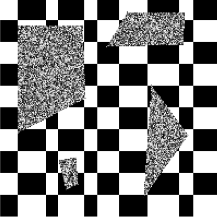
\includegraphics[width=0.3\linewidth]{\toplevelprefix/chapters/chapter6/figs/masked-checkerboard.png}\;\;
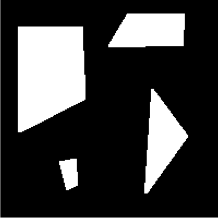
\includegraphics[width=0.3\linewidth]{\toplevelprefix/chapters/chapter6/figs/mask.png}\;\;
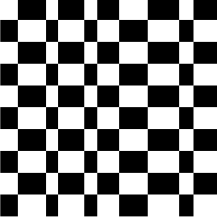
\includegraphics[width=0.3\linewidth]{\toplevelprefix/chapters/chapter6/figs/checkerboard.png}
\caption{Illustration of  completing an image as low-rank matrix
  with some entries masked or corrupted. Left: the masked/corrupted
image $\Y$; middle: the mask $\Omega$; right: the completed image $\hat \X$.}
\label{fig:matrix-completion}
\end{figure}

Notice that the fundamental reason why such a matrix can be completed is that columns and rows of the matrix are highly correlated and
they all lie on a low-dimensional subspace. For the example shown in
Figure \ref{fig:matrix-completion}, the dimension or the rank of the matrix completed is only two. Hence the fundamental idea to recover such a matrix is to seek a matrix that has the lowest rank among all
matrices that have entries agreeing with the observed ones:
\begin{equation}
\min_{\X} \mbox{rank}(\X) \quad \mbox{subject to}
\quad
\Y = \mathcal{P}_{\Omega}(\X).
\label{eqn:rank-min}
\end{equation}
This is known as the {\em low-rank matrix completion} problem. See \cite{Wright-Ma-2022} for a full characterization of the space of all low-rank matrices. As the rank function is discontinuous and rank minimization
is in general an NP-hard problem, we would like to relax it with
something easier to optimize.

Based on our knowledge about compression from Chapter
\ref{ch:compression}, we could  promote the low-rankness of the
recovered matrix $\X$ by enforcing the lossy coding rate (or the
volume spanned by $\X$) of the data in $\X$ to be small:
\begin{equation}
\min R_\epsilon(\X) = \frac{1}{2} \log \det \left(\boldsymbol{I} +
\alpha  \X\X^\top \right) \quad \mbox{subject to}
\quad
\Y = \mathcal{P}_{\Omega}(\X).
\label{eqn:rate-min}
\end{equation}
The problem can viewed as a continuous relaxation of the above
low-rank matrix completion problem \eqref{eqn:rank-min} and it can be
solved via gradient descent. One can show that the gradient descent
operator for the $\log\det$ objective is precisely minimizing a close
surrogate of the rank of the matrix $\X\X^\top$.

The rate distortion function is a nonconvex function, and its gradient
descent does not always guarantee finding the globally optimal solution. Nevertheless, since the underlying structure sought for $\X$ is piecewise linear, the rank function admits a rather effective convex relaxation: the
nuclear norm---the sum of all singular values of the matrix $\X$. As
shown in the compressive sensing literature, under fairly
broad conditions,\footnote{Typically, such conditions specify the
necessary and sufficient amount of entries needed for the completion
to be computationally feasible. These conditions have been
systematically characterized in \cite{Wright-Ma-2022}.} the matrix
completion problem \eqref{eqn:rank-min}
can be effectively solved by the following convex program:
\begin{equation}
\min \|\X\|_* \quad \mbox{subject to}
\quad
\Y = \mathcal{P}_{\Omega}(\X),
\label{eqn:nuclear-min}
\end{equation}
where the nuclear norm $\|\X\|_*$ is the sum of singular values of
$\X$. In practice, we often convert the above constrained convex optimization
program to an unconstrained one:
\begin{equation}
\min \|\X\|_*  + \lambda \|
\Y - \mathcal{P}_{\Omega}(\X)\|_F^2,
\label{eqn:nuclear-min-lagrangian}
\end{equation}
for some properly chosen $\lambda > 0$. Interested readers may refer to
\cite{Wright-Ma-2022} for how to develop algorithms  that can solve
the above programs  efficiently and effectively.
Figure \ref{fig:matrix-completion} shows a real example in which the
matrix $\hat \X$ is actually recovered by solving the above program.

\paragraph{Further extensions.}
It has been shown that images (or more accurately textures) and 3D scenes
with low-rank structures can be very effectively completed via
solving optimization programs of the above kind, even if there is
additional corruption and distortion
\cite{Zhang2010TILTTI,Liang-ECCV2012,Yi_2023_ICCV}:
\begin{equation}
    \Y \circ \tau = \X_o + \boldsymbol{E},
\end{equation}
where $\tau$ is some unknown nonlinear distortion of the image and $\boldsymbol{E}$ is an unknown matrix that models some (sparse) occlusion and corruption. Again, interested readers may refer to \cite{Wright-Ma-2022} for a more detailed account.

\section{Conditional Inference with a Learned Data Representation}
In the previous subsection, the reason we can infer $\x$ from the partial observation $\y$ is because (support of) the distribution of $\X$ is known or specified {\em apriori}, say as the set of all low-rank matrices. For many practical datasets, we do not have their distribution in an analytical form like the low-rank matrices, say the set of all natural images. Nevertheless, if we have sufficient samples of the data $\x$, we should be able to learn its low-dimensional distribution first and leverage it for future inference tasks based on an observation $\y = h(\x) + \vw$. In this section, we assume the observation model $h(\cdot)$ is given and known. We will study the case when $h(\cdot)$ is not explicitly given in the next section.


\subsection{Image Completion with Masked Auto-Encoding}
For a general image $\vX$ such as the one shown on the left of Figure
\ref{fig:crate_mae_pipeline}, we can no longer view it as a low-rank
matrix. However, humans still demonstrate remarkable ability to
complete a scene and recognize familiar objects despite severe
occlusion. This suggests that our brain has learned the
low-dimensional distribution of natural images and can use it for
completion, and hence recognition. However, the distribution of all
natural images is not as simple as a low-dimensional linear subspace.
Hence a natural question is whether we can learn the more
sophisticated distribution of natural images and use it to perform
image completion?

\begin{figure}[t!]
\begin{center}
  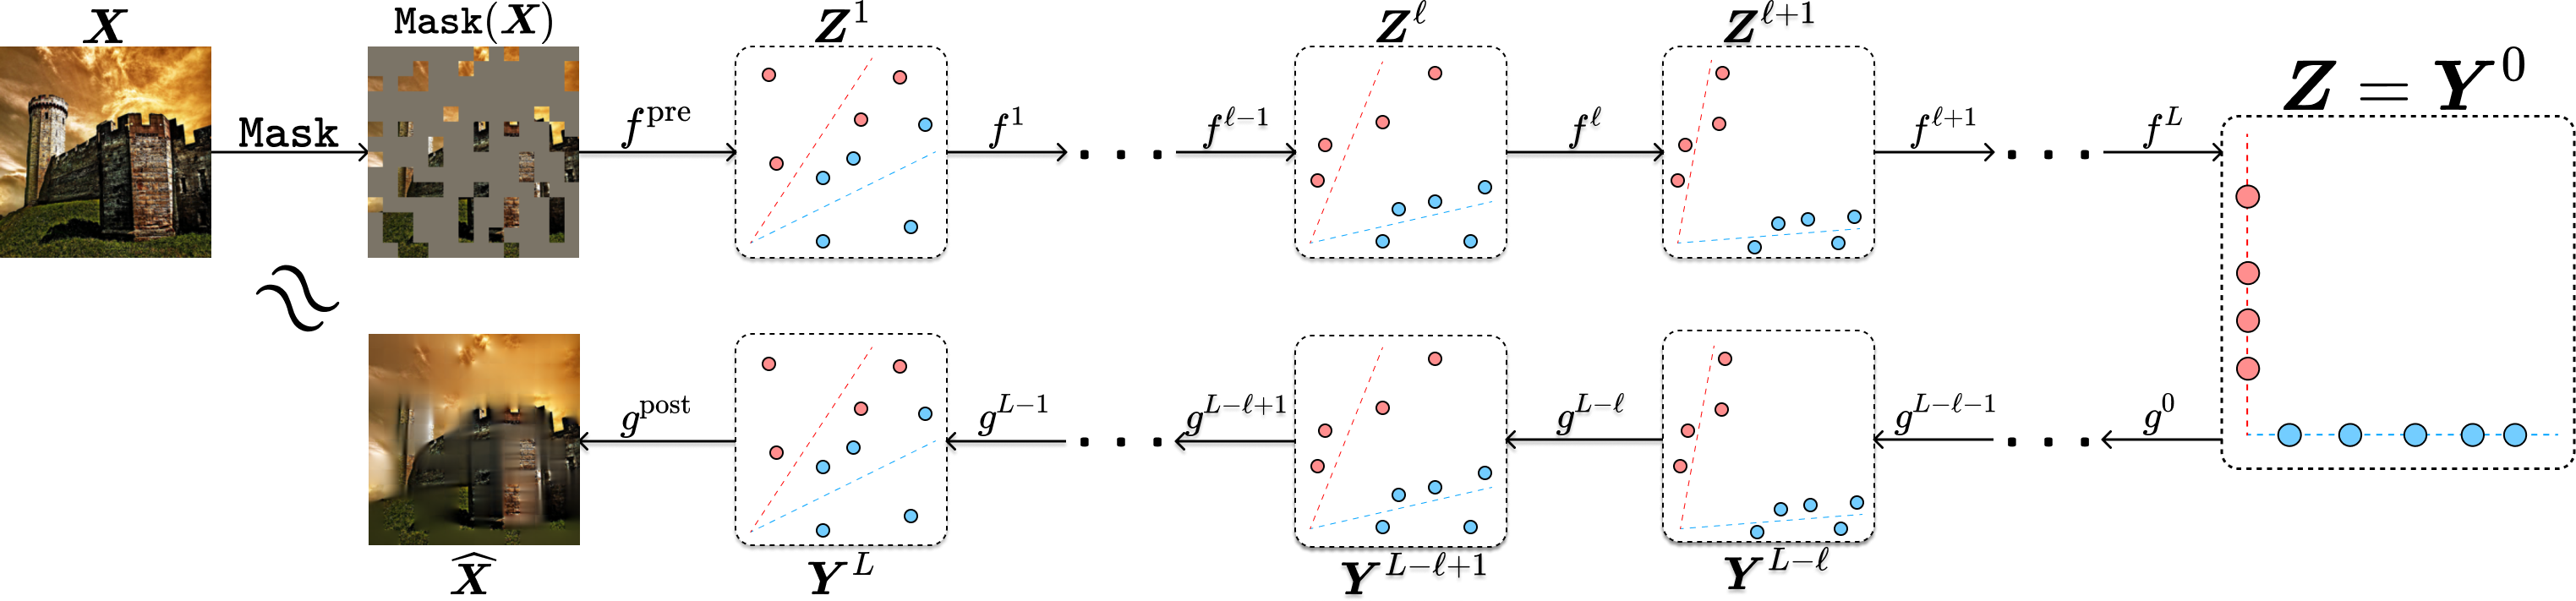
\includegraphics[width=0.99\textwidth]{\toplevelprefix/chapters/chapter6/figs/crate_mae_pipeline.png}
\end{center}
\caption{\small \textbf{Diagram of the overall  (masked)
  autoencoding process.} The (image) token representations are
  transformed iteratively towards a parsimonious (e.g., compressed
  and sparse) representation by each encoder layer \(f^{\ell}\).
  Furthermore, such representations are transformed back to the
  original image by the decoder layers \(g^{\ell}\). Each encoder
  layer \(f^{\ell}\) is meant to be (partially) inverted by a
corresponding decoder layer \(g^{L - \ell}\).}
\label{fig:crate_mae_pipeline}
\end{figure}

One empirical approach to the image completion task is to find an encoding and decoding scheme by
solving the following {\em masked autoencoding} (MAE) program that
minimizes the reconstruction loss:
\begin{equation}\label{eq:mae_loss}
\min_{f, g} L_{\mathrm{MAE}}(f, g) \doteq \mathbb{E}\big[\norm{(g \circ
f)(\mathcal{P}_\Omega(\vX)) - \vX}_{2}^{2}].
\end{equation}
Unlike the matrix completion problem which has a simple underlying
structure, we should no longer expect that the encoding and decoding
mappings admit simple closed forms or the program can be solved by
explicit algorithms.

For a general natural image, we can no longer assume that its columns or
rows are sampled from a low-dimensional subspace or a low-rank
Gaussian. However, it is reasonable to assume that the image consists
of multiple regions. Image patches in each region are similar and can
be modeled as one (low-rank) Gaussian or subspace. Hence, to exploit
the low-dimensionality of the distribution, the objective \textit{of the
encoder} $f$ is to transform $\X$ to a representation $\Z$:
\begin{equation}
    f: \X \mapsto \Z
\end{equation}
such that the distribution of $\Z$ can be well modeled as a mixture of subspaces, say $\{\vU_{[K]}\}$,
such that the rate reduction is maximized while the sparsity is minimized:
\begin{equation}\label{eq:sparse_rr}
\mathbb{E}_{\vZ = f(\vX)}[\Delta R_{\epsilon}(\vZ \mid \vU_{[K]}) - \lambda
\norm{\vZ}_{0}] = \mathbb{E}_{\vZ = f(\vX)}[R_\epsilon(\vZ) - R^{c}_\epsilon(\vZ \mid
\vU_{[K]}) - \lambda \norm{\vZ}_{0}],
\end{equation}
where the functions $R_\epsilon(\cdot)$ and $R^c_\epsilon(\cdot)$ are defined in \eqref{eq:coding_rate} and \eqref{eq:def-mcr-Rc}, respectively. 

As we have shown in the previous Chapter \ref{ch:representation}, the
encoder $f$ that minimizes the above objective can be constructed as
a sequence of transformer-like operators. As shown in the work of
\cite{Pai2024masked}, the decoder $g$ can be viewed and hence
constructed explicitly as the inverse process of the encoder $f$.
Figure \ref{fig:crate_mae_layers} illustrates the overall
architectures of both the encoder and the corresponding decoder at
each layer. The parameters of the encoder $f$ and decoder $g$ can be
learned by optimizing the reconstruction loss \eqref{eq:mae_loss} via
gradient descent.

\begin{figure}[t!]
\centering
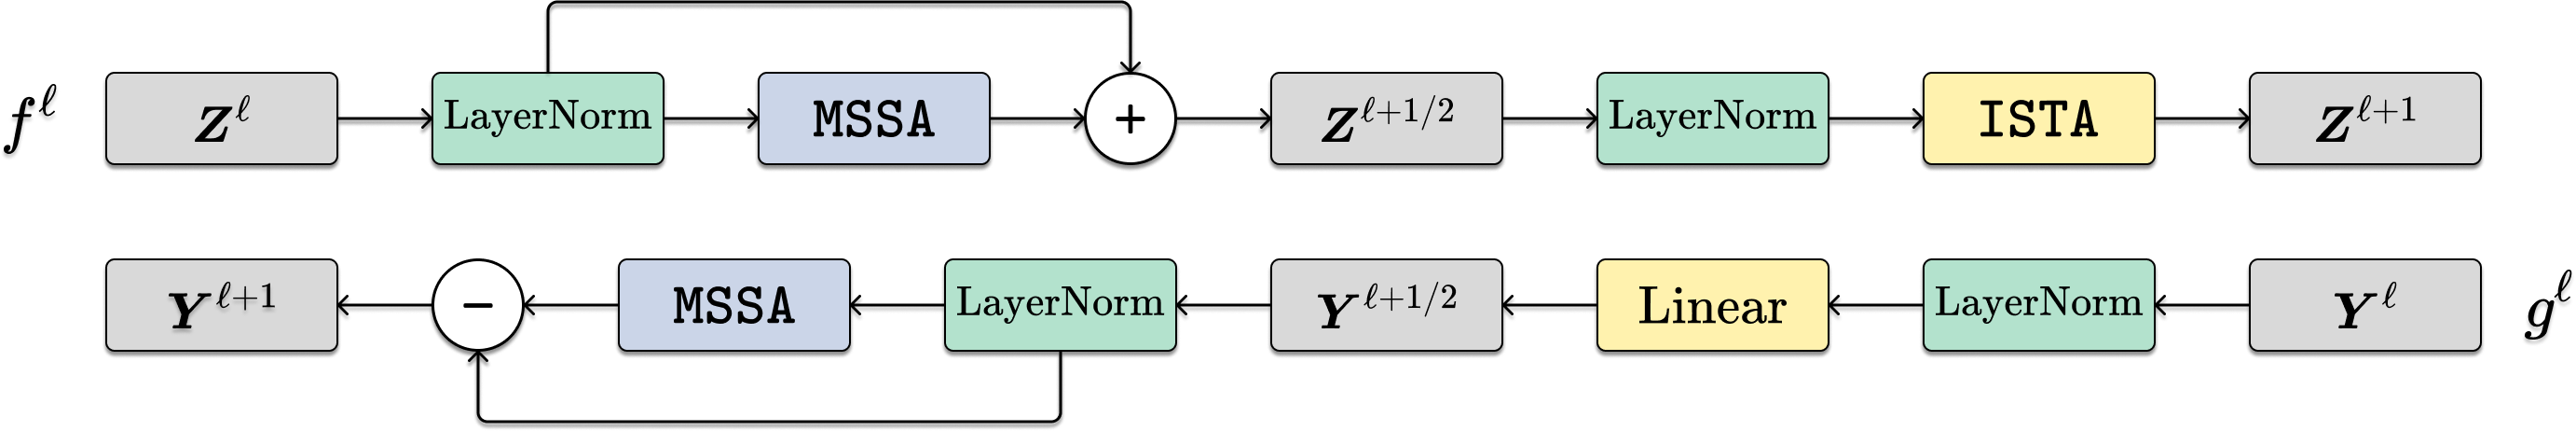
\includegraphics[width=0.99\textwidth]{\toplevelprefix/chapters/chapter6/figs/crate_mae_layers.png}
\caption{\small \textbf{Diagram of each encoder layer
  (\textit{top}) and decoder layer (\textit{bottom}).} Notice that
  the two layers are highly anti-parallel --- each is constructed to
  do the operations of the other in reverse order. That is, in the
  decoder layer \(g^{\ell}\), the \(\ISTA\) block of \(f^{L - \ell}\)
  is partially inverted first using a linear layer, then the
  \(\MSSA\) block of \(f^{L - \ell}\) is reversed; this order
unravels the transformation done in \(f^{L - \ell}\).}
\label{fig:crate_mae_layers}
\end{figure}

Figure \ref{fig:mae_autoencoding-small} shows some representative
results of the thus-designed masked auto-encoder. More implementation details and
results of the masked autoencoder for natural image completion can be
found in Chapter \ref{ch:applications}.
\begin{figure}[t]
\centering
\includegraphics[width=0.99\textwidth]{\toplevelprefix/chapters/chapter6/figs/crate_mae_autoencoding_small.pdf}
\caption{\small \textbf{Autoencoding visualizations of CRATE-Base
  and ViT-MAE-Base \cite{he2022masked} with 75\% patches masked.}
  We observe that the reconstructions from CRATE-Base are on par
  with the reconstructions from ViT-MAE-Base, despite using \(<
  1/3\) of the parameters.
}
\label{fig:mae_autoencoding-small}
\end{figure}





\subsection{Conditional Sampling with Measurement Matching}
\label{sec:conditioned-decoding}
The above (masked) autoencoding problem aims to generate a sample image that is consistent with certain observations or conditions. But let us examine the approach more closely: given the
visual part of an image $\X_v = \mathcal{P}_{\Omega}(\X)$, we try to
estimate the masked part $\X_m = \mathcal{P}_{\Omega^c}(\X)$. For realizations
$(\vXi_v, \vXi_m)$ of the random variable $\vX=(\vX_v, \vX_m)$, let
\[p_{\X_m \mid \X_v}(\vXi_m\mid \vXi_v)\]
be the conditional distribution of $\X_m$ given
$\X_v$. It is easy to show that the optimal solution to the  MAE
formulation \eqref{eq:mae_loss} is given by the conditional expectation:
\begin{equation}
  \argmin_{h = g \circ f}\, L_{\mathrm{MAE}}(h)
  = \vXi_v \mapsto \vXi_v + \mathbb{E}[\X_m \mid \X_v=\vXi_v].
\end{equation}
In general, however, this expectation may not even lie on the
low-dimensional distribution of natural images! This partially
explains why some of the recovered patches in \Cref{fig:mae_autoencoding-small}
are a little blurry.

For many practical purposes, we would like to learn (a representation
of) the conditional distribution $p_{\X_m \mid \X_v}$, or equivalently
$p_{\X \mid \X_v}$,
and then get a clear (most likely) sample from this distribution directly. Notice that, when the distribution of $\X$ is low-dimensional, it is possible that if a
sufficient part of $\X$, $\X_v$, is observed, it fully determines
$\X$ and hence the missing part $\X_m$. In other words, the distribution
$p_{\X \mid \X_v}$ is a generalized function---if $\vX$ is fully determined by $\vX_v$ it is the delta function, and more generally one of its exotic cousins.

Hence, instead of solving the completion task as a conditional estimation problem, we should address it as a conditional sampling problem. To that end, we should first learn the (low-dimensional) distribution of all natural images $\X$. If we have sufficient samples of natural images, we can learn the distribution via a denoising process $\X_t$ described in Chapter \ref{ch:compression}. Then the problem of recovering $\X$ from its partial observation $\Y = \mathcal{P}_\Omega(\x) +\vw$ becomes a conditional generation problem -- to sample the distribution conditioned on the observation.

\begin{figure}
  \centering
  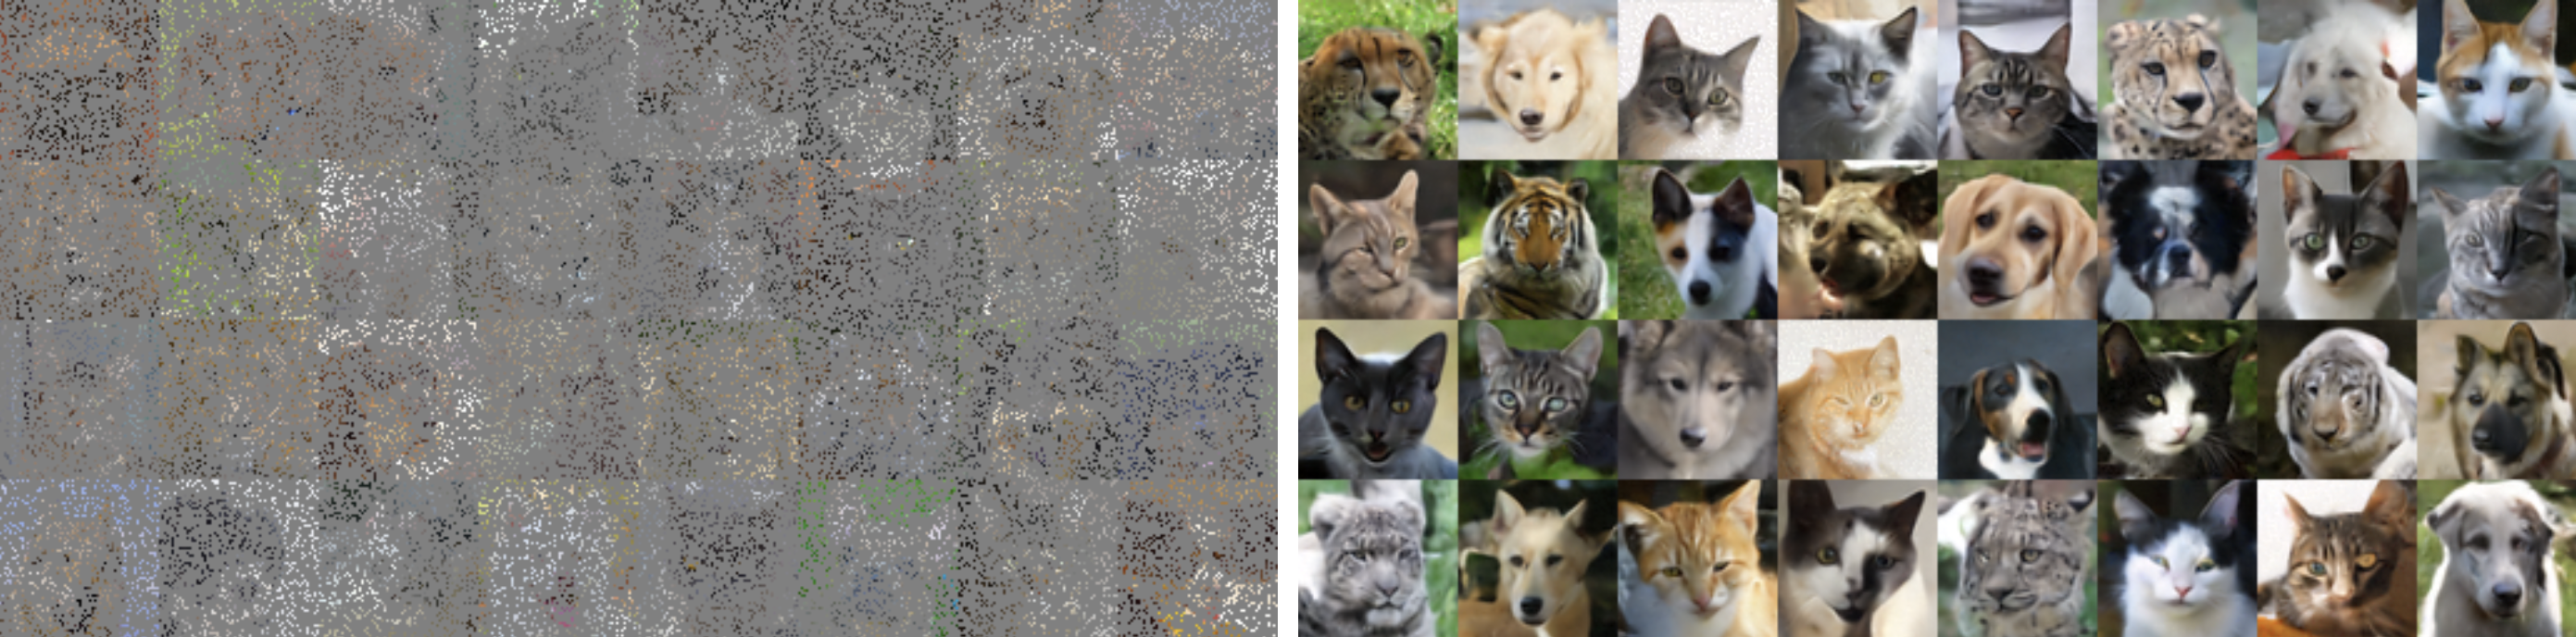
\includegraphics[width=1.0\textwidth]{\toplevelprefix/chapters/chapter6/figs/ambient_diffusion.png}
  \caption{\small \textbf{Sampling visualizations from models trained via ambient diffusion \cite{Daras-NIPS2023} with 80\% of the pixels masked.} Using a similar ratio of masked pixels as in \Cref{fig:mae_autoencoding-small}, the ambient diffusion sampling algorithm recovers a much sharper image than the blurry image recovered by the MAE-based method. The former method samples from the distribution of natural images, while the latter approximates the conditional expectation (i.e., average) of this distribution given the observation; this averaging causes the blurriness.}
  \label{fig:ambient_diffusion}
\end{figure}

\paragraph{General linear measurements.} 
In fact, we may even consider recovering $\X$ from a more general linear observation model:
\begin{equation}
    \Y = \vA\X_0,  \quad \X_t = \X_0 + \sigma_t \vG,  
\end{equation}
where $\vA$ is a linear operator on matrix space\footnote{i.e., if we imagine unrolling \(\vX\) into a long vector then \(\vA\) takes the role of a matrix on \(\vX\)-space} and $\vG \sim \mathcal{N}(\boldsymbol{0}, \vI)$. The masking operator $\mathcal{P}_{\Omega}(\cdot)$ in the image completion task is one example of such a linear model. Then it has been shown by \cite{daras2023ambient} that 
\begin{equation}
    \hat{\X}_* = \argmin_{\hat{\X}} \mathbb{E}[\|\vA(\hat{\X}(\vA\X_t, \vA) - \X_0)\|^2]
\end{equation}
satisfies the condition that:
\begin{equation}
    \vA \hat{\X}_*(\vA(\X_t), \vA) = \vA \mathbb{E}[\X_0 \mid \vA \X_t, \vA].
\end{equation} Notice that in the special case when $\vA$ is of full column rank, we have $ \mathbb{E}[\X_0 \mid \vA\X_t, \vA] = \mathbb{E}[\X_0 \mid \X_t]$. Hence, in the more general case, it has been suggested by \cite{daras2023ambient} that one could still use the so obtained $\mathbb{E}[\X_0 \mid \vA(\X_t), \vA]$ to replace the $\mathbb{E}[\X_0 \mid \X_t]$ in the normal denoising process for $\X_t$:
\begin{equation}
    \X_{t-s} = \gamma_t \X_t + (1-\gamma_t) \mathbb{E}[\X_0 \mid \vA\X_t, \vA].
\end{equation}
This usually works very well in practice, say for many image restoration tasks, as shown in \cite{daras2023ambient}. Compared to the blurry images recovered from MAE, the images recovered by the above method are much sharper as it leverages a learned distribution of natural images and samples a (sharp) image from the distribution that is consistent with the measurement, as shown in \Cref{fig:ambient_diffusion} (cf \Cref{fig:mae_autoencoding-small}).


\paragraph{General nonlinear measurements.}
To generalize the above (image) completion problems and make things more rigorous, we may consider that a random vector $\vx \sim p$ is partially observed through a more
general observation function:
\begin{equation}\label{eq:measurement-matching-observation}
\vy = h(\vx) + \vw,
\end{equation}
where $\vw$ usually stands for some random measurement noise, say of
a Gaussian distribution $\vw \sim \mathcal{N}(\mathbf{0}, \sigma^2
\boldsymbol{I})$. It is easy to see that, for $\x$ and $\y$ so related, their joint distribution $p(\x, \y)$ is naturally nearly degenerate if the noise $\vw$ is small. To a large extent, we may view $p(\x, \y)$ as a noisy version of a hypersurface defined by the function $\y = h(\x)$ in the joint space $(\x, \y)$.  Practically speaking, we will consider a setting more akin to masked autoencoding than to pure matrix completion, where we always have access to a corresponding clean sample $\vx$ for every observation $\vy$ we receive.\footnote{In some more specialized applications, in particular in scientific imaging, it is of interest to be able to learn to generate samples from the posterior $p_{\x \mid \y}$ without access to any clean/ground-truth samples of $\x$. We give a brief overview of methods for this setting in the end-of-chapter notes.}

Like image/matrix completion, we
are often faced with a setting where $\vy$ denotes a degraded or otherwise
``lossy''
observation of the input $\vx$. This can manifest in quite different
forms. For example, in various scientific or
medical imaging problems, the measured data $\vy$ may be a compressed and
corrupted observation of the underlying data $\vx$; whereas in 3D vision tasks,
$\vy$ may represent an image captured by a camera of a physical object with an
unknown (low-dimensional) pose $\vx$.
Generally, by virtue of mathematical modeling (and, in some cases, co-design
of the measurement system), we know $h$ and can evaluate it on any input, and
we can exploit this knowledge to help reconstruct and sample $\vx$.

\begin{figure}[t]
  \centering
  \begin{subfigure}{0.45\textwidth}
    \vspace{0.75cm}
    \centering
    \begin{tikzcd}[column sep=1.5cm]
      \vx \arrow[r, "h(\vx) + \vw"] & \vy \arrow[r, "p_{\vx \mid \vy}"]
      & \posteriorsample \arrow[r, "\posteriorsample + t\vg"] & \posteriorsample_t
    \end{tikzcd}
    \vspace{0.75cm}
    \caption{}
    \label{fig:left}
  \end{subfigure}
  \hfill
  \begin{subfigure}{0.45\textwidth}
    \centering
    \begin{tikzcd}[column sep=1.5cm, row sep=0.5cm]
    & \vy \\
    \vx \arrow[ur, "h(\vx) + \vw"] \arrow[dr, "\vx + t\vg"] & \\
    & \vx_t
    \end{tikzcd}
    \caption{}
    \label{fig:right}
  \end{subfigure}
  \caption{Statistical dependency diagrams for the conditional sampling process.
  \textbf{Left:} In a direct (conceptual) application of the diffusion-denoising scheme
  we have developed in \Cref{ch:compression} to conditional sampling, we use
  samples from the posterior $p_{\vx \mid \vy}$ to train denoisers directly on
  the posterior at different noise levels, then use them to generate new
  samples. In practice, however, we do not normally have direct samples from the
  posterior, but rather paired samples $(\vx, \vy)$ from the joint.
  \textbf{Right:} It turns out that it suffices to have only noisy observations
  of $\vx$ to realize the denoisers corresponding to $p_{\posteriorsample_t \mid
  \posteriorsample}$: this follows from conditional independence of $\vx_t$ and
  $\vy$ given $\vx$. It implies that $p_{\posteriorsample_t} = p_{\vx_t \mid
  \vy}$, which gives a score function for denoising that consists of the
  unconditional score function, plus a correction term that enforces measurement
  consistency.}
  \label{fig:posterior-sampling-cds}
\end{figure}


At a technical level, we want the learned representation of the data
to facilitate us to sample the conditional distribution $p_{\vx\mid
\vy}$, also known as the posterior, effectively and efficiently. More precisely,
write $\vnu$ to denote a realization of the random variable $\vy$.
We want to generate samples $\hat{\x}$ such that:
\begin{equation}\label{eq:goal-sample-posterior}
  \hat{\x} \sim   p_{\vx \mid \y}(\spcdot \mid \vy=\vnu).
\end{equation}

Recall that in \Cref{sub:compression_denoising}, we have developed a natural and
effective way to produce \textit{unconditional} samples of the data distribution
$p$. The ingredients are the denoisers $\bar{\x}^\ast(t, \vxi) = \bE[ \x \mid
\vx_t=\vxi ]$, or their learned approximations $\bar{\x}_{\theta}(t, \vxi)$,
for different levels of noisy observations $\x_t = \x + t \vg$ (and $\vxi$ for
their realizations) under
Gaussian noise $\vg \sim \cN(\mathbf{0}, \vI)$, and $t \in
[0, T]$ with a choice of times $0 = t_1 < \hdots < t_{L} = T$ at which to
perform the iterative denoising, starting from $\hat{\vx}_{t_L} \sim
\cN(\mathbf{0}, T^2 \vI)$ (recall \Cref{eq:denoising-iteration-basic}).\footnote{Recall from our discussion in \Cref{sub:sampling_denoising}
that a few small improvements to this basic iterative denoising scheme are
sufficient to bring competitive practical performance. For clarity as we develop
conditional sampling, we will focus here on the simplest instantiation.}
We could directly apply this scheme to generate samples from the posterior
$p_{\vx \mid \vy}$ \textit{if} we had access to a dataset of samples
$\posteriorsample \sim p_{\vx \mid \y}(\spcdot \mid \vnu)$ for each realization
$\vnu$ of $\vy$, by generating noisy observations
$\posteriorsample_t$ and training denoisers to approximate $\bE[
  \posteriorsample \mid \posteriorsample_t=\spcdot, \vy=\vnu ]$, the mean of the posterior under
the noisy observation (see \Cref{fig:posterior-sampling-cds}(a)).
However, performing this resampling given only paired samples $(\vx, \vy)$ from the
joint distribution (say by binning the samples over values of $\vy$) requires
prohibitively many samples for high-dimensional data, and alternate approaches
explicitly or implicitly rely on density estimation, which similarly suffers from the
curse of dimensionality.

Fortunately, it turns out that this is not necessary.
Consider the alternate statistical dependency diagram in
\Cref{fig:posterior-sampling-cds}(b), which corresponds to the random variables
in the usual denoising-diffusion process, together with the measurement $\vy$. 
Because our assumed observation model \eqref{eq:measurement-matching-observation}
implies that $\vx_t$ and $\vy$ are independent conditioned on $\vx$, we have for
any realization $\vnu$ of $\vy$
\begin{equation}\label{eq:conditional-denoising-conditioning-order-irrelevant}
  \begin{split}
  p_{\posteriorsample_t\mid \vy}(\spcdot \mid \vnu)
  &= \int
  \underbrace{p_{\posteriorsample_t \mid \posteriorsample}(\spcdot\mid \vxi)}_{=
  \cN(\vxi, t^2 \vI)}
  \spcdot \underbrace{p_{\posteriorsample \mid \vy}}_{= p_{\vx\mid \vy}}(\vxi \mid
  \vnu)
  \odif \vxi
  \\
  &=
  \int p_{\vx_t \mid \vx, \vy}(\spcdot\mid \vxi, \vnu) \spcdot p_{\vx \mid
  \vy}(\vxi\mid \vnu) \odif \vxi
  \\
  &=
  \int p_{\vx_t, \vx \mid \vy}(\spcdot, \vxi \mid \vnu) \odif \vxi
  \\
  &= p_{\vx_t \mid \vy}(\spcdot\mid \vnu).
  \end{split}
\end{equation}
Above, the first line recognizes an equivalence between the distributions
arising in \Cref{fig:posterior-sampling-cds} (a,b); the second line applies this
together with conditional independence of $\vx_t$ and $\vy$ given $\vx$; the
third line uses the definition of conditional probability; and the final line
marginalizes over $\vx$.
Thus, the denoisers from the conceptual posterior sampling process are equal to
$\bE[\vx \mid \vx_t=\spcdot, \vy=\vnu]$, which we can learn solely from paired samples $(\vx,
\vy)$,
and by Tweedie's formula (\Cref{thm:tweedie}), we can express these denoisers in
terms of the score function of $p_{\vx_t \mid \vy}$, which, by Bayes' rule,
satisfies
\begin{equation}
  p_{\vx_t \mid \vy}(\vxi \mid \vnu) 
  = \frac{p_{\vy \mid \vx_t}(\vnu \mid \vxi) p_{\vx_t}(\vxi)}{p_{\vy}(\vnu)}.
\end{equation}
Recall that the density of $\vx_t$ is 
given by $p_t = \varphi_{t} \ast p$, where $\varphi_{t}$ denotes the standard
Gaussian density with zero mean and covariance $t^2 \vI$ and $\ast$ denotes
convolution. This is nothing but the \textit{unconditional score function}
obtained from the standard diffusion training that we developed in
\Cref{sub:compression_denoising}!
The conditional score function then satisfies, for any realization $(\vxi,
\vnu)$ of $(\vx_t, \vy)$,
\begin{equation}
  \nabla_{\vxi} \log p_{\vx_t \mid \vy}(\vxi\mid \vnu)
  =
  \underbrace{\nabla_{\vxi} \log p_t(\vxi)}_{\text{score matching}}
  +
  \underbrace{\nabla_{\vxi} \log p_{\vy \mid \vx_t}(\vnu \mid \vxi)}_{\text{measurement matching}},
  \label{eqn:conditional-denoising-score}
\end{equation}
giving (by Tweedie's formula) our proposed denoisers as
\begin{align*}
  \bE[ \vx \mid \vx_t=\vxi, \vy=\vnu]
  &=
  \vxi + t^2 \nabla_{\vxi}\log p_t(\vxi) + t^2 \nabla_{\vxi}\log p_{\vy \mid
  \vx_t}(\vnu \mid \vxi)
  \\
  &=
  \bE[\vx \mid \vx_t=\vxi] + t^2 \nabla_{\vxi}\log p_{\vy \mid \vx_t}(\vnu\mid
  \vxi).
  \labelthis \label{eq:posterior-sampling-denoiser-decomposition}
\end{align*}
The resulting operators are interpretable as a \textit{corrected} version of the
unconditional denoiser for the noisy observation, where the correction term (the
so-called ``measurement matching'' term) enforces consistency with the
observations $\vy$. The reader should take care to note to which argument the
gradient operators are applying in the above score functions in order to fully
grasp the meaning of this operator.

The key remaining issue in making this procedure computational is to prescribe
how to compute the measurement matching correction, since in general we do not
have a closed-form
expression for the likelihood $p_{\vy \mid \vx_t}$ except for when $t
= 0$. Before taking up this problem, we discuss an illustrative concrete example
of the entire process, continuing from those we have developed in
\Cref{sub:compression_denoising}.

\begin{example}\label{example:denoising-conditional-gaussian}
  Consider the case where the data distribution is Gaussian with mean $\vmu \in
  \bR^D$ and
  covariance $\vSigma \in \bR^{D \times D}$, i.e., $\vx \sim \cN(\vmu, \vSigma)$.
  Assume that $\vSigma \succeq \Zero$ is nonzero.
  Moreover, in the measurement model \eqref{eq:measurement-matching-observation},
  suppose we obtain linear measurements of $\vx$ with independent Gaussian
  noise, where $\vA \in \bR^{d \times D}$ and $\vy = \vA \vx + \sigma \vw$
  with $\vw \sim \cN(\Zero, \vI)$ independent of $\vx$.
  Then $\vx =_{d} \vSigma^{1/2} \vg + \vmu$, where $\vg \sim \cN(\Zero, \vI)$ is
  independent of $\vw$ and $\vSigma^{1/2}$ is the unique positive square root of
  the covariance matrix $\vSigma$, and
  after some algebra, we can then write
  \begin{equation*}
    \begin{bmatrix}
      \vx \\
      \vy
    \end{bmatrix}
    =_{d}
    \begin{bmatrix}
      \vSigma^{1/2} & \Zero \\
      \vA \vSigma^{1/2} & \sigma \vI
    \end{bmatrix}
    \begin{bmatrix}
      \vg \\
      \vw
    \end{bmatrix}
    +
    \begin{bmatrix}
      \vmu \\
      \vA\vmu
    \end{bmatrix}.
  \end{equation*}
  By independence, we have that $(\vg, \vw)$ is jointly Gaussian, which means that
  $(\vx, \vy)$ is also jointly Gaussian, as the affine image of a jointly Gaussian
  vector.
  Its covariance matrix is given by
  \begin{equation*}
    \begin{bmatrix}
      \vSigma^{1/2} & \Zero \\
      \vA \vSigma^{1/2} & \sigma \vI
    \end{bmatrix}
    \begin{bmatrix}
      \vSigma^{1/2} & \Zero \\
      \vA \vSigma^{1/2} & \sigma \vI
    \end{bmatrix}^\top
    =
    \begin{bmatrix}
      \vSigma & \vSigma \vA^\top \\
      \vA \vSigma & \vA \vSigma \vA^\top + \sigma^2 \vI
    \end{bmatrix}.
  \end{equation*}
  Now, we apply the fact that conditioning a random vector with joint Gaussian
  distribution on a subset of coordinates is again a Gaussian distribution
  (\Cref{exercise:conditional_gaussian}).
  By this, we obtain that
  \begin{equation}
    p_{\x \mid \y}(\spcdot \mid \vnu) = \cN\left(
    \underbrace{%
      \vmu + \vSigma\vA^\top \left(\vA\vSigma\vA^\top + \sigma^2 \vI\right)^{-1} 
      (\vnu - \vA\vmu)}_{\vmu_{\vx \mid \vy}(\vnu)},
      \underbrace{%
      \vSigma - \vSigma \vA^\top \left(\vA\vSigma\vA^\top + \sigma^2
      \vI\right)^{-1} \vA \vSigma}_{\vSigma_{\vx\mid \vy}}
    \right).
  \end{equation}
  By the equivalence we have derived above, we get by another application of
  \Cref{exercise:conditional_gaussian}
  \begin{equation}\label{eq:conditional-posterior-denoiser-gaussian-case}
    \bE[ \vx \mid \vx_t=\vxi, \vy=\vnu ]
    =
    \vmu_{\vx\mid \vy}(\vnu) + \vSigma_{\vx\mid\vy}\left(
    \vSigma_{\vx\mid \vy} + t^2 \vI 
    \right)^{-1}\left(
    \vxi - \vmu_{\vx\mid \vy}(\vnu)
    \right).
  \end{equation}
  The functional form of this denoiser is quite simple, but it carries an
  unwieldy dependence on the problem data $\vmu$, $\vSigma$, $\vA$, and
  $\sigma^2$.
  We can gain further insight into its behavior by comparing it with
  \Cref{eq:posterior-sampling-denoiser-decomposition}.
  We have as usual
  \begin{equation}\label{eq:posterior-denoiser-gaussian-case}
    \bE[\vx \mid \vx_t=\vxi]
    = \vmu + \vSigma\left(\vSigma + t^2 \vI\right)^{-1} (\vxi - \vmu),
  \end{equation}
  which is rather simple---suggesting that the measurement matching term is
  rather complicated. To confirm this, we can calculate the likelihood $p_{\vy
  \mid \vx_t}$ directly using the following expression for the joint
  distribution of $(\vx_t, \vy)$:
  \begin{equation}
    \begin{bmatrix}
      \vx \\
      \vx_t \\
      \vy
    \end{bmatrix}
    =_{d}
    \begin{bmatrix}
      \vSigma^{1/2} & \Zero & \Zero \\
      \vSigma^{1/2} & t\vI & \Zero \\
      \vA \vSigma^{1/2} & \Zero & \sigma \vI
    \end{bmatrix}
    \begin{bmatrix}
      \vg \\
      \vg' \\
      \vw
    \end{bmatrix}
    +
    \begin{bmatrix}
      \vmu \\
      \vmu \\
      \vA\vmu
    \end{bmatrix},
  \end{equation}
  where $\vg' \sim \cN(\Zero, \vI)$ independent of the other Gaussians.
  This is again a jointly Gaussian distribution; restricting to only the final
  two rows, we have the covariance
  \begin{equation*}
    \begin{bmatrix}
      \vSigma^{1/2} & t\vI & \Zero \\
      \vA \vSigma^{1/2} & \Zero & \sigma \vI
    \end{bmatrix}
    \begin{bmatrix}
      \vSigma^{1/2} & t\vI & \Zero \\
      \vA \vSigma^{1/2} & \Zero & \sigma \vI
    \end{bmatrix}^\top
    =
    \begin{bmatrix}
      \vSigma + t^2\vI & \vSigma\vA^\top \\
      \vA\vSigma & \vA\vSigma\vA^\top + \sigma^2 \vI
    \end{bmatrix}.
  \end{equation*}
  Another application of \Cref{exercise:conditional_gaussian} then gives us
  \begin{equation}
    p_{\y \mid \vx_t}(\spcdot \mid \vxi) = \cN\left(
    \underbrace{%
      \vA\vmu + \vA\vSigma\left( \vSigma + t^2 \vI \right)^{-1}
      \left(
        \vxi - \vmu
      \right)
      }_{\vmu_{\vy \mid \vx_t}(\vxi)},
      \underbrace{%
        \vA\vSigma\vA^\top + \sigma^2 \vI - \vA\vSigma \left( \vSigma
        + t^2 \vI\right)^{-1} \vSigma \vA^\top
      }_{\vSigma_{\vy\mid \vx_t}}
    \right).
  \end{equation}
  Now notice that $\vmu_{\vy \mid \vx_t}(\vxi) = \vA \bE[\vx \mid \vx_t=\vxi]$.
  So, by the chain rule,
  \begin{align*}
    t^2 \nabla_{\vxi} \log p_{\vy \mid \vx_t}(\vnu \mid \vxi)
    &=
    t^2 \nabla_{\vxi}\left[
      -\frac{1}{2}
      (\vnu - \vA \bE[\vx \mid \vx_t=\vxi])^\top
      \vSigma_{\vy \mid \vx_t}^{-1}
      (\vnu - \vA \bE[\vx \mid \vx_t=\vxi])
      \right]
    \\
    &= t^2 (\vSigma+t^2 \vI)^{-1}\vSigma\vA^\top\vSigma_{\vy \mid \vx_t}^{-1}\left(
    \vnu - \vA \bE[\vx \mid \vx_t=\vxi] \right).
    \labelthis
    \label{eq:conditional-posterior-measurementmatching-gaussian-case}
  \end{align*}
  This gives us a more interpretable decomposition of the conditional posterior
  denoiser \eqref{eq:conditional-posterior-denoiser-gaussian-case}: following
  \Cref{eq:posterior-sampling-denoiser-decomposition}, it is the sum of the
  unconditional posterior denoiser \eqref{eq:posterior-denoiser-gaussian-case}
  and the measurement matching term
  \eqref{eq:conditional-posterior-measurementmatching-gaussian-case}.
  We can further analyze the measurement matching term. Notice that
  \begin{equation}
    \vSigma_{\vy \mid \vx_t}
    =
    \sigma^2 \vI + \vA\vSigma^{1/2} \left(
      \vI - \vSigma^{1/2}\left(
      \vSigma + t^2 \vI
      \right)^{-1}
      \vSigma^{1/2}
    \right)\vSigma^{1/2}\vA^\top.
  \end{equation}
  If we let $\vSigma = \vV \vLambda \vV^\top$ denote an eigenvalue decomposition
  of $\vSigma$, where $(\vv_i)$ are the columns of $\vV$, we can further write
  \begin{align}
    \vSigma^{1/2}\left(
    \vI - \vSigma^{1/2}\left(
    \vSigma + t^2 \vI
    \right)^{-1}
    \vSigma^{1/2}
    \right) \vSigma^{1/2}
    &=
    t^2 \vV \vLambda^{1/2}\left(
      \vLambda + t^2 \vI
    \right)^{-1}
    \vLambda^{1/2}
    \vV^\top
    \\
    &=
    t^2 \sum_{i=1}^D
    \frac{\lambda_i}{\lambda_i + t^2}
    \vv_i \vv_i\adj.
  \end{align}
  Then for any eigenvalue of $\vSigma$ equal to zero, the corresponding summand
  is zero; and
  writing $\lambda_{\min}(\vSigma)$ for the smallest positive eigenvalue of
  $\vSigma$ (it has at least one positive eigenvalue, by assumption), we have
  (in a sense that can be made quantitatively precise) that whenever $t \ll
  \sqrt{\lambda_{\min}(\vSigma)}$, it holds
  \begin{equation}
    \frac{\lambda_i t^2}{\lambda_i + t^2} \approx 0.
  \end{equation}
  So, when $t \ll \sqrt{\lambda_{\min}(\vSigma)}$, we have the approximation
  \begin{equation}
    \vSigma_{\vy \mid \vx_t} \approx \sigma^2 \vI.
  \end{equation}
  The righthand side of this approximation is equal to $\vSigma_{\vy \mid \vx}$.
  So we have in turn
  \begin{equation}
    \nabla_{\vxi} \log p_{\vy \mid \vx_t}(\vnu \mid \vxi)
    \approx
    \nabla_{\vxi} \log p_{\vy \mid \vx}(\vnu \mid \bE[\vx \mid \vx_t = \vxi]).
    \label{eq:conditional-posterior-measurementmatching-gaussian-case-dps-approx}
  \end{equation}

  \begin{figure}[tbp]
    \centering
    \begin{subfigure}{0.32\textwidth}
      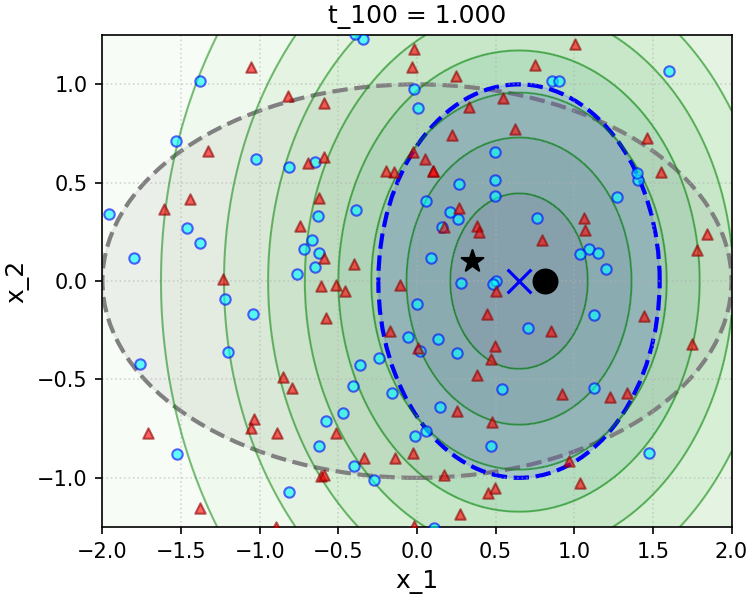
\includegraphics[width=\linewidth]{\toplevelprefix/chapters/chapter6/figs/samples_step_000_t_100_largenoise.png}
    \end{subfigure}
    \hfill
    \begin{subfigure}{0.32\textwidth}
      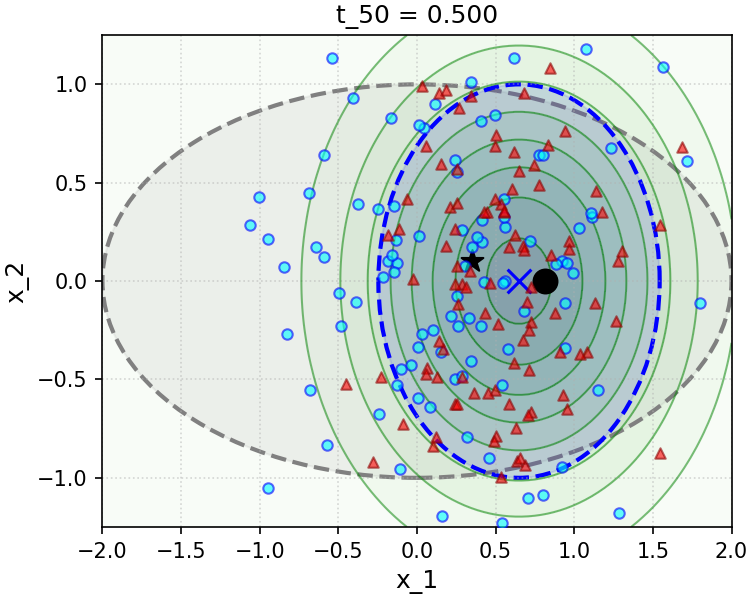
\includegraphics[width=\linewidth]{\toplevelprefix/chapters/chapter6/figs/samples_step_050_t_50_largenoise.png}
    \end{subfigure}
    \hfill
    \begin{subfigure}{0.32\textwidth}
      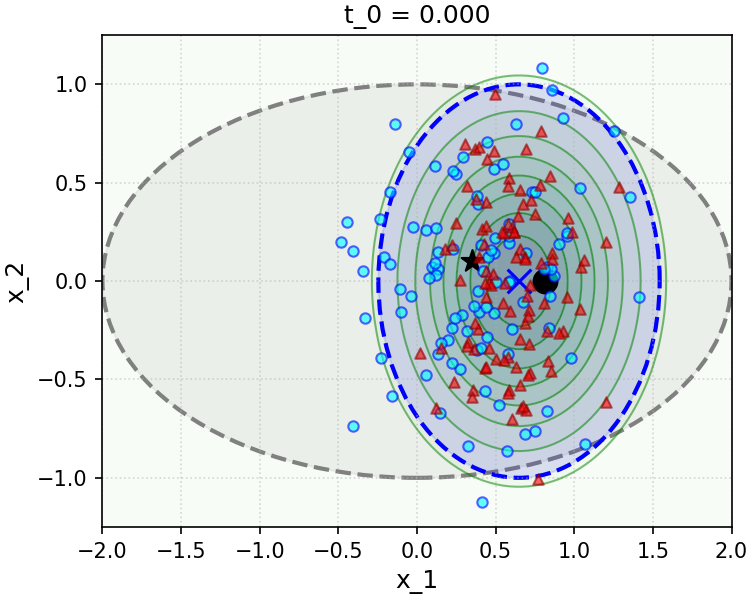
\includegraphics[width=\linewidth]{\toplevelprefix/chapters/chapter6/figs/samples_step_100_t_0_largenoise.png}
    \end{subfigure}

    \vspace{2mm} %

    \begin{subfigure}{0.32\textwidth}
      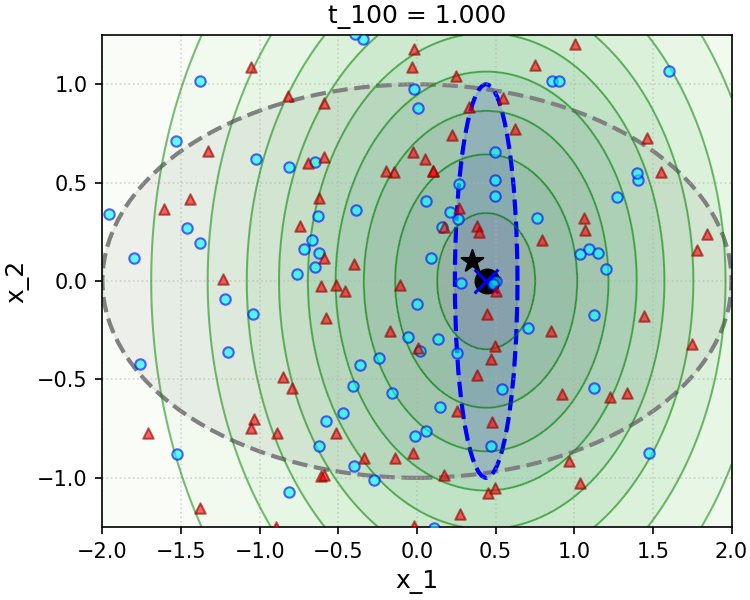
\includegraphics[width=\linewidth]{\toplevelprefix/chapters/chapter6/figs/samples_step_000_t_100_smallnoise.png}
    \end{subfigure}
    \hfill
    \begin{subfigure}{0.32\textwidth}
      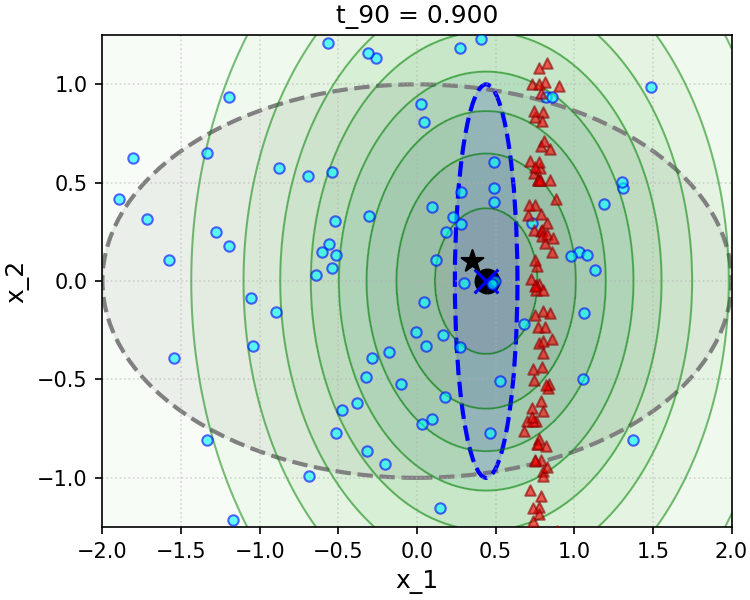
\includegraphics[width=\linewidth]{\toplevelprefix/chapters/chapter6/figs/samples_step_010_t_90_smallnoise.png}
    \end{subfigure}
    \hfill
    \begin{subfigure}{0.32\textwidth}
      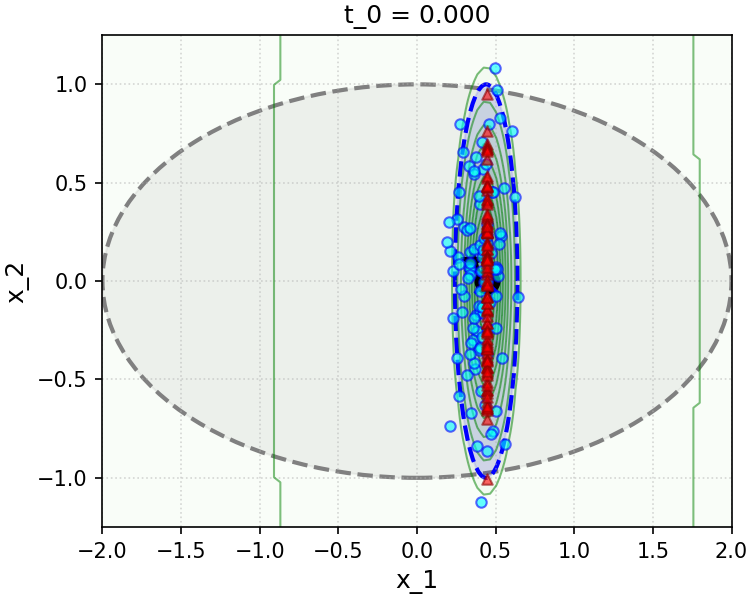
\includegraphics[width=\linewidth]{\toplevelprefix/chapters/chapter6/figs/samples_step_100_t_0_smallnoise.png}
    \end{subfigure}

    \caption{Numerical simulation of the conditional sampling setup
    \eqref{eq:measurement-matching-observation}, with Gaussian data, linear
    measurements, and Gaussian noise. We simulate $D=2$ and $d=1$, with $\vSigma
    = \ve_1 \ve_1^\top + \tfrac{1}{4} \ve_2 \ve_2^\top$, $\vmu = \Zero$, and
    $\vA = \ve_1^\top$. The underlying signal $\vx$ is marked with a black star,
    and the measurement $\vy$ is marked with a black circle.
    Each individual plot corresponds to a different value of sampler time
    $t_{\ell}$, with different rows corresponding to different observation noise
    levels $\sigma^2$.
    In each plot, the covariance matrix of $\vx$ is plotted in gray, the
    posterior covariance matrix and posterior mean of $p_{\vx \mid \vy}$ are
    plotted in blue (with the posterior mean marked by a blue ``x''), and
    contours for $p_{\vx_{t_{\ell}} \mid \vy}$ are drawn in green. The sampler
    hyperparameters are $T=1$, $L=100$, and we draw $100$
    independent samples to initialize the samplers. Samplers are implemented
    with the closed-form denoisers derived in
    \Cref{example:denoising-conditional-gaussian}, with those using the
    approximation
    \eqref{eq:conditional-posterior-measurementmatching-gaussian-case-dps-approx}
    marked with red triangles, and those using the exact conditional posterior
    denoiser marked with blue circles.
    \textbf{Top:} For large observation noise $\sigma = 0.5$, both the exact
    conditional posterior denoiser and the approximate one do a good job of
    converging to the posterior $p_{\vx \mid \vy}$. Sampling time (corresponding
    to time in the ``forward process'', so larger times mean larger noise)
    decreases from left to right.  The convergence dynamics for the exact and
    approximate measurement matching term are similar. \textbf{Bottom:} For
    smaller observation noise $\sigma = 0.1$, the
    approximate measurement matching term leads to extreme bias in the sampler
    (red triangles): samples rapidly converge to an affine subspace
    of points that are consistent, modulo some shrinkage from the posterior mean
    denoiser, with the measured ground truth, and later sampling iterations are
    unable to recover the lost posterior variance along this dimension. Note
    that different times $t_{\ell}$ are plotted in the bottom row, compared to
    the top row, to show the rapid collapse of the approximation to the
    posterior along the measurement dimension.}
    \label{fig:conditional_sampling_computational_gaussian}
  \end{figure}

  \Cref{eq:conditional-posterior-measurementmatching-gaussian-case-dps-approx}
  is, of course, a direct consequence of our calculations above. However, notice
  that if we directly interpret this approximation, it is \textit{ab initio}
  tractable: the likelihood $p_{\vy \mid \vx} = \cN(\vA\vx, \sigma^2 \vI)$ is
  a simple Gaussian distribution centered at the observation, and the
  approximation to the measurement matching term that we arrive at can be
  interpreted as simply evaluating the log-likelihood at the conditional
  expectation $\bE[\vx \mid \vx_t = \vxi]$, then taking gradients with respect
  to $\vxi$ (and backpropagating through the conditional expectation, which is
  given here by \Cref{eq:posterior-denoiser-gaussian-case}).
  Nevertheless, note that the approximation in
  \Cref{eq:conditional-posterior-measurementmatching-gaussian-case-dps-approx}
  requires $t \ll \sqrt{\lambda_{\min}(\vSigma)}$, and that it is never accurate
  in general when this condition does not hold, even in this Gaussian setting.

  To gain insight into the effect of the convenient approximation
  \eqref{eq:conditional-posterior-measurementmatching-gaussian-case-dps-approx},
  we implement and simulate a simple numerical experiment in the Gaussian
  setting in \Cref{fig:conditional_sampling_computational_gaussian}. 
  The sampler we implement is a direct implementation of the simple scheme
  \eqref{eq:denoising-iteration-basic} we have developed in \Cref{ch:compression}
  and recalled above, using the true conditional posterior denoiser, i.e.\
  \Cref{eq:conditional-posterior-denoiser-gaussian-case} (top row of
  \Cref{fig:conditional_sampling_computational_gaussian}), and the 
  convenient approximation to this denoiser made with the decomposition
  \eqref{eq:posterior-sampling-denoiser-decomposition}, the posterior denoiser
  \eqref{eq:posterior-denoiser-gaussian-case}, and the measurement
  matching approximation
  \eqref{eq:conditional-posterior-measurementmatching-gaussian-case-dps-approx}
  (bottom row of \Cref{fig:conditional_sampling_computational_gaussian}).
  We see that even in the simple Gaussian setting, the approximation to the
  measurement matching term we have made is not without its
  drawbacks---specifically, at small noise levels $\sigma^2 \ll 1$, it leads to
  rapid collapse of the variance of the sampling distribution along directions
  that are parallel to the rows of the linear measurement operator $\vA$, which
  cannot be corrected by later iterations of sampling. We can intuit this from
  the approximation
  \eqref{eq:conditional-posterior-measurementmatching-gaussian-case-dps-approx}
  and the definition of the denoising iteration
  \eqref{eq:denoising-iteration-basic}, given
  \Cref{eq:posterior-sampling-denoiser-decomposition}: for $\sigma^2 \ll 1$,
  early steps of sampling effectively take gradient descent steps with a very
  large step size on the likelihood, via
  \Cref{eq:conditional-posterior-measurementmatching-gaussian-case-dps-approx},
  which leads the sampling distribution to get ``stuck'' in a collapsed state.

\end{example}


\Cref{example:denoising-conditional-gaussian} suggests a convenient
approximation for the measurement matching term
\eqref{eq:conditional-posterior-measurementmatching-gaussian-case-dps-approx},
which can be made beyond the Gaussian setting of the example. To
motivate this approximation in greater generality, notice that
by conditional independence of $\vy$ and $\vx_t$ given $\vx$, we can write
\begin{equation}
  p_{\vy \mid \vx_t}(\vnu \mid \vxi)
  =
  \int p_{\vy \mid \vx}(\vnu \mid \vxi') p_{\vx \mid \vx_t}(\vxi' \mid \vxi)
  \odif  \vxi'.
\end{equation}
Formally, when the posterior $p_{\vx\mid \vx_t}$ is a delta function centered at
its mean $\bE[\vx \mid \vx_t=\vxi]$, the approximation
\eqref{eq:conditional-posterior-measurementmatching-gaussian-case-dps-approx} is
exact. More generally, when the posterior $p_{\vx \mid \vx_t}$ is highly
concentrated around its mean, the approximation
\eqref{eq:conditional-posterior-measurementmatching-gaussian-case-dps-approx} is
accurate. This holds, for example, for sufficiently small $t$, which we saw
explicitly in the Gaussian setting of
\Cref{example:denoising-conditional-gaussian}.
Although the numerical simulation in
\Cref{fig:conditional_sampling_computational_gaussian} suggests that this
approximation is not without its caveats in certain regimes, it has proved to be
a reliable baseline in practice, after being proposed by Chung et al.\ as
``Diffusion Posterior Sampling'' (DPS) \cite{chung2023diffusion}.
In addition, there are even principled and generalizable approaches to improve it by
incorporating better estimates of the posterior variance (which turn out to be
exact in the Gaussian setting of \Cref{example:denoising-conditional-gaussian}),
which we discuss further in the end-of-chapter summary. 

Thus, with the DPS approximation, we arrive at the following approximation for
the conditional posterior denoisers $\bE[\vx \mid \vy, \vx_t]$, via
\Cref{eq:posterior-sampling-denoiser-decomposition}:
\begin{equation}
  \bE[ \vx \mid \vx_t=\vxi, \vy=\vnu]
  \approx
  \bE[\vx \mid \vx_t=\vxi] 
  + t^2 \nabla_{\vxi} \log p_{\vy \mid \vx}(\vnu \mid \bE[\vx \mid \vx_t = \vxi]).
  \label{eq:posterior-sampling-denoiser-decomposition-dps}
\end{equation}
And, for a neural network or other model $\bar{\vx}_{\theta}(t, \vxi)$ 
trained as in \Cref{sub:compression_denoising} to approximate the denoisers
$\bE[\vx \mid \vx_t = \vxi]$ for each $t \in [0, T]$, we arrive at the learned
conditional posterior denoisers
\begin{equation}
  \bar{\vx}_{\theta}(t, \vxi, \vnu) 
  = \bar{\vx}_{\theta}(t, \vxi)
  + t^2 \nabla_{\vxi} \log p_{\vy \mid \vx}(\vnu \mid \bar{\vx}_{\theta}(t,
  \vxi)).
  \label{eq:posterior-sampling-denoiser-learned-dps}
\end{equation}
Note that the approximation
\eqref{eq:posterior-sampling-denoiser-decomposition-dps} is  valid for arbitrary
forward models $h$ in the
observation model \eqref{eq:measurement-matching-observation}, including
nonlinear $h$, and even to
arbitrary noise models for which a clean expression for the likelihood $p_{\vy
\mid \vx}$ is known. Indeed, in the case of Gaussian noise, we have
\begin{equation}
  p_{\vy \mid \vx}(\vnu \mid \vxi)
  \propto
  \exp\left(
    -\frac{1}{2\sigma^2} \norm*{ h(\vxi) - \vnu }_2^2
  \right).
\end{equation}
Hence, evaluating the righthand side of
\eqref{eq:posterior-sampling-denoiser-learned-dps}
requires only
\begin{enumerate}
  \item A pretrained denoiser $\bar{\vx}_{\theta}(t, \vxi)$ for the data distribution $p$
    (of $\vx)$, learned as in \Cref{sub:compression_denoising} via
    \Cref{alg:learning_denoiser};
  \item Forward and backward pass access to the forward model $h$ for the
    measurements \eqref{eq:measurement-matching-observation};
  \item A forward and backward pass through $\bar{\vx}_{\theta}(t, \vxi)$, which can be evaluated
    efficiently using (say) backpropagation.
\end{enumerate}

\begin{algorithm}
  \caption{Conditional sampling under measurements
  \eqref{eq:measurement-matching-observation}, with an unconditional denoiser and DPS.}
	\label{alg:iterative_denoising_conditional_DPS}
	\begin{algorithmic}[1]
		\Require{An ordered list of timesteps \(0 \leq t_{0} < \cdots < t_{L} \leq T\) to use for sampling.}
    \Require{An unconditional denoiser \(\bar{\vx}_{\theta} \colon
    \{t_{\ell}\}_{\ell = 1}^{L} \times \R^{D} \to \R^{D}\) for $p_{\vx}$.}
    \Require{Measurement realization $\vnu$ of $\vy$ (\Cref{eq:measurement-matching-observation}) to condition on.}
    \Require{Forward model $h : \bR^D \to \bR^d$ and measurement noise variance
    $\sigma^2 > 0$.}
		\Require{Scale and noise level functions \(\alpha, \sigma \colon \{t_{\ell}\}_{\ell = 0}^{L} \to \R_{\geq 0}\).}
    \Ensure{A sample \(\hat{\vx}\), approximately from \(p_{\vx \mid \vy}\).}
    \Function{DDIMSamplerConditionalDPS}{$\bar{\vx}_{\theta}, \vnu, h, \sigma^2,
    (t_{\ell})_{\ell = 0}^{L}$}
		\State{Initialize \(\hat{\vx}_{t_{L}} \sim\) approximate distribution of \(\vx_{t_{L}}\)} \Comment{VP \(\implies \dNorm(\vzero, \vI)\), VE \(\implies \dNorm(\vzero, t_{L}^{2}\vI)\).}
		\For{\(\ell = L, L - 1, \dots, 1\)}
		\State{Compute
			\begin{equation*}
				\hat{\vx}_{t_{\ell - 1}} \doteq \frac{\sigma_{t_{\ell
        - 1}}}{\sigma_{t_{\ell}}}\hat{\vx}_{t_{\ell}} + \bp{\alpha_{t_{\ell
        - 1}} - \frac{\sigma_{t_{\ell
        - 1}}}{\sigma_{t_{\ell}}}\alpha_{t_{\ell}}}\left(
        \bar{\vx}_{\theta}(t_{\ell}, \hat{\vx}_{t_{\ell}})
        - \frac{\sigma_{t_{\ell}}^2}{2\alpha_{t_\ell}\sigma^2}
        \nabla_{\vxi}\left[ \norm*{h( \bar{\vx}_{\theta}(t_{\ell}, \vxi)
        ) - \vnu}_2^2 \right]\biggl|_{\vxi = \hat{\vx}_{t_{\ell}}}\biggr.
        \right)
			\end{equation*}
		}
		\EndFor
		\State{\Return{\(\hat{\vx}_{t_{0}}\)}}
		\EndFunction
	\end{algorithmic}
\end{algorithm}

Combining this scheme with the basic implementation of unconditional sampling we
developed in \Cref{sub:compression_denoising}, we obtain a practical algorithm for
conditional sampling of the posterior $p_{\vx \mid \vy}$ given measurements
following \eqref{eq:measurement-matching-observation}.
\Cref{alg:iterative_denoising_conditional_DPS} records this scheme
for the case of
Gaussian observation noise with known standard deviation $\sigma$, with minor
modifications to extend to a general noising process, as in
\Cref{eq:gen_additive_gaussian_noise_model} and the surrounding discussion in
\Cref{ch:compression} (our discussion above made the simplifying choices $\alpha_t = 1$, $\sigma_t = t$, and
$t_{\ell} = T\ell / L$, as for \Cref{eq:denoising-iteration-basic} in
\Cref{sub:compression_denoising}).



\subsection{Body Pose Generation Conditioned on Head and Hands}\label{sub:ego-allo}
This type of
conditional estimation or generation problem arises rather naturally in many
practical applications. 
A typical problem of this kind is how to estimate and generate body pose and hand gesture conditioned on a given head pose and egocentric images, as illustrated in Figure \ref{fig:pose-teaser}. This is often the problem we need to solve when one is wearing a head-mounted device such as the Vision Pro from Apple or the Project Aria from Meta. The pose of the whole body and the gesture of the hands need to be inferred so that we can use the information to control virtual objects that the person interacts with.
\begin{figure*}[t]
  \centering
  \includegraphics[width=\linewidth]{\toplevelprefix/chapters/chapter6/figs/pose-teaser.pdf}
    \caption{
A system that estimates human body height, pose, and hand parameters (middle), conditioned on egocentric SLAM poses and images (left). Outputs capture the wearer's actions in the allocentric reference frame of the scene, which we visualize here with 3D reconstructions (right).
  }
  \label{fig:pose-teaser}

\end{figure*}

Notice that in this case, one only has the head pose provided by the device and a very limited field of view for part of one's hands and upper limbs. The pose of the rest of the body needs to be ``inferred'' or ``completed'' based on such partial information. The only way one can estimate the body pose over time is by learning the joint distribution of the head and body pose sequences in advance and then sampling this prior distribution conditioned on the real-time partial inputs. Figure \ref{fig:pose-method} outlines a system called EgoAllo \cite{yi2024egoallo} to solve this problem based on a learned conditional diffusion-denoising model. 
\begin{figure*}[t]
  \centering
  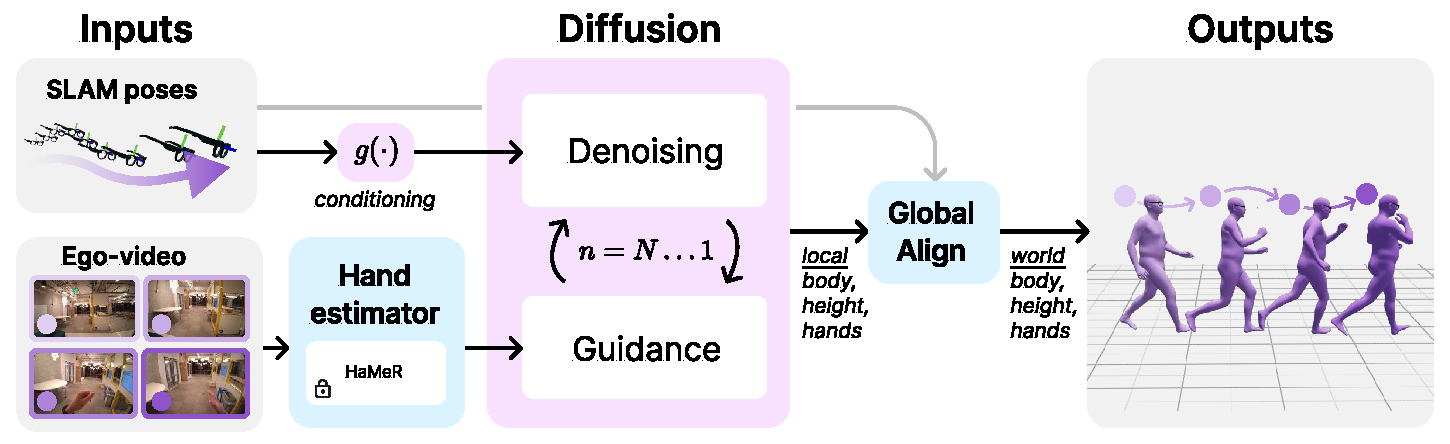
\includegraphics[width=\linewidth]{\toplevelprefix/chapters/chapter6/figs/pose-method.pdf}
\caption{
    \textbf{Overview of technical components of EgoAllo \cite{yi2024egoallo}.}
    A diffusion model is pretrained that can generate body pose sequence based on local body parameters (middle).
    An invariant parameterization $g(\cdot)$ of SLAM poses (left) is used to condition the diffusion model. These can be placed into the global coordinate frame via global alignment to input poses.
    When available, egocentric video is used for hand detection (left) via HaMeR~\cite{pavlakos2023reconstructing}, which can be incorporated into samples via guidance by the generated gesture.
  }
  \label{fig:pose-method}
\end{figure*}


Figure \ref{fig:comparison} compares some ground truth motion sequences with sampled results generated by the EgoAllo. Although the figure shows one result for each input head pose sequence, different runs can generate different body pose sequences that are consistent with the given head pose, all drawing from the distribution of natural full-body motion sequences.
\begin{figure}[t]
\centering
\begin{subfigure}{0.45\textwidth}
  \centering
  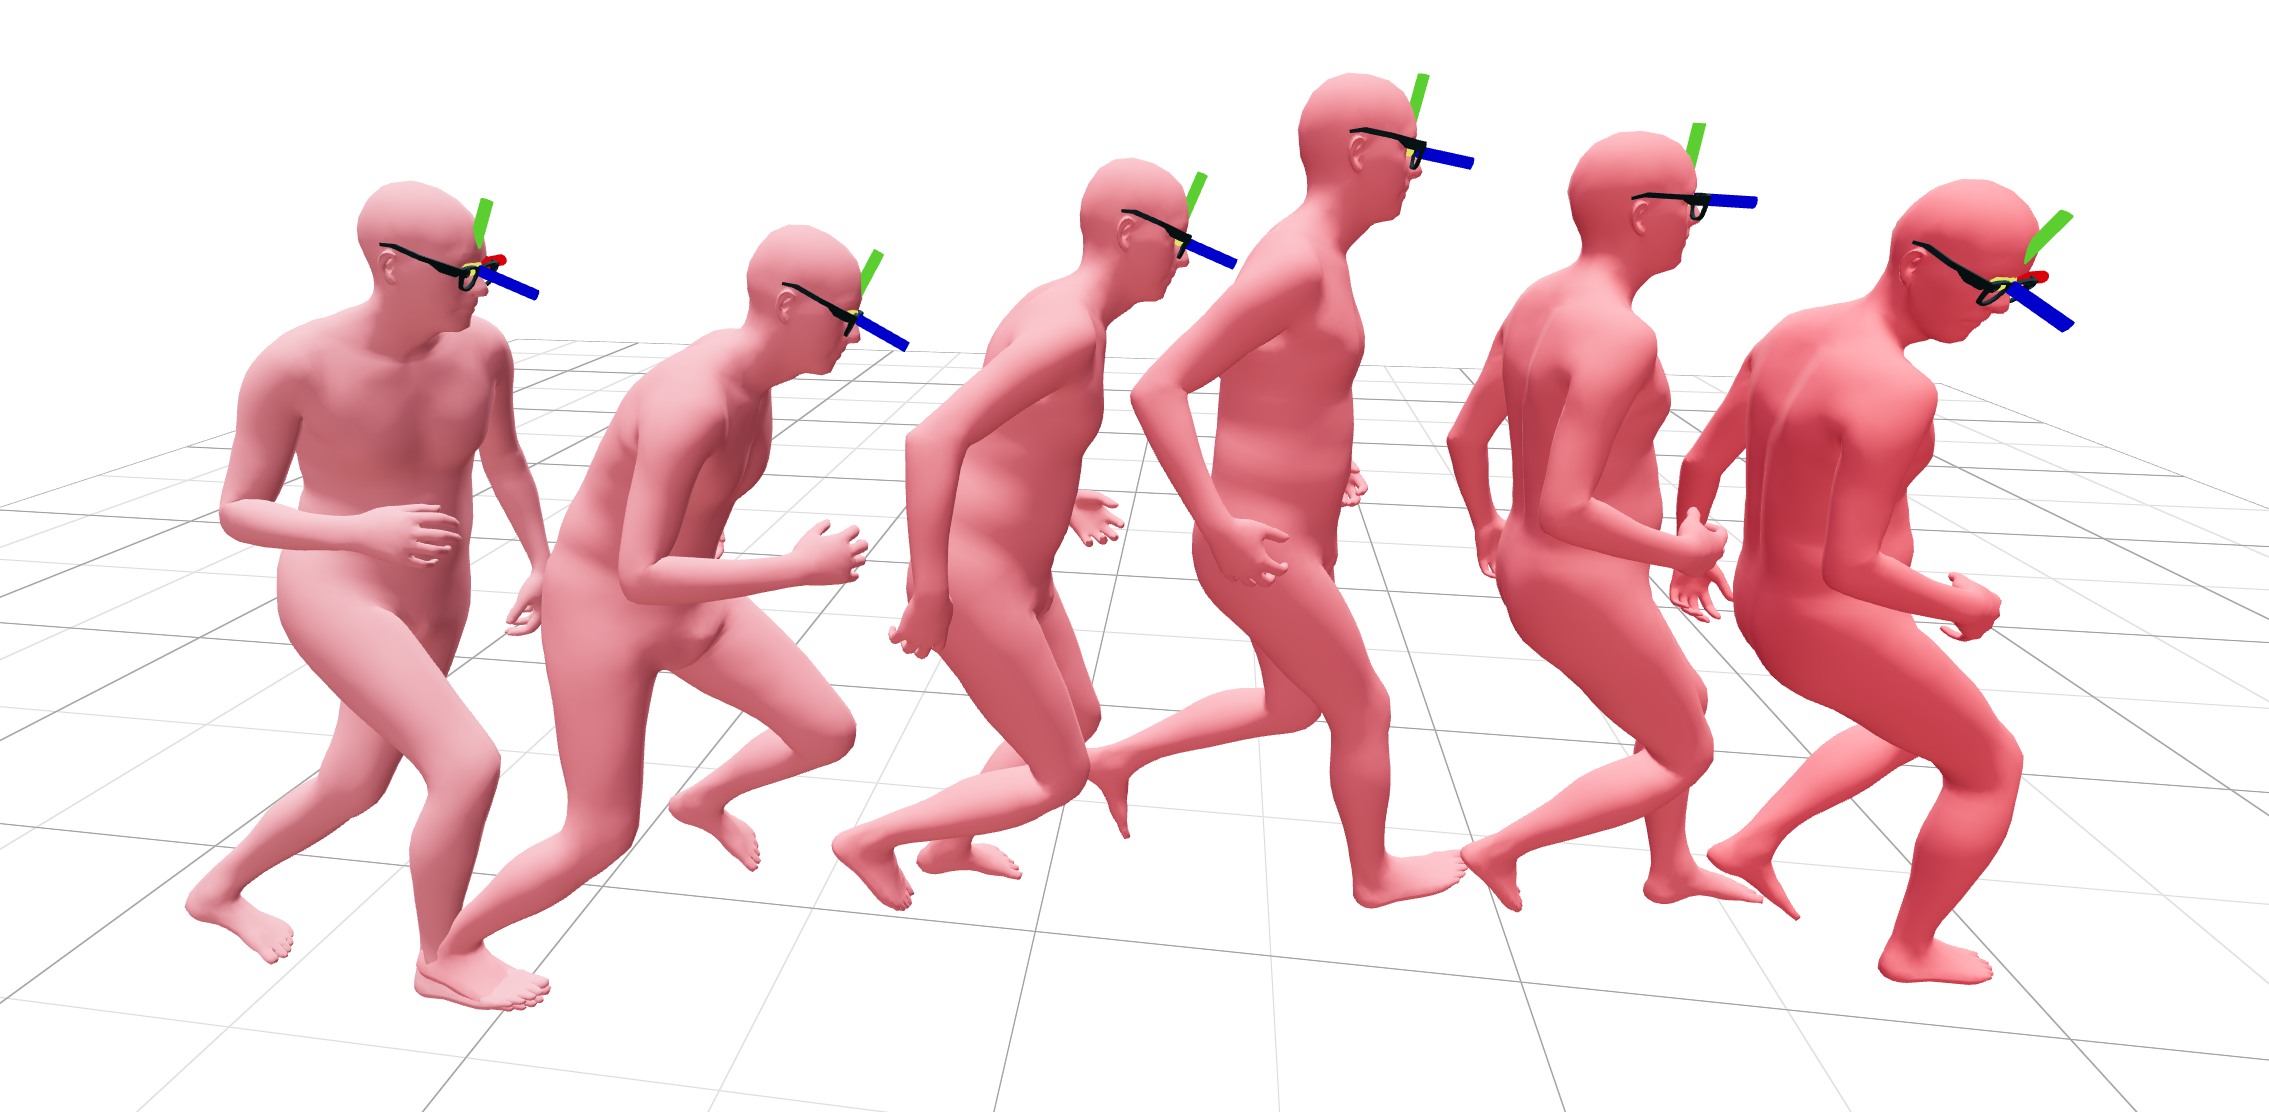
\includegraphics[width=\linewidth]{\toplevelprefix/chapters/chapter6/figs/qual0_gt.png}
  \caption{\centering Ground-truth}
\end{subfigure}
\hfill
\begin{subfigure}{0.45\textwidth}
  \centering
  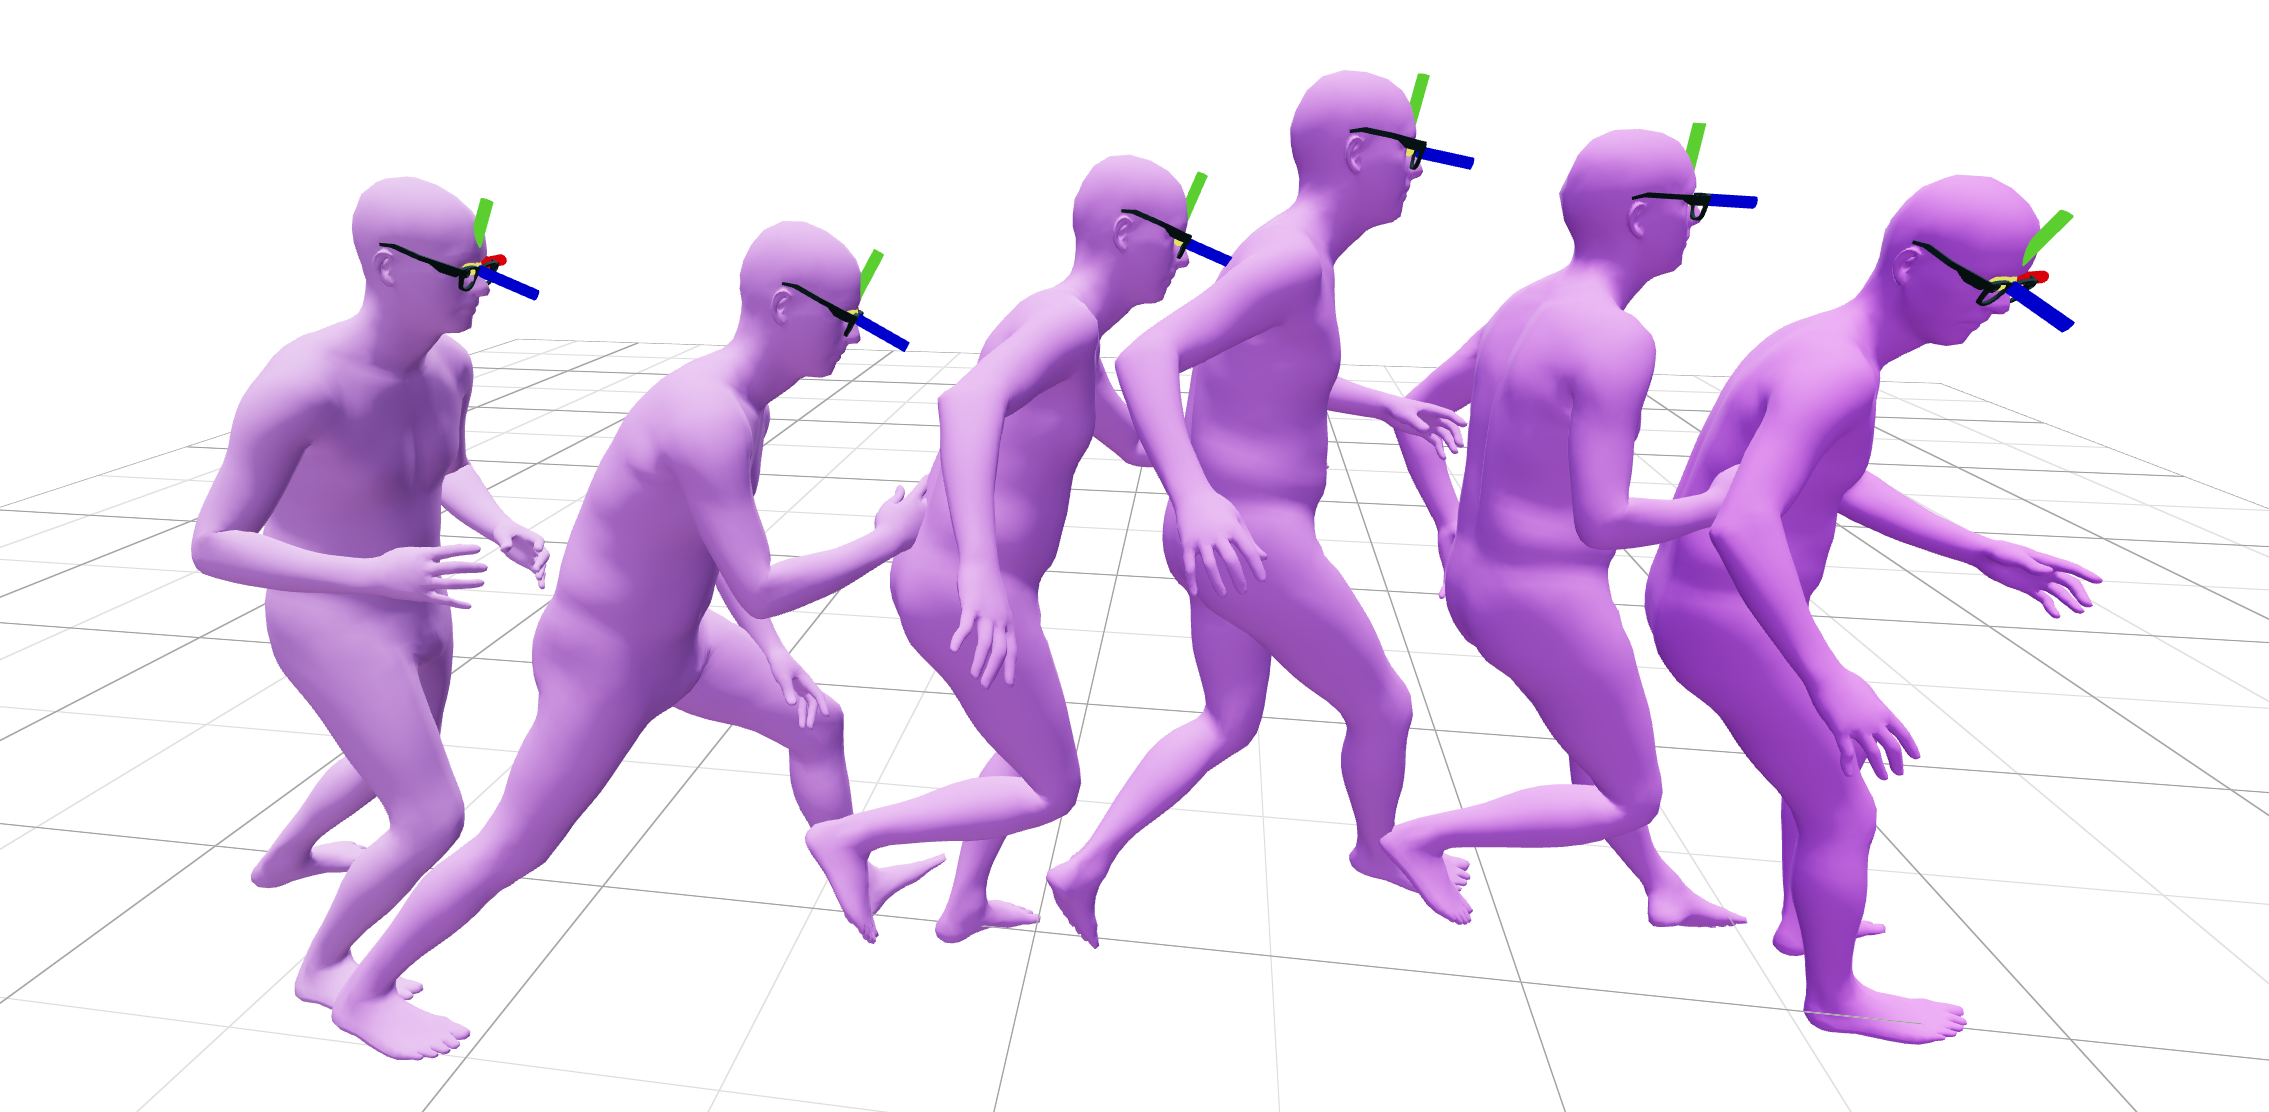
\includegraphics[width=\linewidth]{\toplevelprefix/chapters/chapter6/figs/qual0_ours.png}
  \caption{EgoAllo}
\end{subfigure}

\begin{subfigure}{0.45\textwidth}
  \centering
  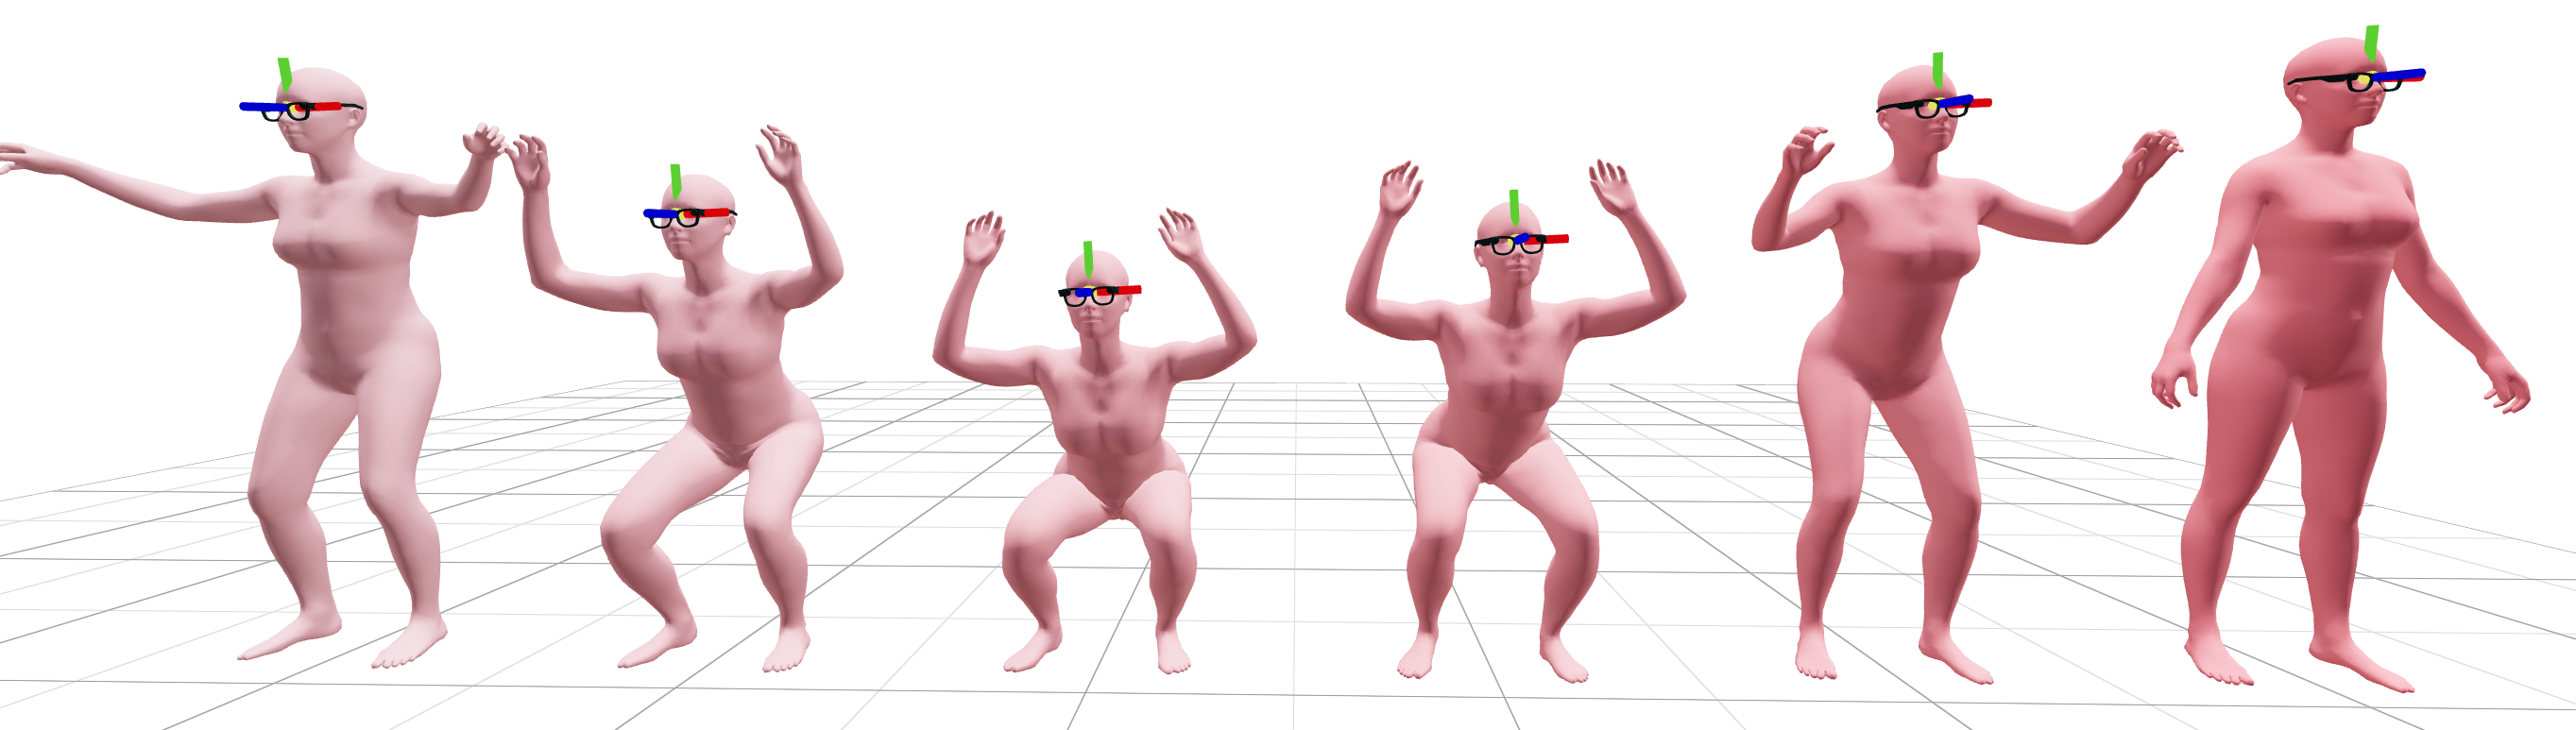
\includegraphics[width=\linewidth]{\toplevelprefix/chapters/chapter6/figs/qual1_gt.png}
  \caption{\centering Ground-truth}
\end{subfigure}
\hfill
\begin{subfigure}{0.45\textwidth}
  \centering
  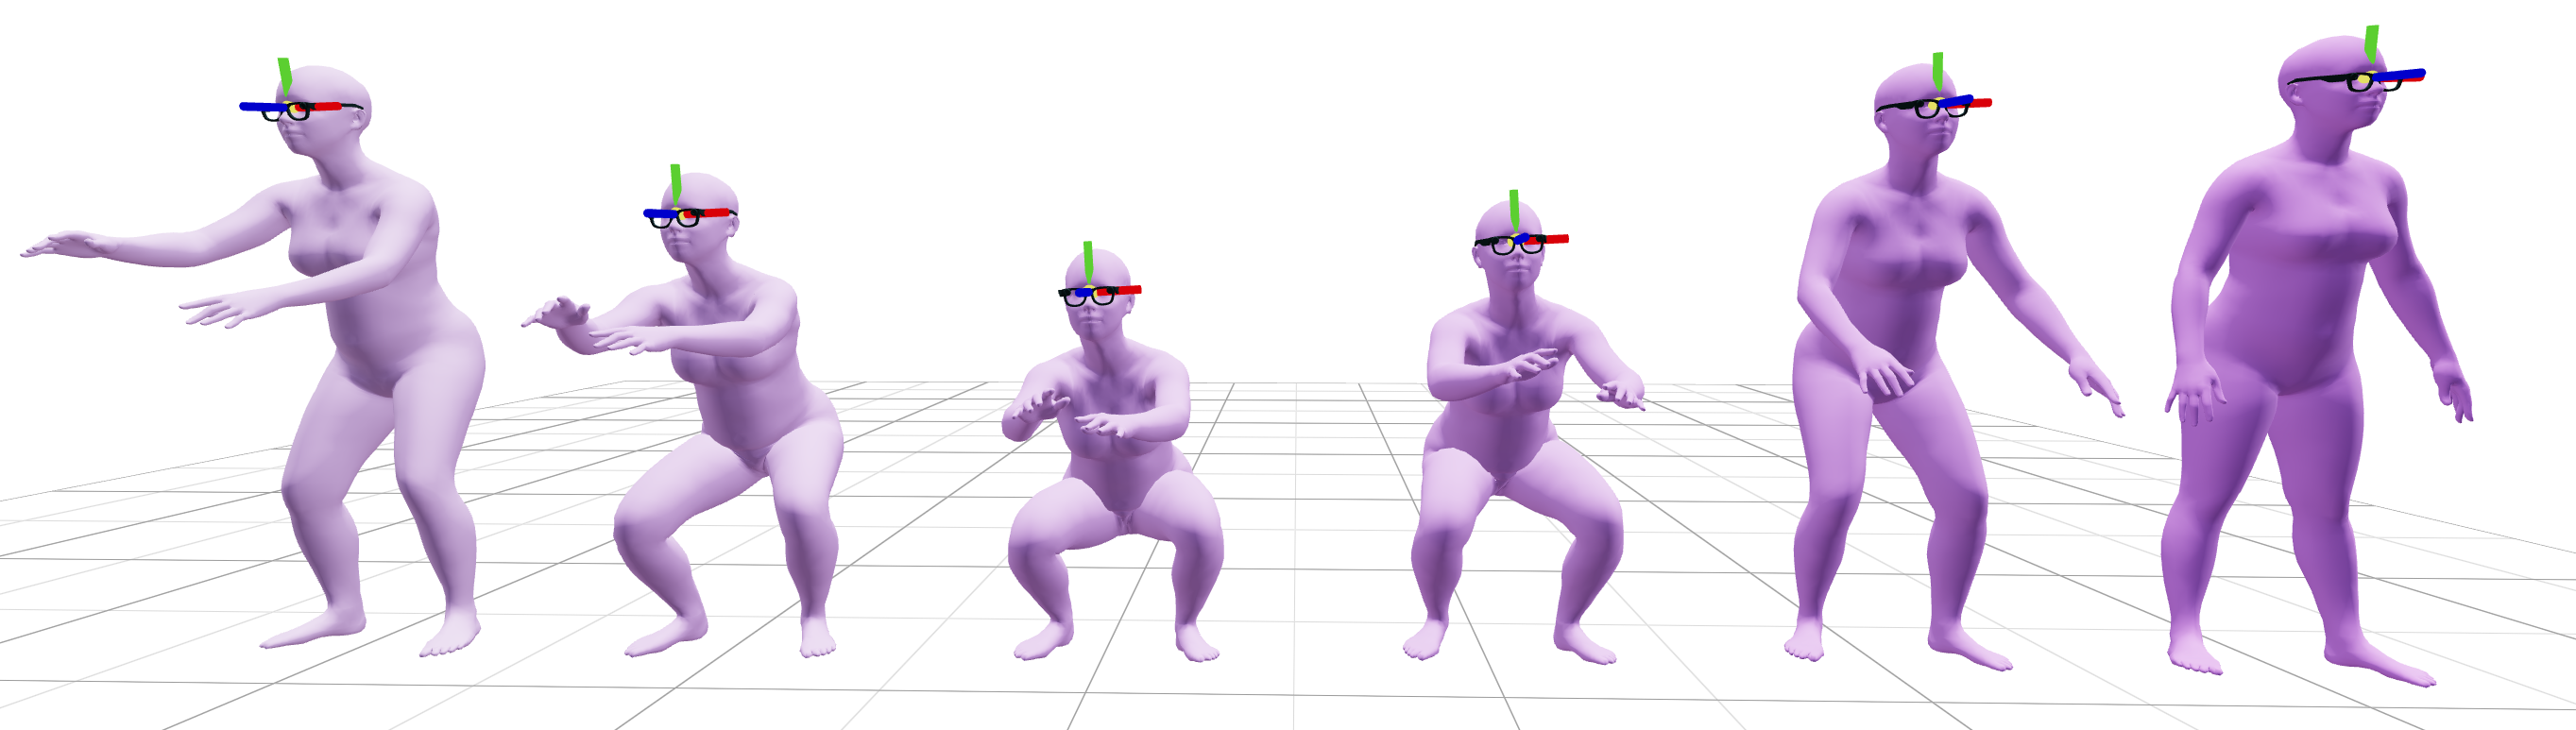
\includegraphics[width=\linewidth]{\toplevelprefix/chapters/chapter6/figs/qual1_ours.png}
  \caption{EgoAllo}
\end{subfigure}

\caption{
\textbf{Egocentric human motion estimation for a running (top) and squatting (bottom) sequence.}
The ground-truth motion is compared with one output from EgoAllo that is consistent with the given head pose sequence. 
}
\label{fig:comparison}
\end{figure}

Strictly speaking, the solution proposed in EgoAllo \cite{yi2024egoallo} does
not enforce measurement matching using the techniques introduced above. Instead
it heuristically enforces the condition by utilizing  the cross-attention
mechanism in a transformer architecture. As we will describe with more precision
in the paired data setting in \Cref{sub:text-cond}, there is reason to believe that the
cross-attention mechanism is in a way approximately realizing the conditional
sampling of the denoising a posteriori. We believe the more principled
techniques introduced here, if properly implemented, can lead to better methods
that further improve the body pose and hand gesture estimation. 

\section{Conditional Inference with Paired Data and Measurements}
In many practical applications, we do not know either the distribution of the data $\x$ of interest or the explicit relationship between the data and certain observed attributes $\y$ of the data. We only have  a (large) set of paired samples $(\X, \Y) = \{ (\x_1, \y_1), \ldots, (\x_N, \y_N) \}$ from which we need to infer the data distribution and a mapping that models their relationship:
\begin{equation}
  h: \x \mapsto \y.
\end{equation}

The problem of image classification can be viewed as one such example. In a sense, the classification problem is to learn an (extremely lossy) compressive encoder for natural images. Say, given a random sample of an image $\x$, we would like to predict its class label $\y$ that best correlates the content in $\x$. We know the distribution of natural images of objects is low-dimensional compared to the dimension of the pixel space. From the previous chapters, we have learned that given sufficient samples, in principle, we can learn a structured low-dimensional representation $\z$ for $\x$ through a learned compressive encoding:
\begin{equation}
    f: \x \mapsto \z. 
\end{equation}
The representation $\z$ can also be viewed as a learned (lossy but structured) code for $\x$. It is rather reasonable to assume that if the class assignment $\y$ truly depends on the low-dimensional structures of $\x$ and the learned code $\z$ truly reflects such structures, $\y$ and $\z$ can be made highly correlated and hence their joint distribution $p(\z, \y)$ should be extremely low-dimensional. Therefore, we may combine the two desired codes $\y$ and $\z$ together and try to learn a combined encoder:
\begin{equation}
    f: \x \mapsto (\z, \y) 
\end{equation}
where the joint distribution of $(\z, \y)$ is highly low-dimensional. 

From our study in previous chapters, the mapping $f$ is usually learned as a sequence of compression or denoising operators in the same space. Hence to leverage such a family of operations, we may introduce an auxiliary vector $\vw$ that can be viewed as an initial random guess of the class label $\y$. In this way, we can learn a compression or denoising mapping:
\begin{equation}\label{eq:classifier-with-class-token}
    f: (\x, \vw) \mapsto (\z, \y)
\end{equation}
within a common space. In fact, the common practice of introducing an auxiliary ``class token'' in the training of a transformer for classification tasks, such as in ViT, can be viewed as learning such a representation by compressing (the coding rate of) given (noisy) samples of $(\x, \vw)$. If the distribution of the data $\x$ is already a mixture of (low-dimensional) Gaussians, the work \cite{wright2008classification} has shown that classification can be done effectively by directly minimizing {\em the (lossy) coding length} associated with the given samples.


\subsection{Class Conditioned Image Generation}\label{sub:cfg} 
While a learned classifier allows us to classify a given image $\x$ to its
corresponding class, we often would like to generate an image of a given class, by
sampling the learned distribution of natural images. To some extent, this can be
viewed as the ``inverse'' problem to image classification. Let $p_{\x}$ denote
the distribution of natural images, say modeled by a diffusion-denoising
process. Given a class label random variable $y \in [K]$ with realization $\nu$, say
an ``Apple'', we would like to sample the conditional distribution $p_{\x \mid
y}(\,\cdot\, \mid \nu)$ to generate an image of an apple:
\begin{equation}
  \hat{\x} \sim p_{\x\mid \y}(\,\cdot\, \mid \vnu).
\end{equation}
We call this {\em class-conditioned image generation}.

In \Cref{sec:conditioned-decoding}, we have seen how to use the denoising-diffusion paradigm for
conditional sampling from the posterior $p_{\vx \mid \vy}$ given
\textit{model-based} measurements $\vy = h(\vx) + \vw$
(\Cref{eq:measurement-matching-observation}), culminating in the
DPS algorithm (\Cref{alg:iterative_denoising_conditional_DPS}). This is a powerful
framework, but it does not apply to the class (or text) conditioned image
generation problem here, where an explicit generative model $h$ for the
observations/attributes $y$ is not available due to the
intractability of analytical modeling. In this section, we will present techniques for extending
conditional sampling to this setting.


Thus, we now assume only that we have access to samples from the joint
distribution of $(\vx, y)$:
\begin{equation}
  (\vx, y) \sim p_{\vx, y}.
\end{equation}
As in the previous section, we define $\vx_t = \alpha_t \vx + \sigma_t \vg$
with $\vg \sim \cN(\Zero, \vI)$ independent of $(\vx, \vy)$, as in
\Cref{eq:gen_additive_gaussian_noise_model} in \Cref{ch:compression},
and we will repeatedly use the notation $\vxi$ to denote realizations of $\vx$
and $\vx_t$.

To proceed, we note that our development of conditional sampling under
measurements $\vy = h(\vx) + \vw$ only explicitly used the
forward model $h$ in making the DPS approximation
\eqref{eq:conditional-posterior-measurementmatching-gaussian-case-dps-approx}.
In particular, the conditional posterior denoiser decomposition
\eqref{eq:posterior-sampling-denoiser-decomposition} \textit{still holds in the
paired data setting}, by virtue of Bayes' rule
and conditional independence of $\vy$ and $\vx_t$ given $\vx$ (recall
\Cref{fig:posterior-sampling-cds}). Thus we can still write in the paired
data setting
\begin{equation}\label{eq:conditional-denoising-mmse-denoiser-paired-data}
  \bE[ \vx \mid \vx_t=\vxi, y=\nu]
  =
  \bE[\vx \mid \vx_t=\vxi] 
  + \frac{\sigma_t^2}{\alpha_t} 
  \nabla_{\vxi}\log p_{y \mid \vx_t}(\nu\mid \vxi).
\end{equation}
A natural ideal is then to directly implement the likelihood correction term in
\eqref{eq:conditional-denoising-mmse-denoiser-paired-data} using a deep network
$f_{\theta_{\mathrm{c}}}$ with parameters $\theta_{\mathrm{c}}$, as in
\Cref{eq:classifier-with-class-token}: 
\begin{equation}
  f_{\theta_{\mathrm{c}}} : (t, \vx_t) \mapsto \softmax(\vW_{\mathrm{head}}
  \vz(t, \vx_t)).
\end{equation}
This expression combines the final representations $\vz(t, \vx_t)$ (which also depend on
$\theta_{\mathrm{c}}$) of the noisy inputs
$\vx_t$ with a classification head $\vW_{\mathrm{head}} \in \bR^{K \times d}$, which maps the
representations to a probability distribution over the $K$ possible classes.
As is common in practice, it also takes the time $t$ in the noising process as
input.
Thus, with appropriate training, it provides an approximation to the log-likelihood
$\log p_{y \mid \vx_t}$, and differentiating $\log f_{\theta_{\mathrm{c}}}$ with
respect to its input $\vx_t$
allows an approximation to the second term in
\Cref{eq:conditional-denoising-mmse-denoiser-paired-data}:
\begin{equation}\label{eq:conditional-denoising-mmse-denoiser-paired-data-approx}
  \bar{\vx}_{\theta}^{\mathrm{naive}}(t, \vx_t, y)
  =
  \bar{\vx}_{\theta_{\mathrm{d}}}(t, \vx_t)
  + \frac{\sigma_t^2}{\alpha_t}
  \nabla_{\vx_t}
  \ip*{
    \log f_{\theta_{\mathrm{c}}}(t, \vx_t)
  }{
    \ve_{y}
  }
\end{equation}
where, as usual, we approximate the first term in
\Cref{eq:conditional-denoising-mmse-denoiser-paired-data} via a learned
unconditional denoiser for $\vx_t$ with parameters $\theta_{\mathrm{d}}$, and
where we write $\ve_k$ for $k \in [K]$ to denote the $k$-th canonical basis
vector for $\R^K$ (i.e., the vector with
a one in the $k$-th position, and zeros elsewhere).
The reader should note that the conditional denoiser $\bar{\vx}_{\theta}$
requires two separate training runs, with separate losses: one for the
classifier parameters $\theta_{\mathrm{c}}$, on a classification
loss,\footnote{In \Cref{ch:applications}, we review the process of training such
a classifier in full detail.} and one for the denoiser parameters
$\theta_{\mathrm{d}}$, on a denoising loss. Such an approach to conditional
sampling was already recognized and exploited to perform conditional sampling in
pioneering early works on diffusion models, notably those by
\citet{Sohl-Dickstein2015} and by \citet{song2020score}.


However, this straightforward methodology has two key drawbacks (which is why we
label it as ``naive''). The first is
that, empirically, such a trained deep network classifier frequently does not
provide a strong enough guidance signal (in
\Cref{eq:conditional-denoising-mmse-denoiser-paired-data}) to ensure that
generated samples reflect the conditioning information $y$. This was first
emphasized by \citet{Dhariwal2021-hg}, who noted that in the setting of
class-conditional ImageNet generation, the learned deep network
classifier's probability outputs for the class $y$ being conditioned on were
frequently around
$0.5$---large enough to be the dominant class, but not large enough to provide
a strong guidance signal---and that upon inspection, generations were not
consistent with the conditioning class $y$. \citet{Dhariwal2021-hg} proposed to
address this heuristically by incorporating an ``inverse temperature''
hyperparameter $\gamma > 0$
into the definition of the naive conditional denoiser
\eqref{eq:conditional-denoising-mmse-denoiser-paired-data-approx}, referring to the
resulting conditional denoiser as having incorporated ``classifier guidance''
(CG):
\begin{equation}\label{eq:conditional-denoising-mmse-denoiser-paired-data-approx-cg}
  \bar{\vx}_{\theta}^{\mathrm{CG}}(t, \vx_t, y)
  =
  \bar{\vx}_{\theta_{\mathrm{d}}}(t, \vx_t)
  + \gamma\frac{\sigma_t^2}{\alpha_t}
  \nabla_{\vx_t}
  \ip*{
    \log f_{\theta_{\mathrm{c}}}(t, \vx_t)
  }{
    \ve_{y}
  }
\end{equation}
with the case $\gamma = 1$ coinciding with
\eqref{eq:conditional-denoising-mmse-denoiser-paired-data-approx}.
\citet{Dhariwal2021-hg} found that a setting $\gamma > 1$ performed best empirically.
One possible interpretation for this is as follows: note that, in the context of
the \textit{true} likelihood term
\Cref{eq:conditional-denoising-mmse-denoiser-paired-data}, scaling by $\gamma$
gives equivalently
\begin{align}
  \gamma\frac{\sigma_t^2}{\alpha_t} \nabla_{\vxi}\log p_{\vy \mid \vx_t}(\vnu\mid
  \vxi)
  &=
  \frac{\sigma_t^2}{\alpha_t} \nabla_{\vxi}\log \left(
  p_{\vy \mid \vx_t}(\vnu\mid \vxi)^\gamma
  \right), %
\end{align}
which suggests the natural interpretation of the parameter $\gamma$ performing
(inverse) \textit{temperature scaling} on the likelihood
$p_{\vy \mid \vx_t}$, which is precise if we consider the renormalized
distribution 
$ { p_{\vy \mid \vx_t}(\vnu\mid \vxi)^\gamma } / { \int p_{\vy \mid \vx_t}(\vnu'\mid
\vxi)^\gamma \odif \vnu' } $.
However, note that this \textit{is not} a rigorous interpretation in the context
of \Cref{eq:conditional-denoising-mmse-denoiser-paired-data}, because the
gradients are taken with respect to $\vxi$, and the normalization constant in
the temperature-scaled distribution is in general a function of $\vxi$.
Instead, the parameter $\gamma$ should simply be understood as amplifying large
values of the deep network classifier's output probabilities
$f_{\theta_{\mathrm{c}}}(t, \vx_t)$ \textit{relative to} smaller ones,
which effectively amplifies the guidance signal provided in cases where the deep
network $f$ assigns it the largest probability among the $K$ classes.


Nevertheless, classifier guidance does not address the second key drawback of
the naive methodology: it is both cumbersome and wasteful to have to
train an auxiliary classifier $f_{\theta_{\mathrm{c}}}$ in addition to the unconditional
denoiser $\bar{\vx}_{\theta_{\mathrm{d}}}$, given
that it is not possible to directly adapt a pretrained classifier
due to the need for it to work well on noisy inputs $\vx_t$ and incorporate
other empirically-motivated architecture modifications.
In particular, \citet{Dhariwal2021-hg} found that it was necessary to explicitly
design the architecture of the deep network implementing the classifier to match
that of the denoiser.
Moreover, from a purely practical perspective---trying to obtain the best
possible performance from the resulting sampler---the best-performing
configuration of classifier guidance-based sampling departs even further from
the idealized and conceptually sound framework we have presented above.
To obtain the best performance, \citet{Dhariwal2021-hg} found it
necessary to provide the class label $y$ as an additional input to the denoiser
$\bar{\vx}_{\theta_{\mathrm{d}}}$. As a result, the idealized classifier-guided
denoiser \eqref{eq:conditional-denoising-mmse-denoiser-paired-data-approx-cg},
derived by \citet{Dhariwal2021-hg} as we have done above from the conditional
posterior denoiser decomposition
\eqref{eq:conditional-denoising-mmse-denoiser-paired-data}, is not exactly
reflective of the best-performing denoiser in practice---such a denoiser
actually combines a \textit{conditional} denoiser for $\vx_t$ given $y$ with an
additional guidance signal from an auxiliary classifier!

This state of affairs, empirically motivated as it is, led \citet{Ho2022-ry} in
subsequent work to propose a more empirically pragmatic methodology, known as
classifier-free guidance (CFG). Instead of representing the conditional denoiser
\eqref{eq:conditional-denoising-mmse-denoiser-paired-data} as a weighted sum
of an unconditional denoiser for $\vx_t$ with a log-likelihood correction term
(with possibly modified weights, as in classifier guidance), they accept the
apparent necessity of training a conditional denoiser for $\vx_t$ given $y$, as
demonstrated by the experimental results of \citet{Dhariwal2021-hg}, and replace 
the log-likelihood gradient term with a correctly-weighted sum of this
conditional denoiser with an \textit{unconditional} denoiser for $\vx$ given
$\vx_t$.\footnote{That said, \textcite{Ho2022-ry} actually proposed to use
a different weighting than what we present here, based on the fact that
\textcite{Dhariwal2021-hg} heuristically replaced the unconditional denoiser in
\eqref{eq:conditional-denoising-mmse-denoiser-paired-data} with
a conditional denoiser. In fact, the weighting we derive and present here
reflects modern practice, and in particular is used in state-of-the-art
diffusion models such as Stable Diffusion 3.5
\cite{DBLP:conf/icml/EsserKBEMSLLSBP24}.} To see how this structure arises, we
begin with an `idealized' version of the classifier guidance denoiser
$\bar{\vx}_{\theta}^{\mathrm{CG}}$ defined in
\eqref{eq:conditional-denoising-mmse-denoiser-paired-data-approx-cg},
for which the denoiser $\bar{\vx}_{\theta_{\mathrm{d}}}$ and the classifier
$f_{\theta_{\mathrm{c}}}$ perfectly approximate their targets, via
\eqref{eq:conditional-denoising-mmse-denoiser-paired-data}:
\begin{equation}\label{eq:conditional-denoising-mmse-denoiser-paired-data-exact-cg}
  \bar{\vx}_{\theta}^{\mathrm{CG,\,ideal}}(t, \vxi, \nu)
  =
  \bE[\vx \mid \vx_t=\vxi]
  + \gamma\frac{\sigma_t^2}{\alpha_t}
  \nabla_{\vxi}\log p_{y \mid \vx_t}(\nu\mid \vxi).
\end{equation}
We then use Bayes' rule, in the form
\begin{equation}
  \log p_{y \mid \vx_t}
  =
  \log p_{\vx_t \mid y} + \log p_{y} - \log p_{\vx_t},
\end{equation}
together with Tweedie's formula (\Cref{thm:tweedie}, modified as in
\Cref{eq:gen_tweedie}) to convert between score functions and denoisers,
to obtain
\begin{align*}
  \bar{\vx}_{\theta}^{\mathrm{CG,\,ideal}}(t, \vxi, \nu)
  &=
  \frac{1}{\alpha_t} \vxi 
  + (1-\gamma) \frac{\sigma_t^2}{\alpha_t} 
  \nabla_{\vxi}\log p_{\vx_t}(\vxi)
  + \gamma \frac{\sigma_t^2}{\alpha_t} 
  \nabla_{\vxi}\log p_{\vx_t \mid y}(\vxi \mid \nu)
  \\
  &=
  (1 - \gamma) \bE[\vx \mid \vx_t=\vxi]
  +
  \gamma \bE[\vx \mid \vx_t=\vxi, y=\nu],
  \labelthis\label{eq:ideal-cfg-denoiser}
\end{align*}
where in the last line, we apply
\Cref{eq:conditional-denoising-conditioning-order-irrelevant}.
Now, \Cref{eq:ideal-cfg-denoiser} suggests a natural approximation strategy: we
combine a learned unconditional denoiser for $\vx$ given $\vx_t$, as previously,
with a learned \textit{conditional} denoiser for $\vx$ given $\vx_t$ and $y$.


However, following \textcite{Ho2022-ry} and the common practice of training deep network
denoisers, it is standard to use the \textit{same} deep network to represent
both the conditional and unconditional denoisers by introducing an additional
label, which we will denote by $\varnothing$, to denote the ``unconditional''
case.
This leads to the form of the CFG denoiser:
\begin{equation}\label{eq:conditional-denoising-mmse-denoiser-paired-data-approx-cfg}
  \bar{\vx}_{\theta}^{\mathrm{CFG}}(t, \vx_t, y)
  =
  (1 - \gamma) \bar{\vx}_{\theta}(t, \vx_t, \varnothing)
  +
  \gamma \bar{\vx}_{\theta}(t, \vx_t, y).
\end{equation}
To train a denoiser $\bar{\vx}_{\theta}(t, \vx_t, y^+)$ for use with
classifier-free guidance sampling, where $y^+ \in
\set{1, \dots, K, \varnothing}$, we proceed almost identically to the
unconditional training procedure in \Cref{alg:learning_denoiser}, but with two
modifications:
\begin{enumerate}
  \item When we sample from the dataset, we sample a pair $(\vx, y)$ rather than
    just a sample $\vx$.
  \item Every time we sample a pair from the dataset, we sample the augmented
    label $y^+$ via
    \begin{equation}
      y^+ = \begin{cases}
        \varnothing & \text{with probability } p_{\mathrm{uncond}}; \\
        y & \text{else}.
      \end{cases}
    \end{equation}
    Here, $p_{\mathrm{uncond}} \in [0, 1]$ is a new hyperparameter.
    This can be viewed as a form of dropout \cite{srivastava2014dropout}.
\end{enumerate}
In this way, we train a conditional denoiser suitable for use in classifier-free
guidance sampling. We summarize the overall sampling process for
class-conditioned sampling with classifier-free guidance in
\Cref{alg:iterative_denoising_conditional_CFG}.


\begin{algorithm}
  \caption{Conditional sampling with classification data, using class-conditioned denoiser.}
	\label{alg:iterative_denoising_conditional_CFG}
	\begin{algorithmic}[1]
		\Require{An ordered list of timesteps \(0 \leq t_{0} < \cdots < t_{L} \leq T\) to use for sampling.}
    \Require{Class label $\nu \in \set{1, \dots, K}$ to condition on.}
    \Require{A denoiser \(\bar{\vx}_{\theta} \colon
    \{t_{\ell}\}_{\ell = 1}^{L} \times \R^{D} \times \set{1, \dots, K,
    \varnothing} \to \R^{D}\) for $p_{\vx \mid y}$ and $p_{\vx}$ (input $\varnothing$ for
    $p_{\vx}$).}
		\Require{Scale and noise level functions \(\alpha, \sigma \colon \{t_{\ell}\}_{\ell = 0}^{L} \to \R_{\geq 0}\).}
    \Require{Guidance strength $\gamma \geq 0$ ($\gamma > 1$ preferred for
    performance).}
    \Ensure{A sample \(\hat{\vx}\), approximately from \(p_{\vx \mid y}(\,\cdot\,
    \mid \nu)\).}
    \Function{DDIMSamplerConditionalCFG}{$\bar{\vx}_{\theta}, \nu, \gamma,
    (t_{\ell})_{\ell = 0}^{L}$}
		\State{Initialize \(\hat{\vx}_{t_{L}} \sim\) approximate distribution of \(\vx_{t_{L}}\)} \Comment{VP \(\implies \dNorm(\vzero, \vI)\), VE \(\implies \dNorm(\vzero, t_{L}^{2}\vI)\).}
		\For{\(\ell = L, L - 1, \dots, 1\)}
		\State{Compute
			\begin{equation*}
				\hat{\vx}_{t_{\ell - 1}} \doteq \frac{\sigma_{t_{\ell
        - 1}}}{\sigma_{t_{\ell}}}\hat{\vx}_{t_{\ell}} + \bp{\alpha_{t_{\ell
        - 1}} - \frac{\sigma_{t_{\ell
        - 1}}}{\sigma_{t_{\ell}}}\alpha_{t_{\ell}}}\bigl(
        (1 - \gamma) \bar{\vx}_{\theta}(t_{\ell}, \hat{\vx}_{t_{\ell}}, \varnothing)
        + \gamma \bar{\vx}_{\theta}(t_{\ell}, \hat{\vx}_{t_{\ell}}, \nu)
        \bigr)
			\end{equation*}
		}
		\EndFor
		\State{\Return{\(\hat{\vx}_{t_{0}}\)}}
		\EndFunction
	\end{algorithmic}
\end{algorithm}

\textcite{Ho2022-ry} reports strong empirical performance for class-conditional
image generation with classifier-free guidance, and it has become a mainstay of
the largest-scale practical diffusion models, such as Stable Diffusion
\cite{rombach2022high} and its derivatives.
At the same time, its derivation is rather opaque and empirically motivated,
giving little insight into the mechanisms behind its strong performance.
A number of theoretical works have studied this, providing explanations for some
parts of the overall CFG methodology
\cite{Bradley2024-jg,Li2025-li,Wu2024-js}---itself encompassing denoiser
parameterization and training, as well as configuration of the guidance strength
and performance at sampling time.
Below, we will give an interpretation in the simplifying setting
of a Gaussian mixture model data distribution and denoiser, which will
demonstrate an insight into the \textit{parameterization} of the denoiser in the presence of
such low-dimensional structures.


\begin{example}\label{example:denoising-gaussian-mixture-cfg}
  Let us recall the low-rank mixture of Gaussians data generating process we studied in
  \Cref{example:denoising_gaussian_mixture} (and specifically, the form in
  \Cref{eq:MoG1}). Given $K \in \bN$ classes, we assume that
  \begin{equation}\label{eq:MoG1-ch6}
    \vx \sim \frac{1}{K}\sum_{k = 1}^{K}\dNorm(\vzero, \vU_{k}\vU_{k}^{\top}),
  \end{equation}
  where each \(\vU_{k} \in \O(D, P) \subseteq \R^{D \times P}\) is a matrix with
  orthogonal columns, and $P \ll D$.
  Moreover, we assume that the class label $y \in [K]$ is a deterministic
  function of $\vx$ mapping an example to its corresponding mixture component.
  Applying the analysis in \Cref{example:denoising_gaussian_mixture} (and the
  subsequent analysis of the low-rank case, culminating in
  \Cref{eq:gmm_lowrank_denoiser}), we obtain for the class-conditional optimal
  denoisers
  \begin{equation}\label{eq:gmm_lowrank_denoiser-ch6-classcond}
    \bE[ \vx \mid \vx_t = \vxi, y = \nu ]
    = \frac{1}{1 + t^{2}}
    \vU_{\nu}\vU_{\nu}^{\top}\vxi
  \end{equation}
  for each $\nu \in [K]$, and for the optimal unconditional denoiser, we obtain
  \begin{equation}\label{eq:gmm_lowrank_denoiser-ch6-uncond}
    \bE[ \vx \mid \vx_t = \vxi ]
    = \frac{1}{1 + t^{2}}\sum_{k = 1}^{K}\frac{\exp\rp{\frac{1}{2t^{2}(1 + t^{2})}\norm{\vU_{k}^{\top}\vxi}_{2}^{2}}}{\sum_{i = 1}^{K}\exp\rp{\frac{1}{2t^{2}(1 + t^{2})}\norm{\vU_{i}^{\top}\vxi}_{2}^{2}}}\vU_{k}\vU_{k}^{\top}\vxi.
  \end{equation}
  As a result, we can express the CFG denoiser with guidance strength $\gamma
  > 1$ as
  \begin{equation}\label{eq:cfg-denoiser-mog-low-rank}
    \bar{\vx}^{\mathrm{CFG,\,ideal}}(t, \vx_t, y)
    =
    \frac{1}{1 + t^{2}}
    \left(
    (1 - \gamma) 
    \sum_{k = 1}^{K}\frac{\exp\rp{\frac{1}{2t^{2}(1
    + t^{2})}\norm{\vU_{k}^{\top}\vx_t}_{2}^{2}}}{\sum_{i
    = 1}^{K}\exp\rp{\frac{1}{2t^{2}(1
    + t^{2})}\norm{\vU_{i}^{\top}\vx_t}_{2}^{2}}}\vU_{k}\vU_{k}^{\top}
    +
    \gamma 
    \vU_{y}\vU_{y}^{\top}
    \right)
    \vx_t.
  \end{equation}
  This denoiser has a simple, interpretable form. The first term, corresponding
  to the unconditional denoiser, performs denoising of the signal $\vx_t$
  against an average of the denoisers associated with each subspace, weighted by
  how correlated $\vx_t$ is with each subspace. The second term, corresponding to
  the conditional denoiser, simply performs denoising with the conditioning
  class's denoiser. The CFG scheme further averages these two denoisers:
  the effect can be gleaned from the refactoring
  \begin{equation}\label{eq:cfg-denoiser-mog-low-rank-2}
    \begin{split}
      \bar{\vx}^{\mathrm{CFG,\,ideal}}(t, \vx_t, y)
      =
      \frac{1}{1 + t^{2}}
      &\Biggl(
      \left[\gamma + (1 - \gamma) 
      \frac{\exp\rp{\frac{1}{2t^{2}(1
      + t^{2})}\norm{\vU_{y}^{\top}\vx_t}_{2}^{2}}}{\sum_{i
      = 1}^{K}\exp\rp{\frac{1}{2t^{2}(1
      + t^{2})}\norm{\vU_{i}^{\top}\vx_t}_{2}^{2}}}
      \right]
      \vU_{y}\vU_{y}^{\top}
      \\
      &\quad+
      (1 - \gamma) 
      \sum_{k \neq y}\frac{\exp\rp{\frac{1}{2t^{2}(1
      + t^{2})}\norm{\vU_{k}^{\top}\vx_t}_{2}^{2}}}{\sum_{i
      = 1}^{K}\exp\rp{\frac{1}{2t^{2}(1
      + t^{2})}\norm{\vU_{i}^{\top}\vx_t}_{2}^{2}}}\vU_{k}\vU_{k}^{\top}
      \Biggr)
      \vx_t.
    \end{split}
  \end{equation}
  We have
  \begin{equation}
    \sum_{k=1}^K
    \frac{\exp\rp{\frac{1}{2t^{2}(1
    + t^{2})}\norm{\vU_{k}^{\top}\vx_t}_{2}^{2}}}{\sum_{i
    = 1}^{K}\exp\rp{\frac{1}{2t^{2}(1
    + t^{2})}\norm{\vU_{i}^{\top}\vx_t}_{2}^{2}}}
    = 1,
  \end{equation}
  and each summand is nonnegative, hence also bounded above by $1$.
  So we can conclude two regimes for the terms in
  \Cref{eq:cfg-denoiser-mog-low-rank-2}: 
  \begin{enumerate}
    \item \textbf{Well-correlated regime:} If $\vx_t$ correlates well with
      $\vU_y$, then the normalized weight corresponding to the $k=y$ summand in
      the unconditional denoiser is near to $1$. 
      Then 
      \begin{equation}
        \gamma + (1 - \gamma) 
      \frac{\exp\rp{\frac{1}{2t^{2}(1
      + t^{2})}\norm{\vU_{y}^{\top}\vx_t}_{2}^{2}}}{\sum_{i
      = 1}^{K}\exp\rp{\frac{1}{2t^{2}(1
      + t^{2})}\norm{\vU_{i}^{\top}\vx_t}_{2}^{2}}}
        \approx 1,
      \end{equation}
      all other weights are necessarily near to zero, and the CFG denoiser
      is approximately equal to the denoiser associated to the conditioning
      class $y$.
    \item \textbf{Poorly-correlated regime:} In contrast, if $\vx_t$
      \textit{does not} correlate well with $\vU_y$ (say because $t$ is large),
      then the normalized weight corresponding to the $k=y$ summand in the
      unconditional denoiser is near to $0$. As a result, 
      \begin{equation}
        \gamma + (1 - \gamma) 
      \frac{\exp\rp{\frac{1}{2t^{2}(1
      + t^{2})}\norm{\vU_{y}^{\top}\vx_t}_{2}^{2}}}{\sum_{i
      = 1}^{K}\exp\rp{\frac{1}{2t^{2}(1
      + t^{2})}\norm{\vU_{i}^{\top}\vx_t}_{2}^{2}}}
        \approx \gamma,
      \end{equation}
      and thus the guidance strength $\gamma \gg 1$ places a large positive
      weight on the denoiser associated to $y$.
      Meanwhile, in the second term of \Cref{eq:cfg-denoiser-mog-low-rank-2},
      any classes $k \neq y$ that are well-correlated with $\vx_t$ 
      receive a large \textit{negative} weight from the $1 - \gamma$
      coefficient.
      This simultaneously has the effect of making the denoised signal vastly
      more correlated with the conditioning class $y$, and making it negatively
      correlated with the previous iterate (i.e., the iterate before denoising).
      In other words, CFG steers the iterative denoising process towards the
      conditioning class and away from the previous iterate, a different
      dynamics from purely conditional sampling (i.e., the case $\gamma = 1$).
  \end{enumerate}

  We now perform a further analysis of the form of this guided denoiser in
  order to make some inferences about the role of CFG. Many of these insights
  will be relevant to \textit{general} data distributions with low-dimensional
  geometric structure, as well.
  First, notice that the CFG denoiser \eqref{eq:cfg-denoiser-mog-low-rank}
  takes a simple form in the setting where $\vx_t$ correlates significantly more
  strongly with a single subspace $\vU_y$ than any other $\vU_{y'}$. Indeed,
  because the ratio of weights in the class-conditional denoiser is given by
  \begin{equation}
    \frac{
      \exp\rp{\frac{1}{2t^{2}(1 + t^{2})}\norm{\vU_{y}^{\top}\vx_t}_{2}^{2}}
    }{
      \exp\rp{\frac{1}{2t^{2}(1 + t^{2})}\norm{\vU_{y'}^{\top}\vx_t}_{2}^{2}}
    }
    =
    \exp\rp{
      \frac{1}{2t^{2}(1 + t^{2})}\left(
      \norm{\vU_{y}^{\top}\vx_t}_{2}^{2}
      -
      \norm{\vU_{y'}^{\top}\vx_t}_{2}^{2}
      \right)
    },
  \end{equation}
  a large separation between the correlation of $\vx_t$ with $\vU_{y}$ and other
  subspaces $\vU_{y'}$ implies that the sum over $k$ concentrates on the $k=y$
  summand, giving that \textit{the CFG denoiser remains equal to the
  class-conditioned denoiser}. Moreover, when $t \approx 0$, the magnitude of
  any such gap is amplified in the exponential, making this concentration on the
  $k=y$ summand even stronger. In particular, for small times $t$ (i.e., near to
  the support of the data distribution), CFG denoising is no different from
  standard class-conditional denoising---implying that it will converge stably
  once it has reached such a configuration.
  Thus, the empirical benefits of CFG should be due to its behavior in cases
  where $\vx_t$ is not unambiguously from a single class.

  Next, we consider the problem of parameterizing a learnable denoiser
  $\vx_{\theta}^{\mathrm{CFG}}$ to represent the optimal denoiser
  \eqref{eq:cfg-denoiser-mog-low-rank}.
  Here, it may initially seem that the setting of classification of a mixture
  distribution is too much of a special case relative to learning practical data
  distributions, as the ideal denoiser \eqref{eq:cfg-denoiser-mog-low-rank} has
  in this setting the simple form of a \textit{hard assignment} of the
  noisy signal $\vx_t$ to the (denoiser associated to) the subspace $\vU_y$
  corresponding to the true class label $y$ of $\vx$, averaged with the
  \textit{soft assignment} denoiser associated to all subspaces $\vU_k$, with
  weights given by the correlations of $\vx_t$ with these different subspaces.
  However, we can extract a more general form for the class-conditional denoiser
  in this example which is relevant for practical parameterization using the
  geometric structure of the mixture of Gaussians distribution, which actually
  parallels the kinds of geometric structure common in real-world data.
  More precisely, we add an additional assumption associated to the subspaces
  $\vU_k$ being `distinguishable' from one another, which is natural in
  practice: specifically, we assume that for any pair of indices $k, k' \in
  [K]$ with $k \neq k'$, we can find a set of $K$ directions $\vv_{k} \in \bR^D$ such
  that
  \begin{equation}
    \vU_{k}\vU_{k}^\top \vv_k = \vv_k, \quad
    \vU_{k'}\vU_{k'}^\top \vv_k = \Zero, \enspace k' \neq k.
  \end{equation}
  This is a slightly stronger assumption than simple distinguishability, but it
  should be noted that it is not overly restrictive: for example, it still
  allows the subspaces $\vU_{k}$ to have significant correlations with one
  another.\footnote{ More generally, this assumption is naturally formulated as an
  \textit{incoherence condition} between the subspaces $\vU_{[K]}$, a familiar
  notion from the theory of compressive sensing.}
  These vectors $\vv_k$ can then be thought of as \textit{embeddings} of the
  class label $y \in [K]$, and we can use them to define a more general operator
  that can represent both the unconditional and class-conditional denoisers.
  More precisely, consider the mapping
  \begin{equation}\label{eq:mog-conditional-denoising-unified-operator}
    (\vx_t, \vv) \mapsto
    \sum_{k = 1}^{K}\frac{
      \exp\rp{\frac{1}{2t^{2}(1
      + t^{2})}\vx_t^\top \vU_k \vU_k^\top \vv}
    }
    {
      \sum_{i
      = 1}^{K}\exp\rp{\frac{1}{2t^{2}(1
      + t^{2})}\vx_t^\top \vU_i \vU_i^\top \vv}
    }
    \vU_{k}\vU_{k}^{\top}\vx_t.
  \end{equation}
  If we substitute $\vv = \vv_y$ for some $y \in [K]$, we get
  \begin{align}
    \begin{split}
    \sum_{k = 1}^{K}
    \frac{
      \exp\rp{\frac{1}{2t^{2}(1
      + t^{2})}\vx_t^\top \vU_k \vU_k^\top \vv_y}
    }
    {
      \sum_{i
      = 1}^{K}\exp\rp{\frac{1}{2t^{2}(1
      + t^{2})}\vx_t^\top \vU_i \vU_i^\top \vv_y}
    }
    \vU_{k}\vU_{k}^{\top}\vx_t
    &=
    \frac{
      \exp\rp{\frac{1}{2t^{2}(1
      + t^{2})}\vx_t^\top \vv_y}
    }
    {
      \exp\rp{\frac{1}{2t^{2}(1
      + t^{2})}\vx_t^\top \vv_y}
      + K-1
    }
    \vU_{y}\vU_{y}^{\top}\vx_t
    \\
    &\quad+
    \sum_{k \neq y}
    \frac{
      1
    }
    {
      \exp\rp{\frac{1}{2t^{2}(1
      + t^{2})}\vx_t^\top \vv_y}
      + K-1
    }
    \vU_{k}\vU_{k}^{\top}\vx_t.
    \end{split}
  \end{align}
  Now, because $\vx_t = \alpha_t \vx + \sigma_t \vg$, if the subspace dimension
  $P$ is sufficiently large---for example, if we consider a large-scale,
  asymptotic regime where $P, D \to \infty$ with their ratio $P/D$ converging to
  a fixed constant---we have for $t \approx 0$ that $\norm{\vx_t}_2$ is close to
  $\sqrt{P}$, by the concentration of measure phenomenon\footnote{One of
  a handful of \textit{blessings of dimensionality}---see
  \textcite{Wright-Ma-2022}.}. Then
  by the argument in the previous paragraph, we have in this regime that for
  \textit{almost all} realizations of $\vx_t$, the following approximation
  holds:
  \begin{equation}
    \sum_{k = 1}^{K}
    \frac{
      \exp\rp{\frac{1}{2t^{2}(1
      + t^{2})}\vx_t^\top \vU_k \vU_k^\top \vv_y}
    }
    {
      \sum_{i
      = 1}^{K}\exp\rp{\frac{1}{2t^{2}(1
      + t^{2})}\vx_t^\top \vU_i \vU_i^\top \vv_y}
    }
    \vU_{k}\vU_{k}^{\top}\vx_t
    \approx
    \vU_{y}\vU_{y}^{\top}\vx_t.
  \end{equation}
  This argument shows that the operator
  \eqref{eq:mog-conditional-denoising-unified-operator} is, with overwhelming
  probability, \textit{equal to the optimal class-conditional denoiser
  \eqref{eq:gmm_lowrank_denoiser-ch6-classcond} for $y$
  when $\vv = \vv_y$}! In intuitive terms, at small noise levels $t \approx
  0$---corresponding to the structure-enforcing portion of the denoising
  process---plugging in the embedding for a given class $y$ to the second
  argument of the operator \eqref{eq:mog-conditional-denoising-unified-operator}
  leads the resulting function of $\vx_t$ to well-approximate the optimal
  class-conditional denoiser \eqref{eq:gmm_lowrank_denoiser-ch6-classcond} for
  $y$. Moreover, it is evident that plugging in $\vv = \vx_t$ to the operator
  \eqref{eq:mog-conditional-denoising-unified-operator} yields (exactly) the
  optimal unconditional denoiser \eqref{eq:gmm_lowrank_denoiser-ch6-uncond} for $\vx_t$.
  Thus, this operator provides a unified way to parameterize the constituent
  operators in the optimal denoiser for $\vx$ \textit{within a single
  `network'}: it is enough to add the output of an instantiation of
  \eqref{eq:mog-conditional-denoising-unified-operator} with input $(\vx_t,
  \vx_t)$ to an instantiation with input $(\vx_t, \vv_y$). The resulting
  operator is a function of $(\vx_t, y)$, and computationally, the subspaces
  $(\vU_k)_{k=1}^K$ and embeddings $y \mapsto \vv_y$ become its learnable
  parameters.
\end{example}

\Cref{example:denoising-gaussian-mixture-cfg} shows that in the special case of
a low-rank mixture of Gaussians data distribution for $\vx$ with incoherent
components, operators of the form
\begin{equation}\label{eq:operator-for-parameterizing-cfg-denoiser-mog}
  (\vx_t, \vv) \mapsto
  \sum_{k = 1}^{K}\frac{
    \exp\rp{\frac{1}{2t^{2}(1
    + t^{2})}\vx_t^\top \vU_k \vU_k^\top \vv}
  }
  {
    \sum_{i
    = 1}^{K}\exp\rp{\frac{1}{2t^{2}(1
    + t^{2})}\vx_t^\top \vU_i \vU_i^\top \vv}
  }
  \vU_{k}\vU_{k}^{\top}\vx_t
\end{equation}
provide a sufficiently rich class of operators to parameterize the MMSE-optimal
denoiser for noisy observations $\vx_t$ of $\vx$, in the setting of
classifier-free guidance where one network is to be used to represent both the
unconditional and class-conditional denoisers for $\vx_t$. For such operators,
the auxiliary input $\vv$ can be taken as either $\vx_t$ or a suitable embedding
of the class label $y \mapsto \vv_y$ in order to realize such a denoiser.
Based on the framework in \Cref{ch:unrolling}, which develops deep network
architectures suitable for transforming more general data distributions to
structured representations using the low-rank mixture of Gaussians model as
a primitive, it is natural to imagine that operators of the type
\eqref{eq:operator-for-parameterizing-cfg-denoiser-mog} may be leveraged in
denoisers for
general data distributions $\vx$ with low-dimensional geometrically-structured
components that are sufficiently distinguishable (say, incoherent) from one
another.
The next section demonstrates that this is indeed the case.



\subsection{Caption Conditioned Image Generation}\label{sub:text-cond}

In the previous subsection, we formulated denoisers for class-conditional
denoising with classifier-free guidance, a ubiquitous practical methodology used
in the largest-scale diffusion models, and showed how to parameterize them (in
\Cref{example:denoising-gaussian-mixture-cfg}) in the special case of a low-rank
Gaussian mixture model data distribution.
One interesting byproduct of this example is that it highlights the crucial role
of \textit{embeddings} of the class label $y$ into a common space with the image $\vx$ in
order to provide a concise and unified scheme for parameterizing the optimal
denoisers (conditional and unconditional).
Below, we will describe an early such instantiation, which
formed the basis for the original open-source Stable Diffusion implementation
\cite{rombach2022high}.
In this setting, the embedding and subsequent conditioning is performed not on
a class label, but a text prompt, which describes the desired image content
(\Cref{fig:text-to-image}). We denote the raw tokenized text prompt as $\vY \in
\bR^{D_{\mathrm{text}} \times N}$ in this context, since it corresponds to a sequence of
vectors---in \Cref{sec:clm_text}, we describe the process of encoding a text
sequence as a vector representation in detail.

\begin{figure}[tbp]
  \centering
  \begin{subfigure}{0.47\textwidth}
    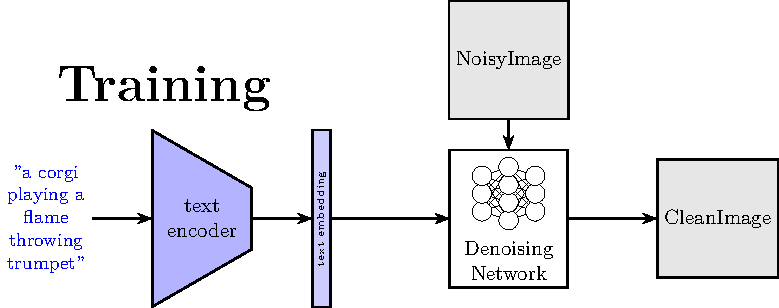
\includegraphics[width=\linewidth]{\toplevelprefix/chapters/chapter6/figs/tti-train.pdf}
    \caption{}
  \end{subfigure}
  \hfill
  \begin{subfigure}{0.47\textwidth}
    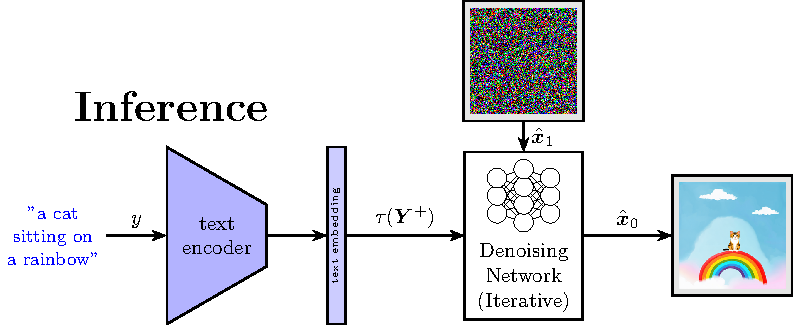
\includegraphics[width=\linewidth]{\toplevelprefix/chapters/chapter6/figs/tti-inf.pdf}
    \caption{}
  \end{subfigure}

  \caption{A high-level schematic of training and applying a text-to-image
  generative model, via conditional generation with a text prompt. \textbf{Left:}
  To train a text-to-image model, a large dataset of images paired with
  corresponding text captions is used. An encoder is used to map the captions to
  sequences of vectors, which are used as conditioning signals for a conditional
  denoiser, trained as described in \Cref{sub:cfg}. The text encoder may be
  pretrained and frozen, or jointly trained with the denoiser. \textbf{Right:}
  When applying a trained model, a desired text prompt is used as conditioning,
  then sampling is performed with the trained model, as in
  \Cref{alg:iterative_denoising_conditional_CFG} (\textit{mutatis mutandis} for
  use with an encoded text prompt). For full details of the process of encoding
  text to a sequence of vectors, see \Cref{sec:clm_text}.}
  \label{fig:text-to-image}
\end{figure}

Stable Diffusion follows the conditional generation methodology we outline in
\Cref{sub:cfg}, with two key modifications: (i) The conditioning signal is a
tokenized text prompt $\vY$, rather than a class label; (ii) Image denoising is
performed in ``latent'' space rather than on raw pixels, using a specialized,
pretrained variational autoencoder pair $f : \bR^{D_{\mathrm{img}}} \to
\bR^{d_{\mathrm{img}}}$, $g : \bR^{d_{\mathrm{img}}} \to
\bR^{D_{\mathrm{img}}}$ (see \Cref{sec:vae}), where $f$
is the encoder and $g$ is the decoder. Subsequent model development has shown that
point (ii) is an efficiency issue, rather than a core conceptual one, so we will
not focus on it, other than to mention that it simply leads to the following
straightforward modifications to the text-to-image pipeline sketched in
\Cref{fig:text-to-image}: 
\begin{enumerate}
  \item \textbf{At training time},
    the encoder $f : \vx \mapsto \vz$ is used to generate the denoising targets, and
    all denoising is performed on the encoded representations $\vz_t \in
    \bR^{d_{\mathrm{img}}}$;
  \item \textbf{At generation time}, sampling is performed on the
    representations $\hat{\vz}_t$, and
    the final image is generated by applying the decoder $g(\hat{\vz}_0)$.
\end{enumerate}
In contrast, issue (i) is essential, and the approach proposed to address it
represents one of the lasting methodological innovations of
\textcite{rombach2022high}.
In the context of the iterative conditional denoising framework we have
developed in \Cref{sub:cfg}, this concerns the parameterization of the denoisers
$\bar{\vz}_{\theta}(t, \vz_t, \vY^+)$.\footnote{In the setting of text
conditioning, the `augmented' label $\vY^+$, which is either the encoded text
prompt or $\varnothing$, denoting unconditional denoising, is often implemented
by mapping $\varnothing$ to the empty string ``'', then encoding this text
prompt with the tokenizer as usual. This gives a simple, unified way to treat
conditional and unconditional denoising with text conditioning.}
\textcite{rombach2022high} implement text conditioning in the denoiser using
a layer known as cross attention, inspired by the original encoder-decoder
transformer architecture of \textcite{vaswani2017attention}. Cross attention is
implemented as follows. We let $\tau : \bR^{D_{\mathrm{text}} \times N} \to
\bR^{d_{\mathrm{model}} \times N_{\mathrm{text}}}$
denote an encoding network for the text embeddings (often a causal
transformer---see \Cref{sec:clm_text}), and let $\psi : \bR^{d_{\mathrm{img}}}
\to \bR^{d_{\mathrm{model}} \times N_{\mathrm{img}}}$ denote the mapping corresponding to one of
the intermediate representations in the denoiser.\footnote{In practice,
text-conditioned denoisers add cross attention layers at regular intervals
within the forward pass of the denoiser, so $\psi$ should be seen as
layer-dependent, in contrast to $\tau$. See \textcite{rombach2022high} for
details.} Here, $N_{\mathrm{text}}$ is the maximum tokenized text prompt length,
and $N_{\mathrm{img}}$ roughly corresponds to the number of image channels
(layer-dependent) in the representation, which is fixed if the input image
resolution is fixed. Cross attention (with $K$ heads, and no bias) is defined as
    \begin{equation}
      \mathrm{MHCA}(\vz_t, \vY^+) \label{eq:mhca}
        = \vU_{\out}\mat{\SA([\vU_{\query}^{1}]^{\top}\psi(\vz_t),
        [\vU_{\attnkey}^{1}]^{\top}\tau(\vY^+), [\vU_{\val}^{1}]^{\top}\tau(\vY^+)) \\ \vdots \\
        \SA([\vU_{\query}^{K}]^{\top}\psi(\vz_t),
        [\vU_{\attnkey}^{K}]^{\top}\tau(\vY^+),
        [\vU_{\val}^{K}]^{\top}\tau(\vY^+))}, %
    \end{equation}
where $\mathrm{SA}$ denotes the ubiquitous self attention operation
in the transformer (which we recall in detail in \Cref{ch:applications}: see
\Cref{eq:mhsa,eq:self_attention}), and $\vU_{*}^{k} \in \bR^{d_{\mathrm{model}}\times
d_{\mathrm{attn}} }$ for $* \in \set{\mathrm{qry}, \mathrm{key}, \mathrm{val}}$
(as well as the output projection $\vU_{\mathrm{out}}$) are the learnable
parameters of the layer.

Notice that, by the definition of the self-attention operation, cross attention
\textit{outputs linear combinations of the value-projected text embeddings
weighted by correlations between the image features and the text embeddings.}
In the denoiser architecture used by \textcite{rombach2022high}, 
self-attention residual blocks in the denoiser architecture, applied to the
image representation at the current layer and defined analogously
to those in \Cref{eq:vit-res-block} for the vision transformer, are followed by cross
attention residual blocks of the form \eqref{eq:mhca}.
Such a structure requires the text encoder $\tau$ to, in a certain sense, share some
structure in its output with the image feature embedding $\psi$: this can be
enforced either by appropriate joint text-image pretraining (such as with CLIP
\cite{Radford2021-ir}) or by joint training with
the denoiser itself (which was proposed and demonstrated by
\textcite{rombach2022high}, but has fallen out of favor due to high data and
training costs for strong performance).
Conceptually, this joint text-image embedding space and the cross attention
layer itself bear a strong resemblance to the
conditional mixture of Gaussians denoiser that we derived in the previous
section (recall \eqref{eq:mog-conditional-denoising-unified-operator}), in the
special case of a single token sequence. Deeper
connections can be drawn in the multi-token setting following the rate reduction
framework for deriving deep network architectures discussed in
\Cref{ch:unrolling}, and manifested in the derivation of the CRATE
transformer-like architecture.

This same basic design has been further scaled to even larger model and dataset
sizes, in particular in modern instantiations of Stable Diffusion
\cite{DBLP:conf/icml/EsserKBEMSLLSBP24}, as well as in competing models such as
FLUX.1 \cite{Labs2025-fb}, Imagen \cite{Saharia2022-na}, and DALL-E \cite{Ramesh2022-nu}. 
The conditioning mechanism of cross attention has also become ubiquitous in
other applications, as in EgoAllo (\Cref{sub:ego-allo}) for conditioned pose generation and in Michelangelo \cite{zhao2023michelangelo} for conditional 3D shape generation based on images or texts. 






\section{Conditional Inference with Measurement Self-Consistency}
\label{sec:measurement-self-consistency}
In this last section, we consider the more extreme, but actually ubiquitous, case for distribution learning in which we only have a set of observed samples $\Y = \{\y_1,\ldots, \y_N\}$ of the data $\x$, but no samples of $\x$ directly! In general, the observation $\y \in \mathbb{R}^d$ is of lower dimension than $\x \in \mathbb{R}^D$. To make the problem well-defined, we do assume that the observation model between $\y$ and $\x$ is known to belong to a certain family of analytical models, denoted as $\y = h(\x, \theta) +\vw$, with $\theta$ either known or not known. 

Let us first try to understand the problem conceptually with the simple case when the measurement function $h$ is known and the observed $\y = h(\x) + \vw$ is informative about $\x$. That is, we assume that $h$ is surjective from the space of $\x$ to that of $\y$ and the support of the distribution $\y_0 = h(\x_0)$ is low-dimensional. This typically requires that the \textit{extrinsic} dimension $d$ of $\y$ is higher than the \textit{intrinsic} dimension of the support of the distribution of $\x$. Without loss of generality, we may assume that there exist functions:
\begin{equation}
F(\x) = \boldsymbol{0},\quad     G(\y) = \boldsymbol{0}.
\end{equation}
Notice that here we may assume that we know $G(\y)$ but not $F(\x)$. Let $\mathcal{S}_{\y} \doteq \{\y \mid G(\y) = \boldsymbol{0}\}$ be the support of $p(\y)$.  In general, $h^{-1}(\mathcal{S}_{\y}) = \{\x \mid G(h(\x)) = \boldsymbol{0}\}$ is a superset of $\mathcal{S}_{\x} \doteq \{\x \mid F(\x) = \boldsymbol{0}\}$. That is, we have $h(\mathcal{S}_{\x}) \subseteq \mathcal{S}_{\y}$.



\subsection{Linear Measurement Models}
First, for simplicity, let us consider that the measurement is a linear function of the data $\x$ of interest:
\begin{equation}
    \y = \vA\x.
\end{equation}
Here the matrix $\vA \in \mathbb{R}^{m\times n}$ is of full row rank and $m$ is typically smaller than $n$. We assume $\vA$ is known for now. We are interested in how to learn the distribution of $\x$ from such measurements. Since we no longer have direct samples of $\x$, we wonder whether we can still develop a denoiser for $\x$ with observations $\y$. Let us consider the following diffusion process:
\begin{equation}
    \y_t = \y_0 + t \vg, \quad \y_0 = \vA(\x_0), 
\end{equation}
where $\vg \sim \mathcal{N}(\boldsymbol{0}, \vI)$. 



Without loss of generality, we assume $\vA$ is of full row rank, i.e., under-determined. Let us define the corresponding process $\x_t$ as one that satisfies:
\begin{equation}
\y_t = \vA \x_t.   
\end{equation}

From the denoising process of $\y_t$, we have
\begin{equation}
    \y_{t-s} \approx  \y_t + st \nabla \log p_t(\y_t).
\end{equation}
Then we have:
\begin{equation}
    \vA\x_{t-s} \approx   \vA\x_t + st \nabla \log p_t(\vA \x_t),
\end{equation}
for a small $s >0$. So $\x_{t-s}$ and $\x_t$ need to satisfy:
\begin{equation}
    \vA(\x_{t-s} - \x_t) \approx st \nabla \log p_t(\vA\x_t). 
\end{equation}
Among all $\x_{t_s}$ that satisfy the above constraint, we arbitrarily choose the one that minimizes the distance $\|\x_{t-s} - \x_t\|_2^2$. Therefore, we obtain a ``denoising'' process for $\x_t$:
\begin{equation}
    \x_{t-s}  \approx \x_t + st\vA^\dagger \nabla \log p_t(\vA\x_t). 
\label{eqn:denoising-projection}
\end{equation}
Notice that this process does not sample from the distribution of $\vx_t$. In particular, there are components of $\vx$ in the null space/kernel of $\vA$ that can never be recovered from observations. Thus more information is needed to recover the full distribution of $\vx$, strictly speaking. But this recovers the component of $\vx$ that is orthogonal to the null space of $\vA$.





\subsection{3D Visual Model from Calibrated Images}
In practice, the measurement model is often nonlinear or only partially known. A typical problem of this kind is actually behind how we can learn a working model of the external world from the images perceived, say through our eyes, telescopes or microscopes. In particular, humans and animals are able to build a model of the 3D world (or 4D for a dynamical world) through a sequence of its 2D projections—a sequence of 2D images (or stereo image pairs). The mathematical or geometric model of the projection is generally known:
\begin{equation}
    \y^i = h(\x, \theta^i) +\vw^{i}, 
\end{equation}
where $h(\cdot)$ represents a (perspective) projection of the 3D (or 4D) scene from a certain camera view at time $t_i$ to a 2D image (or a stereo pair) and $\vw$ is some possibly additive small measurement noise. \Cref{fig:projection-2D} illustrates this relationship concretely, while \Cref{fig:inference_distributed} illustrates the model problem in the abstract. A full exposition of geometry related to multiple 2D views of a 3D scene is beyond the scope of this book. Interested readers may refer to the book \cite{MaY2003}. For now, all we need to proceed is that such projections are well understood and multiple images of a scene contain sufficient information about the scene.
\begin{figure}[t]
    \centering
    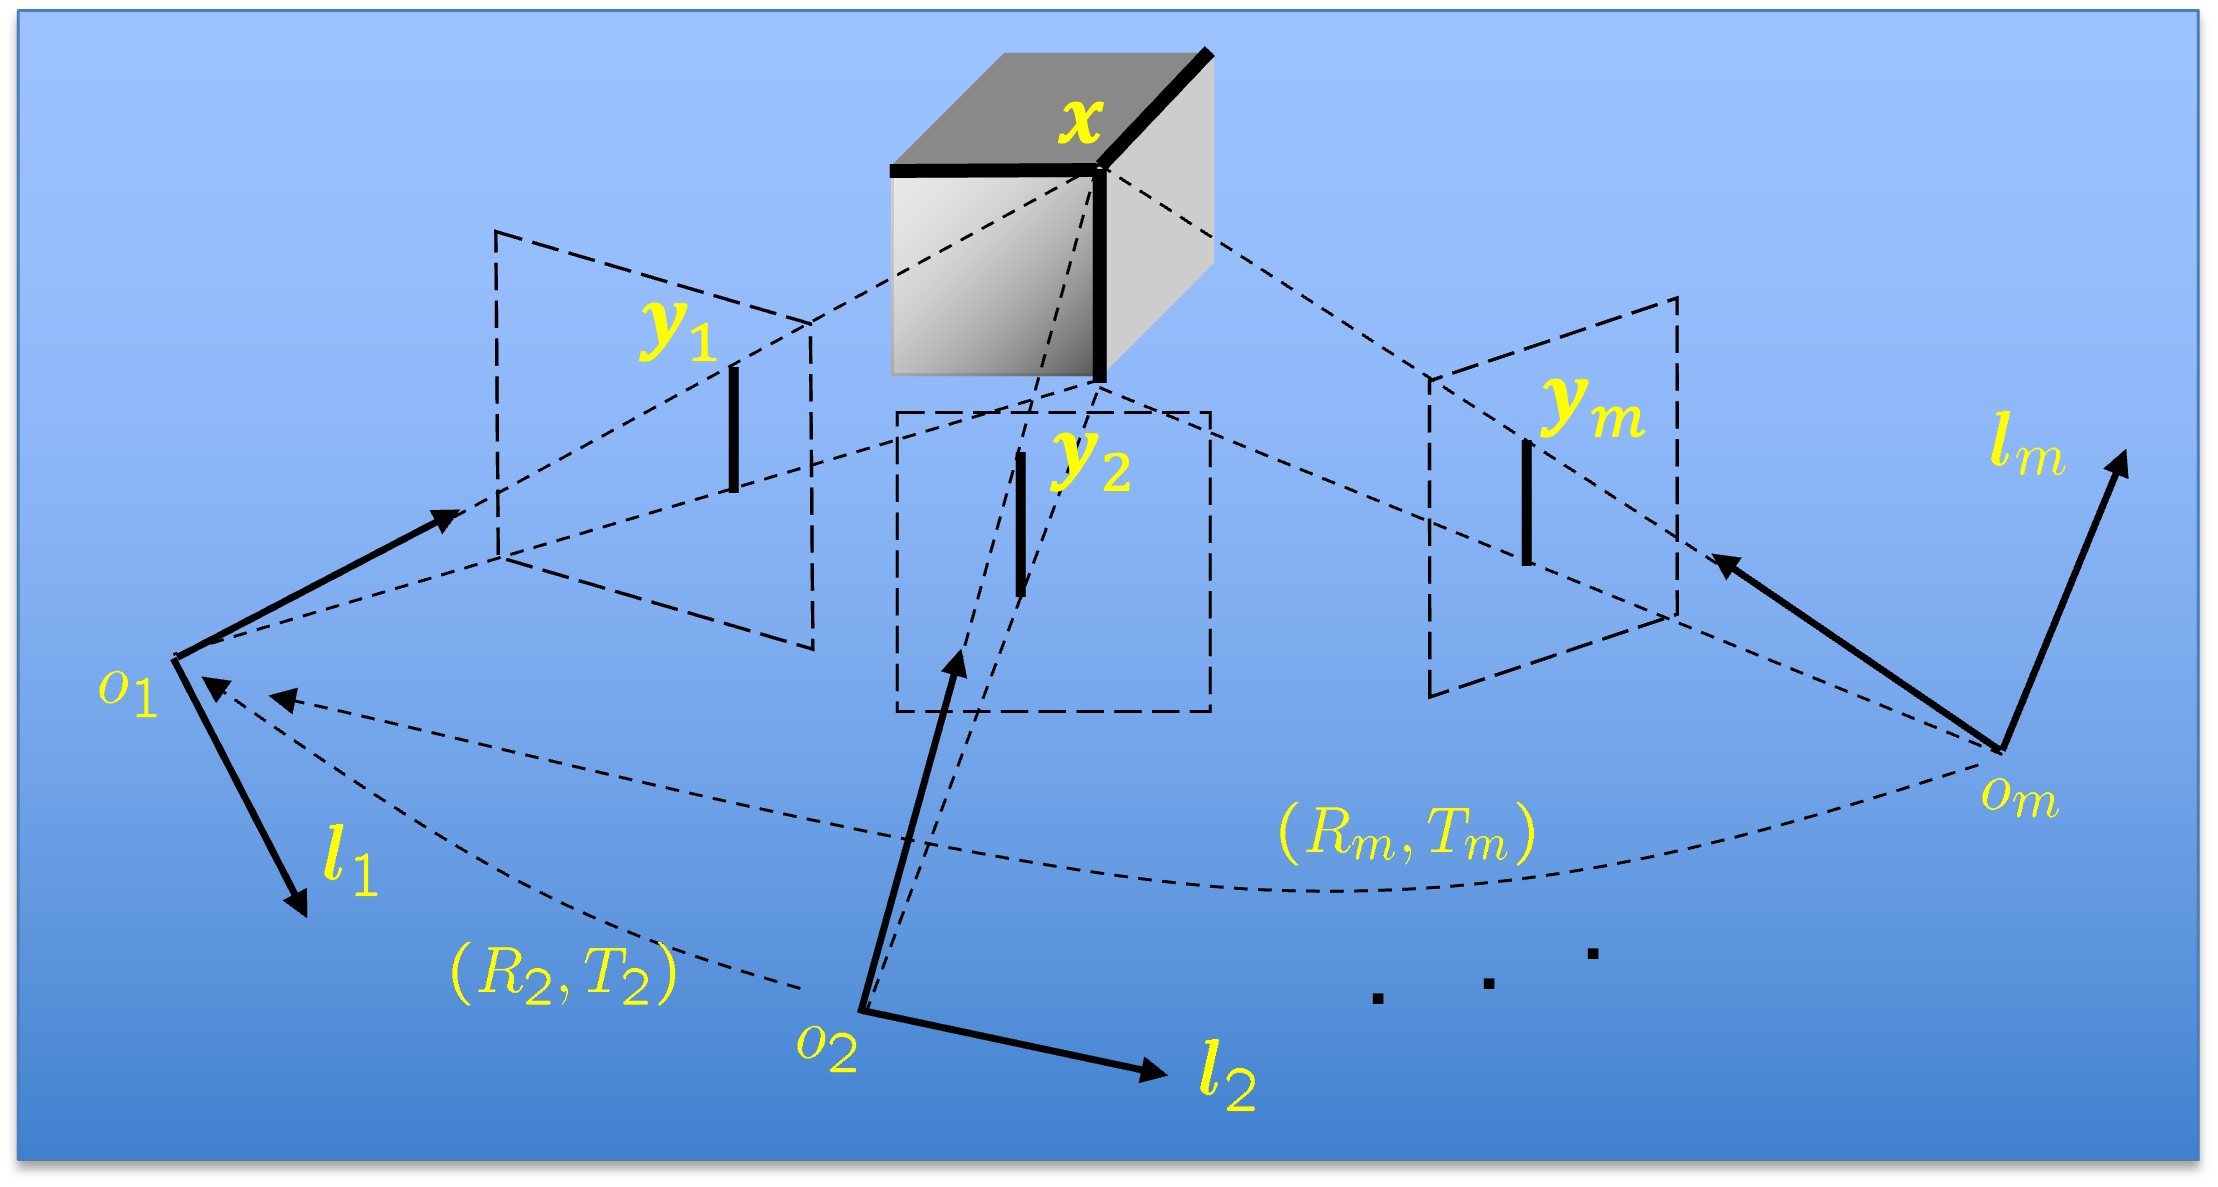
\includegraphics[width=0.7\linewidth]{\toplevelprefix/chapters/chapter6/figs/3D-2D-projection.png}
    \caption{Relationship between a 3D object/scene and its 2D projections. Here we illustrate the projection of a point $\x$ and a line intersecting the point.}
    \label{fig:projection-2D}
\end{figure}

\begin{figure}[t]
  \centering 
  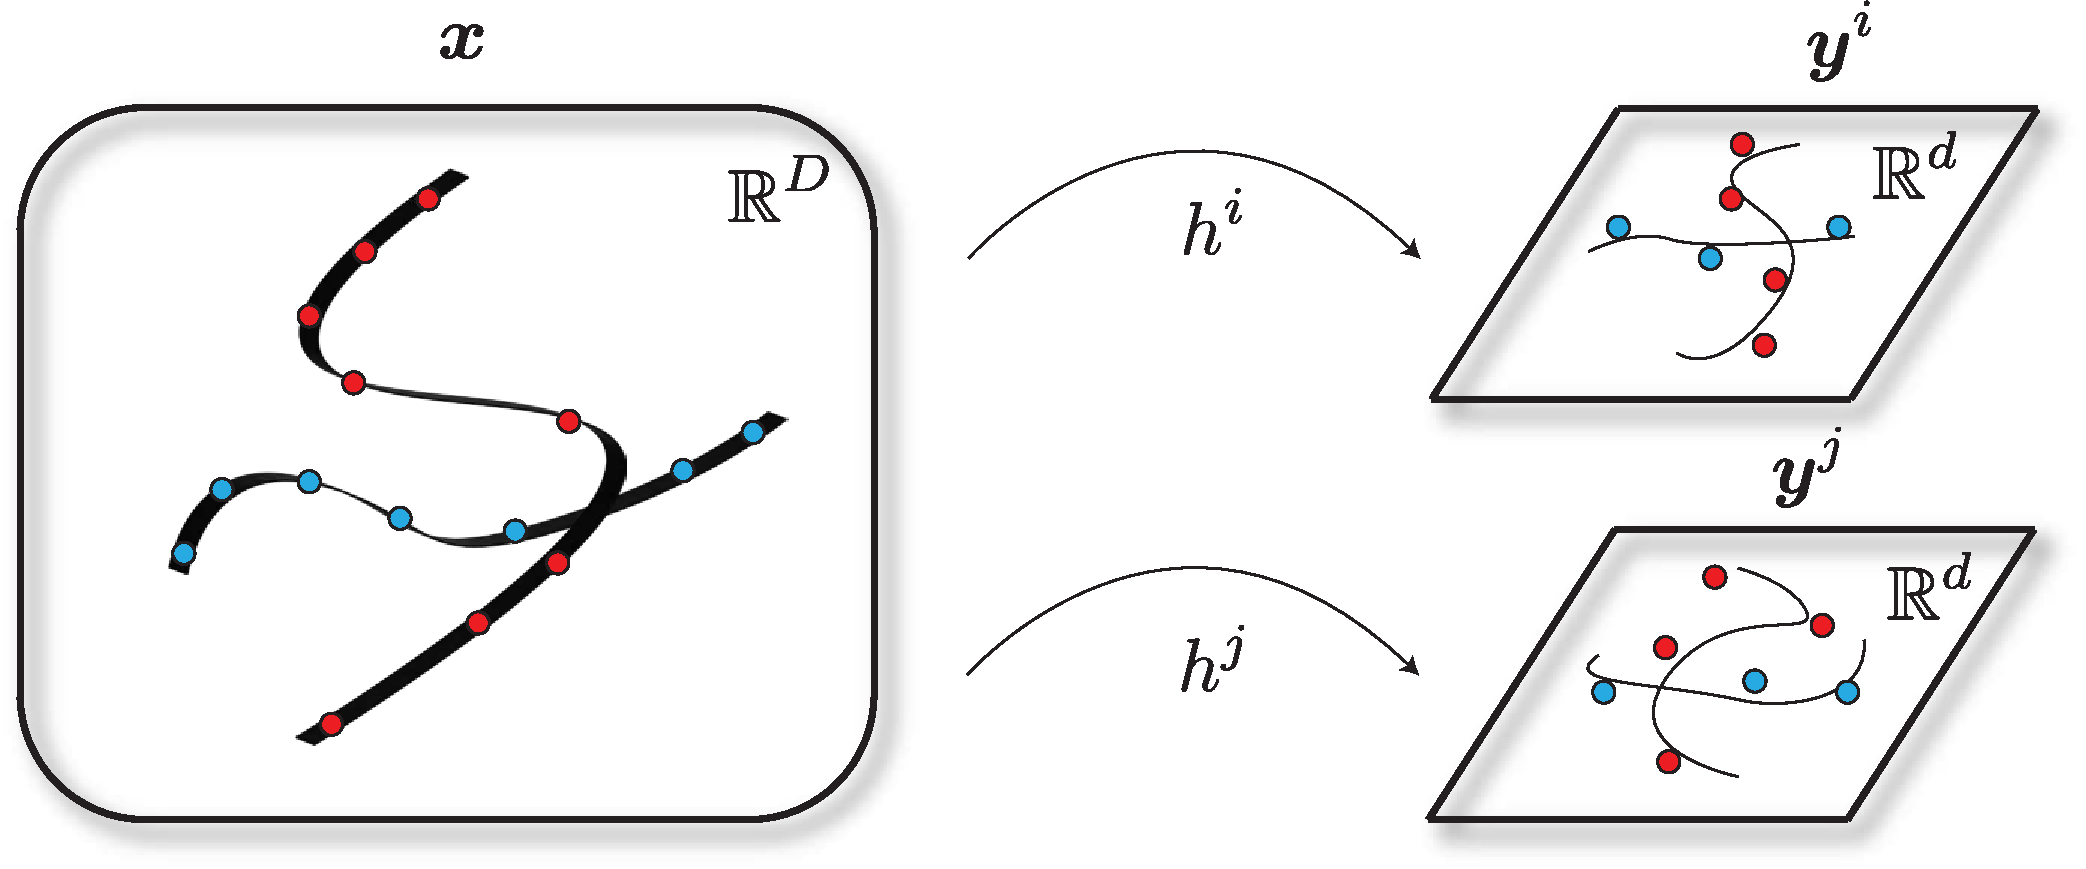
\includegraphics[width=0.7\linewidth]{\toplevelprefix/chapters/chapter6/figs/inference_distributed.pdf}
  \caption{\small \textbf{Inference with distributed measurements.} We have a low-dimensional distribution \(\vx\) (here, similarly to \Cref{fig:inference_roadmap}, depicted as a union of two \(2\)-dimensional manifolds in \(\R^{3}\)) and a measurement model \(\y^{i} = h^{i}(\vx) + \vw^{i}\). As before, we want to infer various properties of the conditional distribution of \(\vx\) given \(\vy\), where \(\vy\) is the collection of all the measurements \(\y^{i}\).}
  \label{fig:inference_distributed}
\end{figure}

In general, we would like to learn the distribution $p(\x)$ of the 3D (or 4D) world scene $\x$\footnote{Here by abuse of notation, we use $\x$ to represent either a point in 3D or a sample of an entire 3D object or a scene that consists of many points.} from the perceived 2D images of the world so far. The primary function of such a (visual) world model is to allow us to recognize places where we had been before or predict what the current scene would look like in a future time at a new viewpoint. 

Let us first examine the special but important case of stereo vision. In this case, we have two calibrated views of the 3D scene $\x$:
\begin{equation}
    \y^0 = h(\x, \theta^0) +\vw^0, \quad \y^1 = h(\x, \theta^1) +\vw^1, 
\end{equation}
where parameters $\theta_0$ and $\theta_1$ for the view poses can be assumed to be known. $\y^0$ and $\y^1$ are two 2D-projections of the 3D scene $\x$. We may also assume that they have the same marginal distribution $p(\y)$ and we have learned a diffusion and denoising model for it. That is, we know the denoiser:
\begin{equation}
  \bE[\vy \mid \vy_t=\vnu] =
  \vnu + t^2 \nabla_{\vnu}\log p_t(\vnu). 
 \label{eq:y-posterior-sampling-denoiser}    
\end{equation}
Or, furthermore, we may assume that we have a sufficient number of samples of stereo pairs $(\y^0, \y^1)$ and have also learned the joint distribution of the pairs. By a little abuse of notation, we also use $\y = h(\x)$ to indicate the pair $\y = (\y^0, \y^1)$ and $p(\y)$ as the learned probability distribution of the pair (say via a denoiser as above).  

The main question now is: How to learn (a representation for) the distribution of the 3D scene $\x$ from its two projections with known relationships? 
People might question the rationale for doing this: why is this necessary if the function $h(\cdot)$ is largely invertible? That is, the observation $\y$ can largely determine the unknown $\x$, which is kind of the case for stereo—in general, two (calibrated) images contain sufficient information about the scene depth, from the given vantage point. However, 2D images are far from the most compact representation of the 3D scene as the same scene can produce infinitely many (highly correlated) 2D images or image pairs. In fact, a good representation of a 3D scene should be invariant to the viewpoint. Hence, a correct representation of the distribution of 3D scenes should be much more compact and structured than the distribution of 2D images, stereo pairs, or image-depth pairs. 

Consider the (inverse) denoising process for the diffusion: $\y_t = \y + t\vg $ in \eqref{eq:y-posterior-sampling-denoiser}, where $\vg$ is standard Gaussian. From the denoising process of \eqref{eq:y-posterior-sampling-denoiser}, we have
\begin{equation}
    \y_{t-s} =  \y_t + st \nabla_{\y} \log p_t(\y_t).
\end{equation}
We try to find a corresponding ``denoising" process of $\x_t$ such that $\x$ is related to $y$ as:
\begin{equation}
    \y =  h(\x).
\end{equation}

Then we have:
\begin{equation}
    h(\x_{t-s}) \approx  h(\x_t) + st \nabla_{\y} \log p_t(h(\x_t)),
\end{equation}
for a small $s >0$. 
Suppose $\x_{t-s} = \x_t + s \vv$ for some vector $\vv$ and small increment $s$. We have
\begin{equation}
    h(\x_{t-s}) \approx h(\x_t) + \frac{\partial h}{\partial \x}(\vx_{t}) \cdot \vv s \doteq h(\x_t) + \vA(\x_t) \vv s. 
\end{equation}
Hence, we have
\begin{equation}
    \vA(\x_t) \vv = t \nabla_{\y} \log p_t(h(\x_t)).
    \label{eqn:pushforward}
\end{equation}
Geometrically the vector $\vv$ in the domain of $\x$ can be viewed as the pullback of the vector field $t \nabla \log p_t(\y)$ under the map $\y = h(\x)$. In general, as before, we may (arbitrarily) choose $\vv$ to be the minimum 2-norm vector that satisfies the pullback relationship. Hence, we can express  $\hat{\x}_{t-s}$ approximately as:
\begin{equation}
    \hat{\x}_{t-s} \approx \x_t + st\vA(\x_t)^\dagger \nabla_{\y} \log p_t(h(\x_t)). 
\label{eqn:pullback-denoise}
\end{equation}


\begin{remark}[Parallel Sensing and Distributed Denoising.]
{There is something very interesting about the above equation \eqref{eqn:pullback-denoise}. It seems to suggest we could try to learn the distribution of $\x$ through a process that is coupled with (many of) its (partial) observations:
\begin{equation}
\y^i = h^i(\x) +\vw^i, i =1, \ldots, K.
\end{equation} In this case, we obtain a set of equations that the vector field $\vv$ in the domain of $\x$ should satisfy:
\begin{equation}
    \vA^i(\x_t) \vv = t \nabla_{\y^i} \log p_t(h^i(\x_t)),
\label{eqn:federated-pushforward}
\end{equation}
where $\vA^i(\x_t) = \frac{\partial h^i}{\partial \x}(\vx_t)$. The final $\vv$ can be chosen as a ``centralized'' solution that satisfies all the above equations, or it could be chosen as a certain (stochastically) ``aggregated'' version of all $\vv^i$:
\begin{equation}
    \vv^i = t\vA^i(\x_t)^\dagger \big[\nabla_{\y^i} \log p_t(h^i(\x_t))\big], \quad i = 1, \ldots, K,
\end{equation}
that are computed in a parallel and distributed fashion? An open question here is exactly what the so-defined ``denoising'' process for $\x_t$ converges to, even in the linear measurement model case. When would it converge to a distribution that has the same low-dimensional support as the original $\x_0$, as $\y_t$ converges to $\y = h(\x_0)$? }
\end{remark}



\paragraph{Visual World Model from Uncalibrated Image Sequences}

In the above derivation, we have assumed that the measurement model $h(\cdot)$ is fully known. In the case of stereo vision, this is rather reasonable as the relative pose (and calibration) of the two camera views (or two eyes\footnote{The relative pose of our two eyes is well known to our brain.}) is usually known in advance. Hence, through the stereo image pairs, in principle we should be able to learn the distribution of 3D scenes, at least the ego-centric distribution of 3D scenes. However, the low-dimensional structures of the so-called learned distribution contain variation caused by changing the viewpoints. That is, the appearance of the stereo images varies when we change our viewpoints with respect to the same 3D scene. For many practical vision tasks (such as localization and navigation), it is important that we can decouple this variation of viewpoints from an invariant representation of (the distribution of) 3D scenes.

\begin{remark}Note that the above goal aligns well with Klein's Erlangen Program for modern geometry, which is to study invariants of a manifold under a group of transformations. Here, we may view the manifold of interest as the distribution of ego-centric representations of 3D scenes. We have learned that it admits a group of three-dimensional rigid-body motion acting on it. It is remarkable that our brain has learned to effectively decouple such transformations from the observed 3D world.
\end{remark}


Notice that we have studied learning representations that are invariant to translation and rotation in a limited setting in Chapter \ref{ch:representation}. We know that the associated compression operators take the necessary form of (multi-channel) convolutions, hence leading to the (deep) convolutional neural networks. Nevertheless, operators that are associated with compression or denoising that are invariant to more general transformation groups remain elusive to characterize \cite{cohen2016group}.  
For the 3D Vision problem in its most general setting, we know the change of our viewpoints can be well modeled as a rigid-body motion. However, the exact relative motion of our eyes between different viewpoints is usually not known. More generally, there could also be objects (e.g., cars, humans, hands) moving in the scene and we normally do not know their motion either. How can we generalize the problem of learning the distribution of 3D scenes with calibrated stereo pairs to such more general settings? More precisely, we want to learn a compact representation $\x$ of the 3D scenes that is invariant to the camera/eye motions. Once such a representation is learned, we could sample and generate a 3D scene and render images or stereo pairs from arbitrary poses. 


To this end, note that we can model a sequence of stereo pairs as:
\begin{equation}
    \y^k = h(\x^k, \theta^k), \quad k=1, \ldots, K,
\end{equation}
where $h(\cdot)$ represents the projection map from 3D to 2D. $\theta^k$ denotes the rigid-body motion parameters of the $k$th view, with respect to some canonical frame in the world. $\x^k$ represents the 3D scene at time $k$. If the scene is static, $\x^k$ should all be the same $\x^k = \x$. To simplify the notation, we may denote the set of $k$ equations as one:
\begin{equation}
    \Y = H(\x,\Theta). 
\end{equation}
We may assume that we are given many samples of such stereo image sequences $\{\Y_i\}$. The problem is how to recover the associated motion sequence $\{\Theta_i\}$ and learn the distribution of the scene $\x$ (that is invariant to the motion). To the best of our knowledge, this remains an open challenging problem, probably as the final frontier for the 3D Vision problem. 





\section{Summary and Notes}
\paragraph{Measurement matching without clean samples.} In our development of
conditional sampling, we considered measurement matching under an observation
model \eqref{eq:measurement-matching-observation}, where we assume that we have
paired data $(\vx, \vy)$—i.e., ground truth for each observation $\vy$.
In many practically relevant inverse problems, this is not the case: one of the
most fundamental examples is in the context of compressed sensing, which we
recalled in \Cref{ch:classic}, where we need to reconstruct $\vx$ from $\vy$
using prior knowledge about $\vx$ (i.e., sparsity).
In the setting of denoising-diffusion, we have access to an implicit prior for
$\vx$ via the learned denoisers $\bar{\vx}_{\theta}(t, \vxi)$. Can we still perform 
conditional sampling without access to ground truth samples $\vx$?

For intuition as to why this might be possible, we recall a classical example
from statistics known as Stein's unbiased risk estimator (SURE).
Under an observation model $\vx_t = \vx + t \vg$ with $\vg \sim \cN(\Zero,
\vI)$ and $t>0$, it turns out that for any weakly differentiable $f : \bR^D \to \bR^D$,
\begin{equation}\label{eq:sure-risk}
  \bE_{\vg}\left[
    \norm*{\vx - f(\vx + t \vg)}_2^2
    \right]
  =
  \bE_{\vg}\left[
    \norm*{\vx+t\vg - f(\vx + t \vg)}_2^2
    + 2t^2 \nabla \cdot f(\vx + t\vg)
    \right]
  - t^2 D,
\end{equation}
where $\nabla \cdot$ denotes the divergence operator:
\begin{equation*}
	\nabla \cdot f = \sum_{i=1}^D \partial_i f_i.
\end{equation*}
The $\vx$-dependent part of the RHS of \Cref{eq:sure-risk} is called Stein's unbiased risk
estimator (SURE). If we take expectations over $\vx$ in \Cref{eq:sure-risk},
note that the RHS can be written as an expectation with respect to $\vx_t$---in
particular, the mean-squared error of \textit{any denoiser $f$} can be estimated
\textit{solely from noisy samples}!
This remarkable fact, in refined forms, constitutes the basis for many practical
techniques for performing image restoration, denoising-diffusion, etc.\ using
only noisy data: notable examples include the ``noise2noise'' paradigm
\cite{pmlr-v80-lehtinen18a}
and Ambient Diffusion \cite{daras2023ambient}.

As a fun aside, we point out that \Cref{eq:sure-risk} leads to an alternate
proof of Tweedie's formula (\Cref{thm:tweedie}). At a high level, one takes
expectations over $\vx$ and expresses the main part of the RHS of
\Cref{eq:sure-risk} equivalently, via integration by parts, as
\begin{equation}
  \bE_{\vx_t}\left[
    \norm*{\vx_t - f(\vx_t)}_2^2
    + 2t^2 \nabla \cdot f(\vx_t)
    \right]
  =
  \bE_{\vx_t}\left[
    \norm*{\vx_t - f(\vx_t)}_2^2
    \right]
  - 2t^2 \int
  \ip*{\nabla p_{\vx_t}(\vxi)}{f(\vxi)}
  \odif \vxi.
\end{equation}
This is a quadratic function of $f$, and formally taking derivatives gives
that the optimal $f$ satisfies Tweedie's formula (\Cref{thm:tweedie}). This
argument can be made rigorous using basic ideas from the calculus of variations.


\paragraph{Corrections to the Diffusion Posterior Sampling (DPS) approximation.}
In \Cref{example:denoising-conditional-gaussian} and in particular in
\Cref{fig:conditional_sampling_computational_gaussian}, we pointed out
a limitation of the DPS approximation
\Cref{eq:conditional-posterior-measurementmatching-gaussian-case-dps-approx} at
small levels of measurement noise. 
This limitation is well-understood, and a principled approach to ameliorating it
has been proposed by Rozet et al.\ \cite{rozet2024learning}.
The approach involves incorporating an additional estimate for the variance of
the noisy posterior $p_{\vx \mid \vx_t}$ to
\Cref{eq:conditional-posterior-measurementmatching-gaussian-case-dps-approx}---we
refer to the paper for details.
Natural estimates for the posterior variance are slightly less scalable than DPS
itself due to the need to invert an affine transformation of the Jacobian of
the posterior denoiser $\bE[\vx \mid \vx_t=\vxi]$ (a large matrix). This is done
relatively efficiently by Rozet et al.\ \cite{rozet2024learning} using automatic differentiation and an
approximation for the inverse based on conjugate gradients. It seems that it
should be possible to improve further over this approach (say, using classical
ideas from second-order optimization).


\paragraph{More about measurement matching and diffusion models for inverse
problems.} 

Diffusion models have become an extremely popular tool for solving inverse
problems arising in scientific applications. Many more methods beyond the simple
DPS algorithm we have presented in \Cref{alg:iterative_denoising_conditional_DPS} have been
developed and continue to be developed, as the area is evolving rapidly.
Popular and performant classes of approaches beyond DPS, which we have presented
due to its generality, include variable splitting approaches like DAPS
\cite{Zhang2024-ha},
which allow for specific measurement constraints to be enforced much more
strongly than in DPS, and exact approaches that can avoid the use of
approximations as in DPS, such as TDS \cite{wu2023practical}.
For more on this area, we recommend \cite{zheng2025inversebench}, which
functions simultaneously as a survey and a benchmark of several popular methods
on specific scientific inverse problem datasets.

\section{Exercises and Extensions}


\begin{exercise}[Posterior Variance Correction to DPS]

  \begin{enumerate}
    \item Using the code provided in the book GitHub for implementing
      \Cref{fig:conditional_sampling_computational_gaussian}, implement the
      posterior variance correction proposed by \textcite{rozet2024learning}.
    \item Verify that it ameliorates the posterior collapse at low noise
      variance issue observed in
      \Cref{fig:conditional_sampling_computational_gaussian}.
    \item Discuss any issues of sampling correctness that are retained or
      introduced by the corrected method, as well as its efficiency, relative to
      diffusion posterior sampling (DPS).
  \end{enumerate}

\end{exercise}

\begin{exercise}[Conditional Sampling on MNIST]
  \begin{enumerate}
    \item Train a simple classifier for the MNIST dataset, using an architecture
      of your choice. Additionally train a denoiser suitable for use in
      conditional sampling (\Cref{alg:iterative_denoising_conditional_CFG},
      since this denoiser can be used for unconditional denoising as well).
    \item Integrate the classifier into a conditional sampler based on
      classifier guidance, as described in the first part of \Cref{sub:cfg}.
      Evaluate the resulting samples in terms of faithfulness to the
      conditioning class (visually; in terms of nearest neighbor; in terms of
      the output of the classifier).
    \item Integrate the classifier into a conditional sampler based on
      classifier-free guidance, as described in \Cref{sub:cfg} and
      \Cref{alg:iterative_denoising_conditional_CFG}. Perform the same
      evaluation as in the previous step, and compare the results.
    \item Repeat the experiment on the CIFAR-10 dataset.
  \end{enumerate}


\end{exercise}



\end{document}
